% !TeX root = ../main.tex

\chapter{高横动量希格斯玻色子衰变到双b夸克的标定}
\label{cha:Xbb}


%自从ATLAS实验和CMS实验在2012年发现希格斯玻色子~\cite{ATLASHIGGS,CMSHIGGS}之后,与之相关的一系列性质的精确测量变得非常重要,比如其自身性质、它与标准模型中其他粒子的耦合和它的产生模式和衰变,
%这些属性都能对标准模型进行严格验证。
%而这也是LHC上两个大型探测器ATLAS和CMS的主要任务之一,
ATLAS和CMS的其中一项重要任务就是对希格斯玻色子的性质进行精确的测量,
在2015年到2018年$Run\_2$计划期间,LHC将质心系能量提高到了13TeV,ATLAS探测器和CMS探测器在这期间收集到的可用于物理分析的数据总积分亮度分别为139$fb^{-1}$和137$fb^{-1}$,
并开展一系列与希格斯玻色子相关的研究,标准模型中希格斯玻色子的产生和衰变在第~\ref{sec:Higgs}~小节中有简要介绍,
这里在表~\ref{tab:ACHIGGS}~中总结了
%ATLAS实验和CMS实验进行的
与希格斯玻色子产生和衰变相关的一系列最新测量结果~\cite{ATLASHM,CMSHM},
ATLAS合作组和CMS合作组测得的组合希格斯玻色子信号强度
$\footnote{组合信号强度定义为测得的信号量与标准模型所预测的信号量的比值。}$分别为1.06$\pm$0.07和$1.02^{+0.07}_{-0.06}$,
并且由不同产生和衰变模式测得的信号强度都与标准模型的预期一致。

%ATLASHIGGS\cite{ATLASHIGGS1,ATLASHIGGS2,ATLASHIGGS3,ATLASHIGGS4,ATLASHIGGS5,ATLASHIGGS6,ATLASHIGGS7}
%CMSHIGGS\cite{CMSHIGGS1,CMSHIGGS2,CMSHIGGS3,CMSHIGGS4,CMSHIGGS5,CMSHIGGS6,CMSHIGGS7,CMSHIGGS8,CMSHIGGS9,CMSHIGGS10}
%ATLASHBB\cite{AHbb1,AHbb2,AHbb3,AHbb4,AHbb5,AHbb6,AHbb7,AHbb8,AHbb9}
%CMSHBB\cite{CHbb1,CHbb2,CHbb3,CHbb4}

\begin{table}[ht]
\caption{ATLAS实验和CMS实验进行的与希格斯玻色子产生和衰变相关的一系列最新测量结果。}
\begin{center}
\begin{adjustbox}{width=\columnwidth,center}
\begin{tabular}{c|cc|cc}
    \hline
    \hline
    \multirow{2}{*}{Analysis} & \multicolumn{2}{c|}{ATLAS} & \multicolumn{2}{c}{CMS} \\
    & Production tags & \thead{Luminosity($fb^{-1}$) \\ and References} & Production tags & \thead{Luminosity($fb^{-1}$) \\ and References} \\
    \hline
    $H\rightarrow\gamma\gamma$ & \thead{ggF,VBF,WH\\ZH,$t\bar{t}H$,tH} & 139\cite{ATLASHIGGS1} & ggF,VBF,$t\bar{t}$H & 35.9\cite{CMSHIGGS2},41.5\cite{CMSHIGGS3},77.4\cite{CMSHIGGS1} \\
    \hline
    $H\rightarrow ZZ^*$ & \thead{ggF,VBF,WH\\ZH,$t\bar{t}H$,tH} & 36.1\cite{ATLASHIGGS5,AHbb10},139\cite{ATLASHIGGS2} & \thead{ggF,VBF,VH\\$t\bar{t}H$}& 137\cite{CMSHIGGS4}  \\
     \hline
    $H\rightarrow WW^*$ & ggF,VBF,$t\bar{t}H$ & 36.1\cite{ATLASHIGGS3,ATLASHIGGS5,AHbb10} & \thead{ggF,VBF,VH\\WH,ZH} & 35.9\cite{CMSHIGGS5}  \\
     \hline
    $H\rightarrow \tau\tau$ & ggF,VBF,$t\bar{t}H$ & 36.1\cite{ATLASHIGGS4,ATLASHIGGS5,AHbb10} & ggF,VBF,VH & 35.9\cite{CMSHIGGS6},77.4\cite{CMSHIGGS7}   \\
     \hline
    $H\rightarrow b\bar{b}$ & \thead{VBF,WH,ZH\\$t\bar{t}H$}  & 30.6\cite{AHbb6},36.1\cite{AHbb7,AHbb8},139\cite{AHbb5} & \thead{ggF,WH,ZH\\$t\bar{t}H$} & 35.9\cite{CHbb3},41.5\cite{CHbb2,CHbb4},77.4\cite{CHbb1} \\
     \hline
    $H\rightarrow \mu\mu$ & \thead{ggF,VBF,VH\\$t\bar{t}H$} & 139\cite{ATLASHIGGS6} & ggF,VBF& 35.9\cite{CMSHIGGS10}  \\
    \hline
    \hline
\end{tabular}
\end{adjustbox}
\end{center}
\label{tab:ACHIGGS}
\end{table}

其中$H\rightarrow b\bar{b}$衰变道是希格斯玻色子的主要衰变模式,
在探测器中,来自高横动量希格斯玻色子衰变的两个b-jet接近准直,
会合并到一个LR-jet当中,但是来自QCD过程和t夸克衰变的本底非常大。
对高横动量$H\rightarrow b\bar{b}$衰变的精确标定可以显著提升
ggF
%、VBF
和tH产生模式中$H\rightarrow b\bar{b}$衰变的测量精度,
并有望能填补ATLAS合作组在这一块测量的空缺,
而且
%在
许多超出标准模型的新物理
%模型中
~\cite{BSMHIGGS1,BSMHIGGS2,BSMHIGGS3}
也预言了能与标准模型中希格斯玻色子耦合的新粒子的存在,
%都引入了能与标准模型中希格斯玻色子耦合的新粒子的存在,
对高横动量$H\rightarrow b\bar{b}$衰变的精确标定对新物理的寻找也有着重要意义。
%因此对高横动量的$H\rightarrow b\bar{b}$衰变的研究或者标定对希格斯玻色子性质的精确测量和新物理的寻找都有着重要意义。

%其中,尽管$H\rightarrow b\bar{b}$衰变道是希格斯玻色子的主要衰变模式,占高达$58\%$的分支比,
%但是也因为来自QCD过程和t夸克衰变的本底非常大,使得在LHC上面观测这个衰变模式变得很困难。
%通过要求事例中包含孤立的轻子,可以显著的降低QCD本底,因此寻找$H\rightarrow b\bar{b}$衰变道灵敏度最高的产生模式是VH,
%ATLAS合作组和CMS合作组在2018年分别利用$79.8fb^{-1}$和$41.3fb^{-1}$的数据通过VH产生模式观测到显著的$H\rightarrow b\bar{b}$事例,
%显著性分别达到了4.9和4.8倍的标准差~\cite{AHbb8,CHbb3},
%随后在2020年,ATLAS合作组利用$139fb^{-1}$的数据观测到了更加丰富的事例~\cite{AHbb5}。
%但是也有一部分研究在其他产生模式下测量$H\rightarrow b\bar{b}$的衰变,比如$t\bar{t}H$~\cite{AHbb7,AHbb8,CHbb1}、VBF~\cite{AHbb6}和高横动量区的ggF~\cite{CHbb3}。

%而高横动量的$H\rightarrow b\bar{b}$衰变与低横动量的$H\rightarrow b\bar{b}$衰变拓扑性质不一样,
%如图~\ref{fig:Boosted}~所示,在探测器中,来自高横动量希格斯玻色子衰变的两个b夸克接近准直,
%会合并到一个LR-jet当中,依靠其整体性使得$H\rightarrow b\bar{b}$事例更容易鉴定。
%而且在许多超出标准模型的新物理模型中~\cite{BSMHIGGS1,BSMHIGGS2,BSMHIGGS3}都引入了能与标准模型中希格斯玻色子耦合的新粒子的存在,
%这些新粒子的质量都很大,衰变产生的希格斯玻色子将会具有很高的横动量。
%因此对高横动量的$H\rightarrow b\bar{b}$衰变的研究或者标定对希格斯玻色子性质的精确测量和新物理的寻找都有着重要意义。

%\begin{figure}
  %\begin{center}
  %  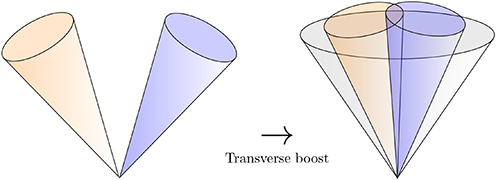
\includegraphics[width=0.75\textwidth]{figuresXbb/Boosted.jpg}
  %\end{center}
  %\caption{
%来自高横动量希格斯玻色子衰变的两个b夸克接近准直,从而合并到一个LR-jet当中。
  %}
    %\label{fig:Boosted}
%\end{figure}



\section{研究背景}
\label{sec:XbbBKG}


%TAGGING~\cite{TAGGING1,TAGGING2,TAGGING3,TAGGING4}
ATLAS合作组
%早在2014年
很早
就开始研究强子型衰变的LR-jet标定算法。
包括高横动量的希格斯玻色子的标定,
最早在2014年,
合作组利用LR-jet中subjet的味标定信息对LR-jet进行标定,
并使用了基于内部探测器中径迹的subjet重建算法,
同时优化了距离参数R~\cite{TAGGING1},
与第~\ref{sec:JET}~小节介绍的基于量能器拓扑集群的重建算法相比,
由于b-jet标定算法仅使用径迹的信息,
基于径迹的subjet可以针对b-jet标定性能进行独立的优化和校准,
并通过“幻影”关联与基于拓扑集群的jet匹配。
%将在第~\ref{sec:XbbORSR}~小节中介绍。
%在b强子识别方面将更加有效;
%它是利用LR-jet中subjet基于提升决策树的高级算法实现对LR-jet的标定的,并优化了距离参数R~\cite{TAGGING1},
随后在$Run\_2$计划期间合作组沿用了这一标定方法并开始使用优化后的距离参数R~\cite{TAGGING5},
并且后续为了更好的提高高横动量希格斯玻色子标定的性能,合作组
进一步优化了基于径迹的subjet重建算法~\cite{ATL-PHYS-PUB-2017-010},
将在第~\ref{sec:XbbORSR}~小节中介绍。
%还发展了专用的subjet重建算法~\cite{ATL-PHYS-PUB-2017-010}。

而在2015年左右
高横动量
%强子化
的W玻色子~\cite{TAGGING3}和t夸克的标定~\cite{TAGGING2}中,
它们利用
%了
LR-jet
的整体和内部性质发展了一系列低级算法和相应的变量(Jet substructure, JSS)用于LR-jet的标定,
称为LR-jet的结构变量,
表~\ref{tab:JSS}~总结了这些标定技术和相应的变量,
第~\ref{sec:XbbORJSS}~小节将对
其中一部分
%它们
做简要介绍。
后来合作组利用神经网络和提升决策树将这些结构变量整合到更高级的LR-jet标定算法当中~\cite{ATL-PHYS-PUB-2017-004},
这个算法的性能有了显著的提升,
%使得标定效率有了显著提升,
但是
%随之而来
也引入了一个困难,
如图~\ref{fig:MSCULP}~所示,
其中绿色实线表示QCD样本中LR-jet的质量分布,
而深红色虚线表示被基于神经网络的高级算法标定之后的LR-jet质量分布,
%蓝色虚线表示被基于提升决策树的高级算法标定之后的LR-jet质量分布。
可以看到基于神经网络
%和提升决策树
的高级算法学会了利用LR-jet质量来%信息
区分信号和本底,
%也就是
在被高级算法标定后,QCD样本中的LR-jet的质量分布会失真,
%并
变成了类似于W玻色子的质量分布的形状,
%使得
这种高级算法与LR-jet的质量表现出非常大的非线性相关性,
这在%实际的
利用质量谱测定散射截面或寻找新物理的分析中是不允许出现的。

\begin{table}[ht]
\caption{用于高横动量W玻色子和t夸克标定的各种低级算法和对应的变量。称为LR-jet的结构变量。}
\begin{center}
\begin{adjustbox}{width=\columnwidth,center}
\begin{tabular}{c|c|c}
    \hline
    \hline
    Observable & Variable & Tagging and reference \\
    \hline  
    Energy correlation ratios & \thead{$ECF_1,ECF_2$\\$ECF_1,C_2,D_2,e_3$} & t,W\cite{JSS1,JSS2} \\
    \hline  
    N-subjettiness & \thead{$\tau_1,\tau_2,\tau_3$\\$\tau_{21},\tau_{32}$} & t,W\cite{JSS3,JSS4} \\
    \hline  
    Center of mass observables & \thead{Fox Wolfram($R_2^{FW}$)\\Sphericity(S)\\Thrust($T_{MIN},T_{MAJ}$)} & W\cite{JSS5,JSS6,JSS7}  \\
    \hline  
    Splitting Measures & \thead{$Z_{CUT12},\mu_{12}$\\$\sqrt{d_{12}},\sqrt{d_{23}}$} & \thead{W\cite{JSS8,JSS9}\\t,w\cite{JSS10}} \\
    \hline  
    Planar Flow & $\mathcal{P}$& W\cite{JSS11} \\
    \hline  
    Dipolarity & $\mathcal{D}$ & W\cite{JSS12} \\
    \hline  
    Angularity & $a_3$ & W\cite{JSS13} \\
    \hline  
    Aplanarity & $A$ & W\cite{JSS6} \\
    \hline  
    KtDR & $KtDR$ & W\cite{JSS14} \\
    \hline  
    Qw & $Q_w$ & W\cite{JSS8} \\
    \hline
    \hline
\end{tabular}
\end{adjustbox}
\end{center}
\label{tab:JSS}
\end{table}


%后来合作组利用神经网络和提升决策树将这些变量整合到更高级的LR-jet标定算法当中~\cite{ATL-PHYS-PUB-2017-004},
%使得标定效率有了显著提升,但是随之而来也引入了一个困难,
%如图~\ref{fig:MSCULP}~所示,
%其中绿色实线表示QCD样本中LR-jet的质量分布,
%而深红色虚线表示被基于神经网络的高级算法标定之后的LR-jet质量分布,
%蓝色虚线表示被基于提升决策树的高级算法标定之后的LR-jet质量分布。
%可以看到基于神经网络和提升决策树的高级算法学会了利用LR-jet质量信息区分信号和本底,
%也就是在被高级算法标定后,QCD样本中的LR-jet的质量分布会失真,并变成类似于W玻色子的质量分布,
%使得这种高级算法与LR-jet的质量表现出非常大的非线性相关性,
%这在实际的利用质量谱测定散射截面或寻找新物理的分析中是不允许出现的。

\begin{figure}
  \begin{center}
    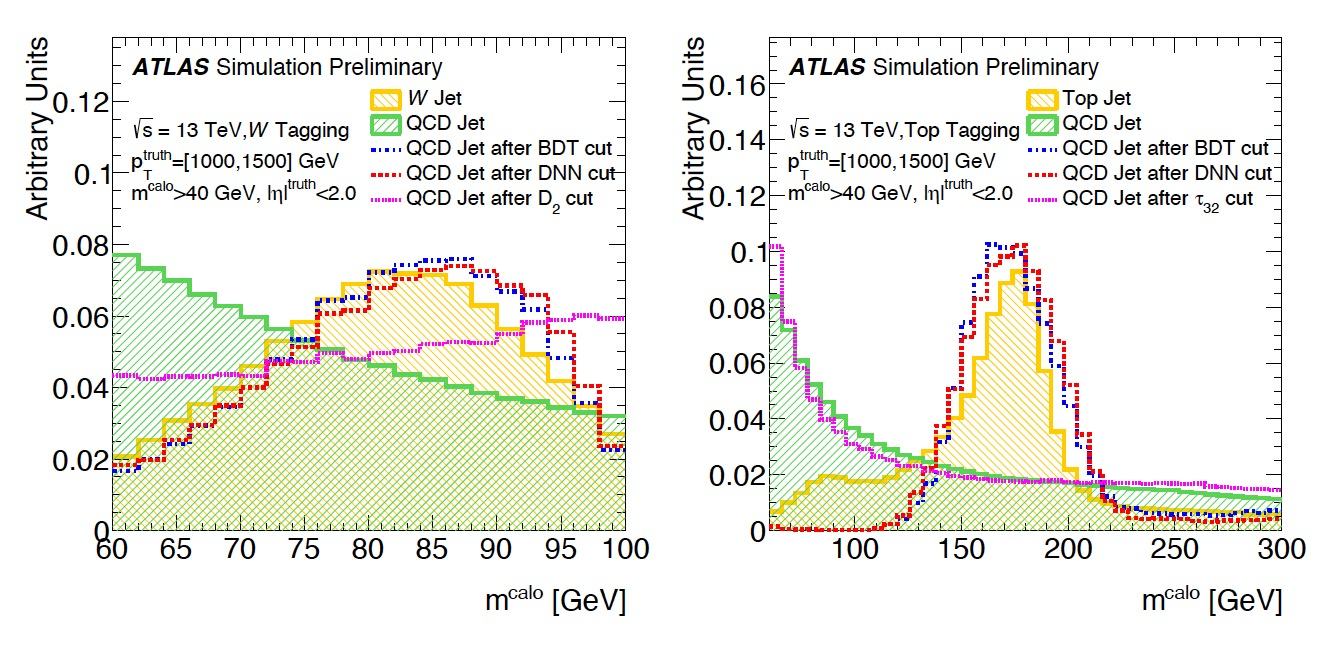
\includegraphics[width=0.9\textwidth]{figuresXbb/MSCULP.jpg}
  \end{center}
  \caption{
在被
%基于神经网络(DNN)和提升决策树(BDT)的
高级算法标定前和标定后,信号和本底中LR-jet的质量分布。
左图是W玻色子标定,右图为t夸克标定。
  }
    \label{fig:MSCULP}
\end{figure}



针对这一问题,合作组在2018年提出了多种去质量关联的技术~\cite{ATL-PHYS-PUB-2018-014}:
专用去相关标定算法(Designed decorrelated taggers, DDT)~\cite{DDT}、
k近邻回归方法(Fixed-efficiency k-nearest neighbours regression, k-NN)~\cite{KNN}和
卷积结构方法(Convolved substructure, CSS)~\cite{CSS}
提供了三种解除JSS与LR-jet质量之间关联性的解析方法;
而对抗性神经网络(Adversarial neural networks, ANN)~\cite{ANN}和
自适应增强方法(Adaptive boosting for uniform efficiency, uBoost)~\cite{UBOOST}则是
通过降低
%基于机器学习的
高级算法与LR-jet质量之间的相关性来解决这个问题。
其中基于对抗性神经网络的算法能比较成功的实现去质量关联性,
但是区分精度却明显的降低了,
%但是是以牺牲精确度为代价,
图~\ref{fig:ANNROC}~展示
%的是
了对于上述几种去质量关联的算法,
在高横动量的W玻色子标定中,
%来自W玻色子的
信号
%jet
标定效率\footnote{效率定义为算法标定的物理对象数目与用到的物理对象总数的比值。}
与
%来自QCD过程的
本底排除率\footnote{排除率定义为用到的物理对象总数与算法标定的物理对象数目的比值。}
的变化关系~\cite{ATL-PHYS-PUB-2018-014},
左图为低横动量区间[200,500]GeV,右图为横高动量区间[500,1000]GeV,
不同颜色的虚线对应不同的去质量关联算法,
在信号效率相等的情况下,本底排除率越高说明算法的性能越好,
可以看到,
$Z_{ANN}$相对于$Z_{NN}$来说,存在一定程度的性能损失,
其中$Z_{ANN}$是基于对抗性神经网络的去质量关联算法,
而$Z_{NN}$是基于神经网络,与LR-jet的质量有非常大的相关性。
%基于对抗性神经网络的去质量关联算法$Z_{ANN}$相对于基于神经网络的表现出质量相关性的算法$Z_{NN}$来说,
%存在一定程度的性能损失。


\begin{figure}
  \begin{center}
    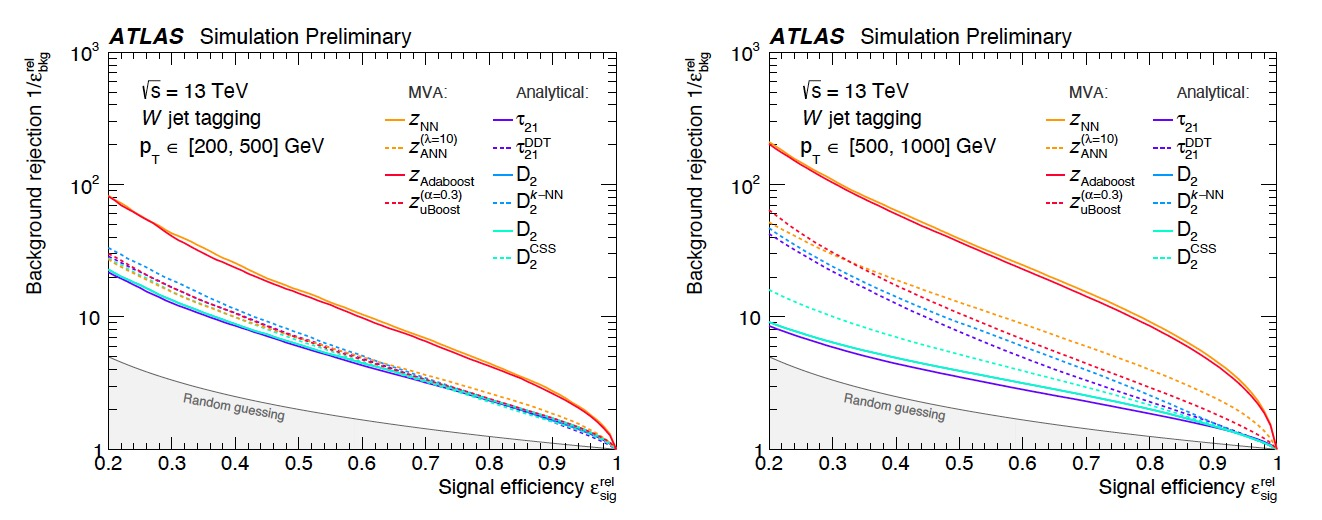
\includegraphics[width=0.9\textwidth]{figuresXbb/ANN.jpg}
  \end{center}
  \caption{对于不同的去质量关联算法,%~\cite{ATL-PHYS-PUB-2018-014},
在高横动量的W玻色子标定中,
  %来自W玻色子的
  信号标定效率与本底排除率的变化关系。
其中$Z_{ANN}$是基于对抗性神经网络的去质量关联算法,
而$Z_{NN}$是基于神经网络,与LR-jet的质量有非常大的相关性。
%其中LR-jet质量满足m$\in$[600,1000]GeV,
左图为低横动量区间[200,500]GeV,右图为横高动量区间[500,1000]GeV。
}
    \label{fig:ANNROC}
\end{figure}


同时,在高横动量希格斯玻色子的标定方面,
合作组希望结合之前沿用的技术
%即基于LR-jet中subjet的标定算法和
%高横动量的
和高横动量W玻色子、t夸克的标定技术,
发展一种
%基于神经网络的
既能实现去质量关联又能保持
%高精确度
高区分精度
的高级算法。
但在经过两轮研究人员的尝试之后,
发现始终不能同时保证去质量关联和高区分精度,
我在2019年初接手这个任务之后,在尝试原有方法不可行的同时,
也开始尝试新方法,
最后成功同时解决了这个问题。
%发展出一种既能实现去质量关联又能保持高精确度的高级算法。

本章将会展示,
%的是,
基于前馈型深度学习神经网络~\cite{FDNN}和变量控制的方法,利用LR-jet的运动学变量和其中subjet的
味标定信息,
%高级标定算法,
实现一种既能实现去质量关联又能保持高区分精确的高横动量$H\rightarrow b\bar{b}$标定算法。
其中第~\ref{sec:XbbSimS}~小节将会介绍新算法开发所用到的MC样本,
包括高横动量$H\rightarrow b\bar{b}$信号和来自t夸克和QCD过程的两种主要本底;
第~\ref{sec:XbbOR}~小节将会介绍事例的重建和筛选技术,
也包括LR-jet与subjet的匹配、所使用的b-jet标定算法和LR-jet结构变量等;
第~\ref{sec:XbbTagger}~小节则会详细介绍新算法的设计思路,包括输入变量控制、加权策略分析和结构参数优化等;
第~\ref{sec:XbbPerf}~小节将介绍新算法的性能及其与ATLAS合作组最新算法的对比,
包括质量关联性、区分因子和本底排除率随信号效率的变化关系对比等;
第~\ref{sec:XbbCon}~小节是章节总结。


\section{MC样本}
\label{sec:XbbSim}

\subsection{信号}
\label{sec:XbbSimS}

为了产生丰富的信号事例,
高横动量的$H\rightarrow b\bar{b}$%事例的希格斯玻色子
是由MC模拟的
%超出标准模型的
Randall-Sundrum额外维模型~\cite{Randall:1999ee}产生。
模型中的
%Kaluza-Klein
KK引力子能与标准模型中希格斯玻色子耦合,%其中耦合参数被设置为$k/\bar{M}_P=1$,
并衰变成两个希格斯玻色子,希格斯玻色子的质量设置为125GeV,
两个希格斯玻色子随后均衰变为$b\bar{b}$夸克对。
其中耦合参数被设置为$k/\overline{M}_P=1$,k是曲率参数(The curvature parameter),
$\overline{M}_P$是普兰克质量刻度(The Planck mass scale)。

%事例是使用领头阶NNPDF2.3部分子分布函数~\cite{Martin:2009iq}和\textsc{ATLAS A14}校准参数集~\cite{ATL-PHYS-PUB-2014-021}
%并通过\textsc{Pythia 8.186}~\cite{Sjostrand:2007gs}和\textsc{MadGraph5}~\cite{Alwall:2014hca}模拟产生。
事例是由\textsc{Pythia 8.186}~\cite{Sjostrand:2007gs}和\textsc{MadGraph5}~\cite{Alwall:2014hca}模拟产生,
模拟过程中使用领头阶NNPDF2.3部分子分布函数~\cite{Martin:2009iq}和\textsc{ATLAS A14}潜在事例校准参数集~\cite{ATL-PHYS-PUB-2014-021}。
当KK引力子和希格斯玻色子之间的质量差距足够大,
%的情况下
%可以迫使
可使得衰变出来的希格斯玻色子具有高横动量,
因此,这里模拟的KK引力子质量有:300、400、500、600、700、800、900、1000、1100、1200、1300、1400、1500
、1600、1800、2000、2250、2500、2750、3000、3500、4000、4500、5000、6000GeV。
信号样本以合适的比例覆盖了感兴趣的高横动量区域,
并且,模拟过程中要求希格斯玻色子只衰变到$b\bar{b}$夸克对。
%可以使信号样本以合适的比例覆盖感兴趣的高横动量区域,这些MC样本中,希格斯玻色子只衰变到$b\bar{b}$夸克对。
%各个引力子质量不同的样本最后会合并在一起并且重新赋予权重,使得其中LR-jet的横动量分布和QCD样本中的一致,
为了减小样本之间的运动学差异带来的影响,
所有样本最后会合并在一起重新加权,
使得事例中横动量最高即领头LR-jet的横动量分布与QCD
%样本
本底
中的分布一致,
用于后续算法性能的评估和对比。
接下来将会介绍QCD
%样本
本底的模拟和产生。
%加权是为了减小由未加权的样本之间的运动学差异带来的影响。
%下一小节也就是第小节将会介绍其中一种本底高横动量的QCD过程的模拟。
%这样加权是为了减小由未加权的样本之间的运动学差异带来的影响。


\subsection{本底}
\label{sec:XbbSimB}

这里考虑了两种本底:一种是来自QCD过程
的高能轻夸克或胶子辐射,
%高横动量的夸克胶子相互作用或胶子自相互作用,
记为multijet,
%模拟的multijet
样本中事例的领头LR-jet
%也就是横动量最高的LR-jet
的横动量分布如图~\ref{fig:bkg-pt}~所示,这也是真实数据中的分布形状,
%具有这种物理分布
这种分布的样本之后会用于第~\ref{sec:XbbTagger}~小节和第~\ref{sec:XbbPerf}~小节中新算法性能的评估和对比;
%具有这种物理分布的样本会用于第~\ref{sec:XbbTagger}~小节和第~\ref{sec:XbbPerf}~小节中算法性能的评估和对比;
另一种来自于%强子型衰变的
高横动量的t夸克衰变,
t夸克主要的衰变模式~\cite{PDG}是$t\to b W^{+}$、$\bar{t}\to \bar{b} W^{-}$。
%的LR-jet,
%同样
为了产生丰富的t夸克,
%事例,
%t夸克
样本是
%由$Z\prime$模型中
由高质量$Z' \to t\bar{t}$衰变产生~\cite{ZTT},
%所
模拟的$Z\prime$质量有:
400、500、750、1000、1250、1500、1750、2000、2250、2500、2750、3000、4000、5000GeV。
同样,所有样本最后会合并在一起并重新加权,
使事例中领头LR-jet的横动量分布与QCD
%样本
本底
中的分布一致。
%使得最后LR-jet的横动量分布和QCD样本中的一致,
模拟过程中要求t夸克以强子型末态模式衰变,
即衰变产生的W玻色子会衰变成两个夸克。
%而且这些MC样本中,t夸克只允许强子型衰变。
这两种本底
%样本
都是由\textsc{Pythia 8.186}模拟产生,
使用领头阶NNPDF2.3部分子分布函数和\textsc{ATLAS A14}校准参数集。
%都是使用领头阶NNPDF2.3部分子分布函数和\textsc{ATLAS A14}校准参数集
%并通过\textsc{Pythia 8.186}~\cite{Sjostrand:2007gs}模拟产生的。

\begin{figure}
  \begin{center}
    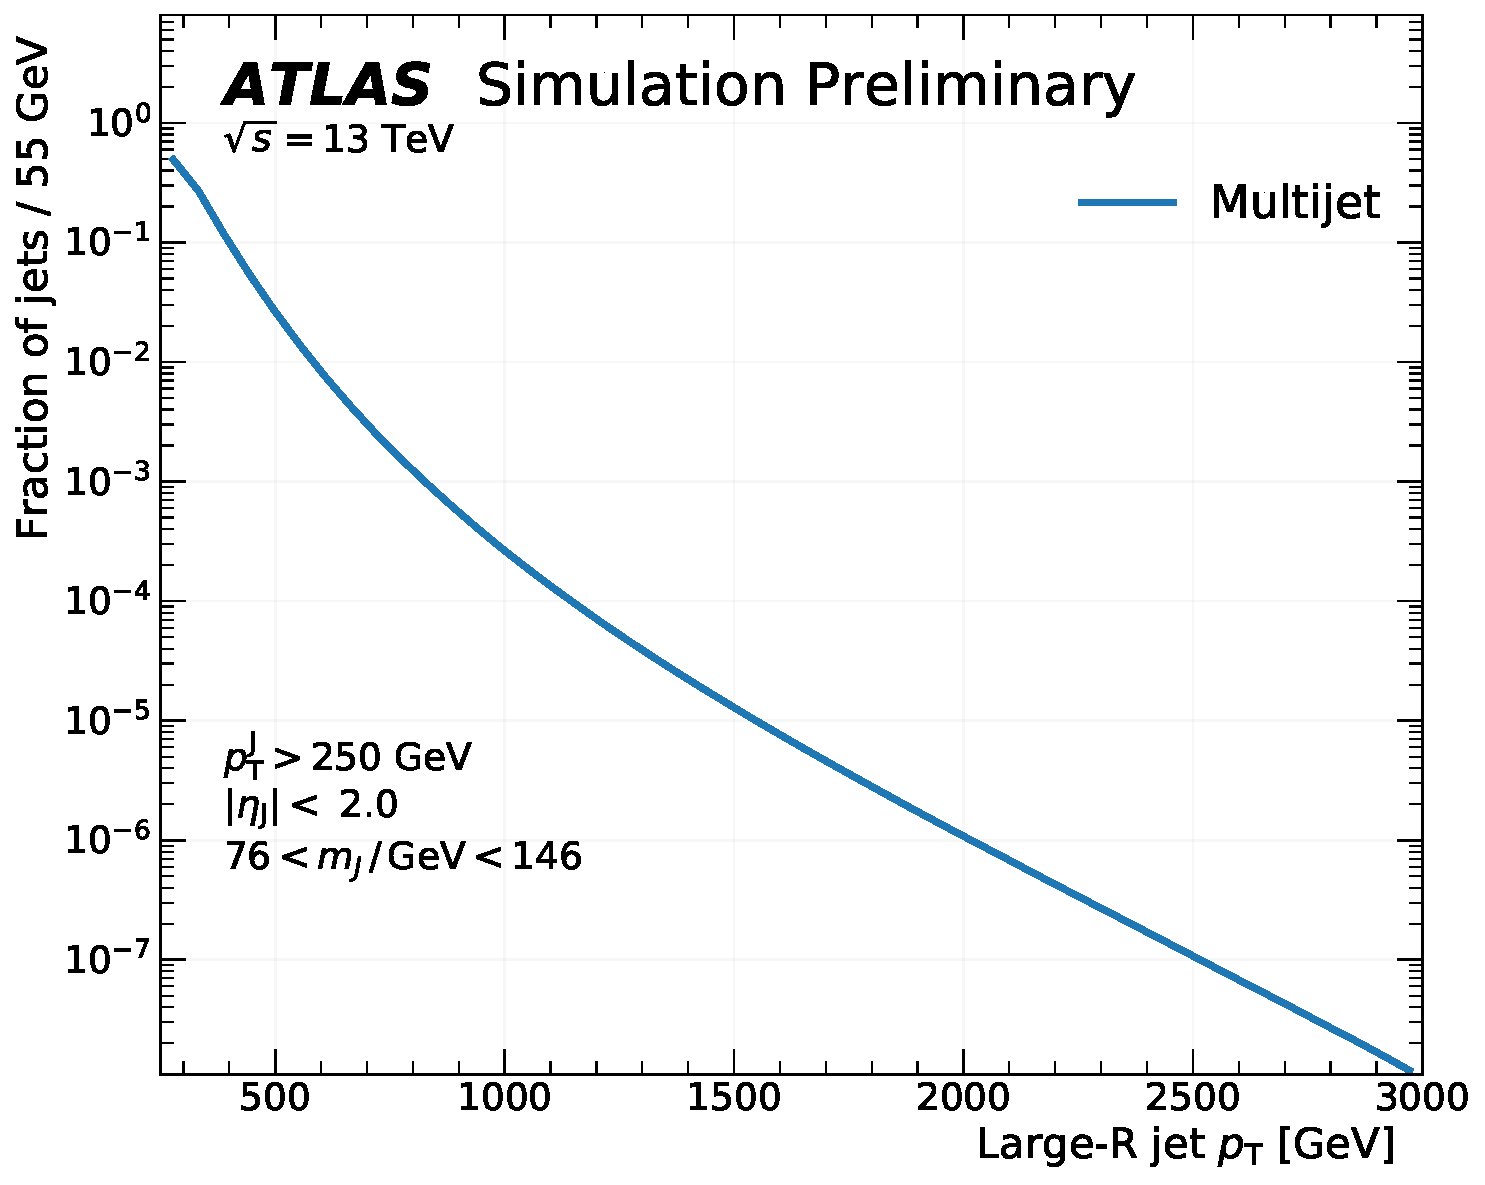
\includegraphics[width=0.75\textwidth]{figuresXbb/samples/pt_norm.pdf}
  \end{center}
  \caption{
  Multijet样本中领头LR-jet的横动量分布。分布已经归一化。
  }
    \label{fig:bkg-pt}
\end{figure}

所有信号和本底样本中的堆积事例都是用\textsc{Pythia 8}模拟实现的,
b强子和c强子衰变的建模
%是用
由\textsc{Evtgen}~\cite{Lange:2001uf}完成,
并且所有事例都会经过ATLAS探测器的全模拟过程进行处理~\cite{SOFT-2010-01,ATHENA}。
%而且它们都会经过一个全模拟过程来模拟事例在ATLAS探测器中的行为~\cite{SOFT-2010-01,ATHENA}。



\section{事例重建和筛选}
\label{sec:XbbOR}

%算法设计的目的是为了在不引入质量关联性的同时,
%提高来自高横动量$H\rightarrow b\bar{b}$事例与来自QCD过程的multijet事例和来自强子型衰变的t夸克事例的区分度。
事例的重建分为三步:
第一步是重建距离参数R=1的LR-jet,
%这是为了
%目的是
这样可以俘获整个大质量粒子的衰变,比如希格斯玻色子、t夸克;
第二步是重建LR-jet中的subjet,目的是
%为了
分辨和识别由大质量粒子衰变而来的
产物,
%夸克或胶子
%小质量粒子,
比如识别由希格斯玻色子衰变而来的b夸克;
第三步是将LR-jet与subjet进行有效的匹配。

\subsection{LR-jet的重建和筛选}
\label{sec:XbbORLR}

%在LR-jet的重建当中,
对于LR-jet的重建,
如第~\ref{sec:JET}~小节所述,首先重建量能器单元中具有噪声抑制功能的拓扑集群,
%~\cite{PERF-2014-07},
然后用anti-$k_t$算法
%~\cite{Cacciari:2008gp}
将这些拓扑集群重建为距离参数R=1的LR-jet,
接着
%利用
通过“幻影”关联
%算法~\cite{Cacciari:2008gn}
将内部探测器中径迹与LR-jet匹配起来。
随后通过修剪技术~\cite{Krohn:2009th}消除堆积事例和潜在事例的影响,
%具体来说,
在这个修剪过程中,
先使用距离参数R=0.2的$k_t$算法~\cite{KTA}重建LR-jet中可能的subjet,
对每个subjet,
%并
判断它携带的横动量是否小于LR-jet横动量的5\%,
如果小于,则将这个subjet从LR-jet中移除。
%如果这些subjet所携带的横动量小于LR-jet横动量的5\%,则将它们从这个LR-jet中移除。

为了克服量能器有限的角分辨率,合作组用一种独立的方法来评估LR-jet的质量~\cite{TAGGING5},
首先定义量能器质量$m^{calo}$和径迹质量$m^{track}$:
\begin{equation} 
\label{eq:LRMASS1}
 \begin{split}
  m^{calo}&=\sqrt{(\sum_{i\in  calo} E_i )^2-(\sum_{i\in calo} \vec{p}_i)^2}
  \\
  m^{track}&=\sqrt{(\sum_{i\in tracks} E_i )^2-(\sum_{i\in tracks} \vec{p}_i)^2}
 \end{split}
\end{equation}
其中$m^{calo}$和$m^{track}$中的$(E_i,\vec{p}_i)$分别是与LR-jet关联的量能器拓扑集群和带电粒子径迹的能量、动量,
在$m^{track}$的定义中径迹的质量设为$\pi$介子的质量。
%通过
结合与LR-jet关联的量能器拓扑集群和带电粒子径迹,
%的信息,
%可以
定义
一个
%一种
径迹关联质量$m^{TA}$,即这里所使用的LR-jet质量:
\begin{equation} 
\label{eq:LRMASS2}
 \begin{split}
m^{TA}&=\frac{p_{T}^{calo}}{p_{T}^{track}} \times m^{track},
\\
p_{T}^{track}&=\sum_{i\in tracks} \vec{p}_T^i, \quad p_{T}^{calo}=\sum_{i\in calo} \vec{p}_T^i
 \end{split}
\end{equation}
其中
%$m^{track}$是由径迹信息得到的质量,
$p_{T}^{calo}$是与LR-jet关联的拓扑集群的横动量的矢量和,
$p_{T}^{track}$ 是与LR-jet关联的径迹的横动量的矢量和。
比率$p_{T}^{calo}/p_{T}^{track}$可以修正来自LR-jet中
%不带电
中性
成分的贡献,从而提高LR-jet质量的分辨率。
图~\ref{fig:LRMASS}~展示了利用
%以上
上述
三种方式重建出来的LR-jet质量分布在校准前和校准后的对比,
虚线代表校准前的分布,实线代表校准后的分布,黑线代表$m^{TA}$,红线代表$m^{calo}$,蓝线代表$m^{track}$,
从峰值位置和宽度可以看出由$m^{TA}$重建出来的LR-jet更接近真实的分布。

最后会对LR-jet的能量和质量进行校准,以解决MC模拟中建模偏差~\cite{JETM-2018-02}。
%最后使用从MC模拟得到的校准因子将LR-jet的能量和质量校准到粒子水平~\cite{JETM-2018-02}。
重建和校准完成之后,
领头LR-jet满足如下筛选条件的
事例将会用于后续分析:$p_{T}$>250GeV、$p_{T}$<3000GeV和$|\eta|$<2.0。


\begin{figure}
  \begin{center}
    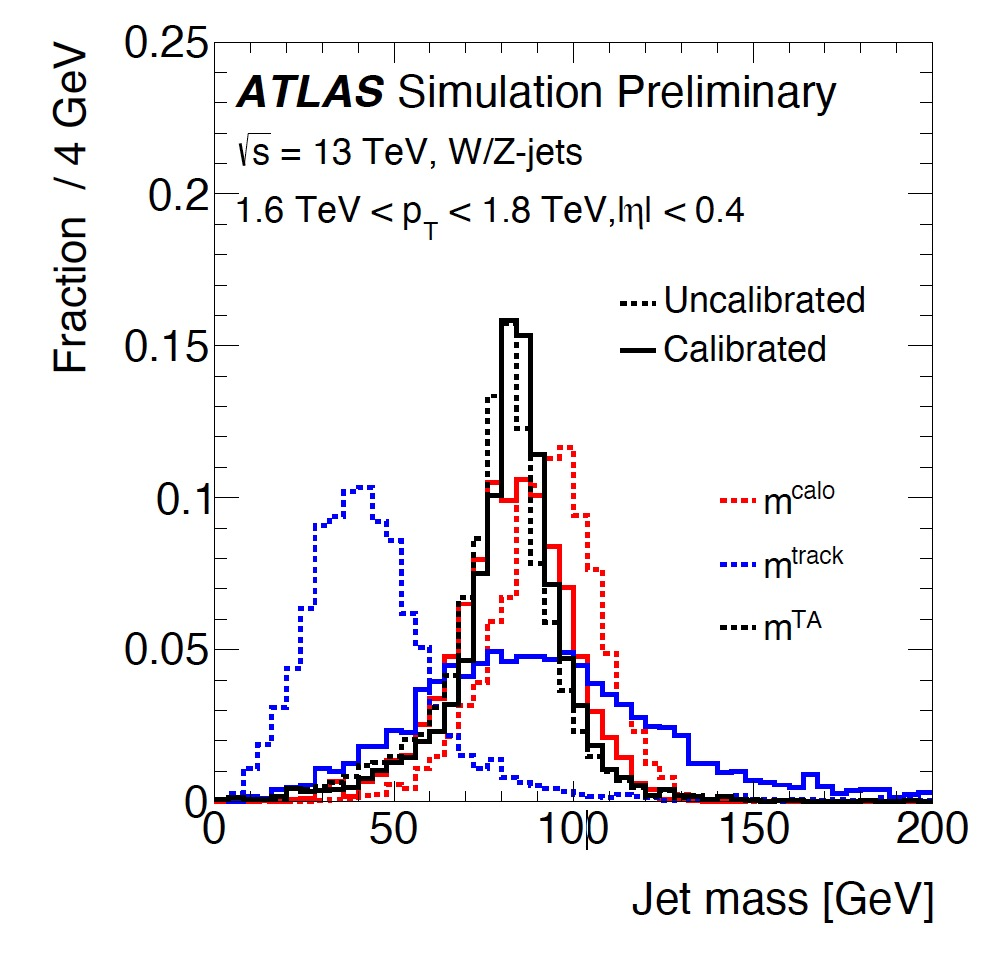
\includegraphics[width=0.75\textwidth]{figuresXbb/LRMASS.jpg}
  \end{center}
  \caption{
  通过量能器质量$m^{calo}$、径迹质量$m^{track}$和径迹关联质量$m^{TA}$三种方式重建出来的LR-jet分布在校准前后的对比。
  虚线代表校准前的分布,实线代表校准后的分布,黑线代表$m^{TA}$,红线代表$m^{calo}$,蓝线代表$m^{track}$。
  }
    \label{fig:LRMASS}
\end{figure}



\subsection{subjet的重建和筛选}
\label{sec:XbbORSR}

%而在LR-jet中subjet的重建过程中,
对于LR-jet中subjet的重建,
%合作组
最初是
%通过
基于内部探测器中的径迹
%重建出来的
~\cite{TAGGING1,TAGGING5},
与第~\ref{sec:JET}~小节中做法不同的是,
基于径迹的重建算法是
%subjet是直接
以内部探测器中径迹为单元,
固定距离参数R=0.2,用anti-$k_t$算法将这些径迹
会聚成subjet,
%聚集并重建出来的,
记为FR-jet。

当希格斯玻色子的横动量没有足够高时,FR-jet算法能非常有效的重建其中的b-jet,
%在希格斯玻色子的横动量没有足够高到使得衰变而来的两个b-jet重叠之前,FR-jet算法能非常有效的重建subjet,
但是,当横动量足够高
%并使
到使得衰变而来的两个b-jet重叠的时候,FR-jet算法便不能分辨这两个b-jet了,
为了解决这个问题,在2017年经过性能优化之后,
合作组引入了一种距离参数R可变的subjet重建算法~\cite{VRJET1,VRJET2},记为VR-jet,
在这个算法中,距离参数R是subjet横动量$p_T$的函数:
\begin{equation} 
\label{eq:VR}
R_{eff}(p_{T})=\frac{\rho}{p_T}
\end{equation}
%其中新参数$\rho$决定了有效的subjet尺寸大小随着这个subjet横动量动量减小的速度。
其中参数$\rho$决定了subjet的有效尺寸随着横动量减小的速度。
为了使b强子方向与subjet轴向
%之间
的匹配效率最大化,
这个参数固定为$\rho=30GeV$,
%这个常数$\rho=30GeV$,
在使用anti-$k_t$算法将径迹和VR-jet匹配的过程中,
有效距离参数$R_{eff}$会随着subjet横动量的增大而减小,
从而使低横动量subjet的缔合锥(Association cone)更宽,高横动量subjet的缔合锥体更窄。
%除了之外,
另外,为了防止subjet在低横动量时变得太大或者在高横动量时收缩到探测器分辨率以下,
%这个
算法还引入了两个参数分别是subjet尺寸的上限$R_{\text{min}}=0.02$和下限$R_{\text{min}}=0.4$。
%该算法还有两个附加的参数分别是subjet大小的上限$R_{\text{min}}=0.02$和下限$R_{\text{min}}=0.4$,
%这个限制可以防止jet在低横动量时变得太大或者在高横动量时收缩到探测器分辨率以下。

%与此同时,
上述两种subjet重建算法中
都包含以下对径迹的筛选要求:
$p_{T}>0.5GeV$和$|\eta|<2.5$;
%而且
其在
PD
%像素探测器
和
SCT
%半导体径迹探测器
上至少留下七个探测点(Hits);
PD
%像素探测器
上最多缺少一个预期的探测点,
%半导体径迹探测器
SCT
上最多缺少两个预期的探测点,并且与其他径迹最多共享一个探测点,
这些筛选要求可以大大的减少来自堆积事例的径迹。
随后,
%为了更完整收集用于b-jet标定算法实现的径迹,
为了更完整的收集b-jet标定算法用到的径迹,
会将
不满足上述筛选条件
%其他满足更宽松的筛选条件
的径迹与subjet进行匹配~\cite{TRAVR},
匹配过程是基于subjet轴线与径迹之间的角距
$\Delta R$\footnote{如式~\ref{eq:DRdef}~所示,角距$\Delta R$定义为两个物理对象在$\eta$-$\phi$平面内的距离。}
,其阈值也会随着subjet横动量的增大而减小,
从而使得低横动量subjet的缔合锥更宽,高横动量subjet的缔合锥体更窄,准直性更好,
一个径迹最多与一个subjet匹配,当多个subjet满足要求时,选取$\Delta R$最小的那个subjet进行匹配。
%subjet重建完成之后,
最后,要求其重建好的subjet满足$p_{T}$>7GeV和$|\eta|$<2.5,且至少有两条与之关联的径迹。

%如
图~\ref{fig:ATLASJET2}~展示了利用FR-jet和VR-jet算法重建LR-jet中的subjet的对比示意图,
可以看到,当两个b-jet快要重叠时,VR-jet对它们的分辨率更好。
其中VR-jet是本章第~\ref{sec:XbbTagger}~小节中用于高横动量
$H\rightarrow b\bar{b}$
%LR-jet
标定算法的开发和研究的
基础
%基本
%subjet重建
算法,
另一种
%subjet重建
算法FR-jet也会用于第~\ref{sec:XbbPerf}~小节中算法性能的对比。
%当中。

\begin{figure}
  \begin{center}
    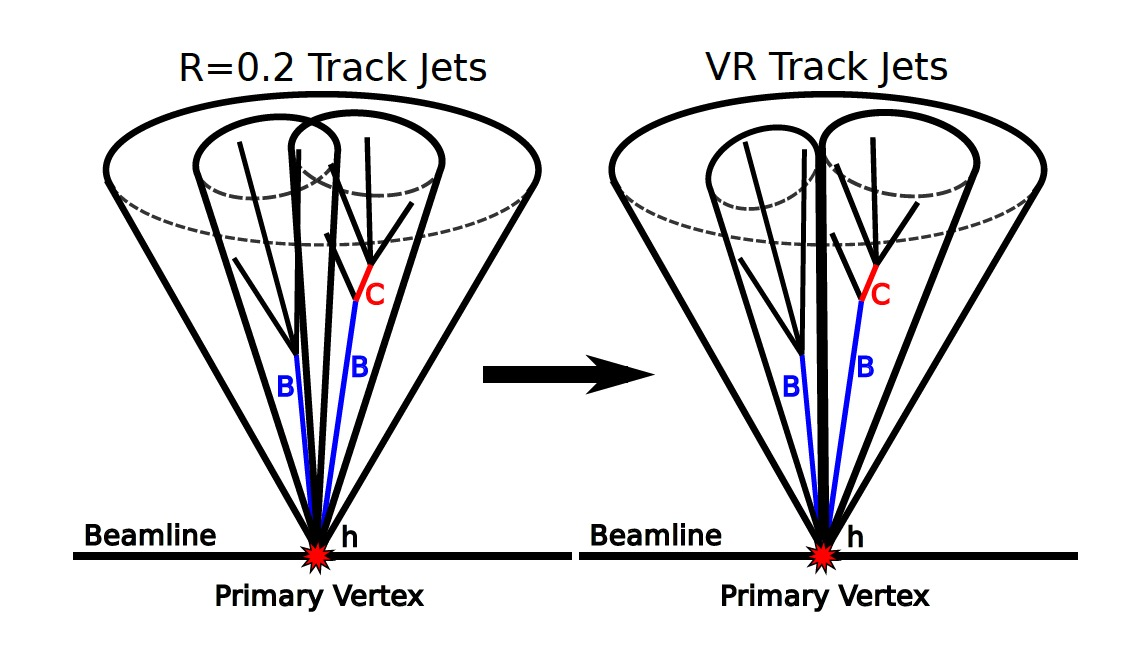
\includegraphics[width=0.9\textwidth]{figuresEXP/ATLASJET2.jpg}
  \end{center}
  \caption{
利用FR-jet(左图)和VR-jet(右图)算法重建LR-jet中subjet的对比示意图。
  }
    \label{fig:ATLASJET2}
\end{figure}


\subsection{味标签}
\label{sec:XbbORFT}

%在MC样本中,
样本中FR-jet和VR-jet的真实味标签是通过与产生子层面的真实强子进行几何匹配来确定的。
基于事例中b强子或c强子与subjet轴线之间的角距$\Delta R$
%\footnote{如式~\ref{eq:DRdef}~所示,角距$\Delta R$定义为两个物理对象在$\eta$-$\phi$平面内的距离。}
:如果在$\Delta R$<0.3的范围内有一个b强子,那么这个subjet会被标签为b-jet,
若是按这种方式一个b强子可以匹配多个subjet,那么只有与这个b强子最接近的subjet才会被标签为b-jet;
如果在$\Delta R$<0.3的范围内没有b强子但是有一个c强子,那么这个subjet会被标签为c-jet,
同样当一个c强子可以匹配多个subjet时,只有与这个c强子最接近的subjet才会被标签为c-jet;
如果在$\Delta R$<0.3的范围内即没有b强子也没有c强子,那么将这个subjet标签为light-jet。

给LR-jet贴上正确的味标签对于后续
%分析
标定算法的性能分析
%信号效率和本底排除率来说
至关重要,
它是通过
%其
与真实jet之间的匹配实现的,这里将真实jet记为TH-jet。
在MC样本中,TH-jet是通过产生子层面的真实粒子构建的,
为了与探测器响应相对应,要求这些真实粒子的寿命大于10ps,且不包含$\mu$和中微子,
随后以这些真实粒子的径迹为单元,
用anti-$k_t$算法将这些径迹重建为距离参数R=1的TH-jet,
再利用角距匹配将TH-jet和真实的希格斯玻色子或者t夸克对应起来。
%使用第~\ref{sec:JET}~小节中与LR-jet重建相同的重建算法构建TH-jet。
有了TH-jet之后,基于事例中TH-jet轴线与LR-jet轴线之间的角距$\Delta R$给LR-jet贴上真实的味标签:
如果在$\Delta R$<1的范围内有一个来自希格斯玻色子的TH-jet,并且TH-jet中还包含两个b强子,
那么这个LR-jet会被标签为来自希格斯玻色子的LR-jet,记为Higgs-jet,
若是按这种方式一个TH-jet可以匹配多个LR-jet,那么只有与这个TH-jet最接近的LR-jet才会被标签为Higgs-jet;
如果在$\Delta R$<1的范围内有一个来自t夸克的TH-jet,
那么这个LR-jet会被标签为来t夸克的LR-jet,记为Top-jet,
同样当一个TH-jet可以匹配多个LR-jet,只有与这个TH-jet最接近的LR-jet才会被标签为Top-jet;
其余的LR-jet都被标签为QCD-jet。
对于信号样本,要求事例中至少包含一个Higgs-jet,
%而
对于t夸克样本,要求事例中至少包含一个Top-jet。

\subsection{LR-jet与subjet的匹配}
\label{sec:XbbORMT}

%在subjet和LR-jet
重建完成之后,便是subjet
%即FR-jet或VR-jet
与LR-jet之间的匹配,
它也是通过“幻影”关联的算法
%~\cite{Cacciari:2008gn}
实现的,在第~\ref{sec:JET}~小节有该算法的简要描述。
与简单的角距匹配相比,“幻影”关联算法的匹配功能更强大,
它可以实现具有不规则边界的jet之间的匹配。
%首先,“幻影”是指事例中subjet横动量被设置成无穷小之后的四矢量,
%基本只保留了subjet的方向信息,
%然后用anti-$k_t$算法将这个“幻影”和构成LR-jet的量能器拓扑集群重新会聚成R=1的LR-jet,
%这样保证了重建出来的LR-jet仍然是未修建之前的LR-jet,
%如果此时“幻影”也是LR-jet的组成部分,那么相应的subjet就和LR-jet匹配上了。


\subsection{b-jet标定算法}
\label{sec:XbbORBJ}

如第~\ref{sec:BJET}~小节
所述,
%所描述的,
对于subjet,
这里使用的b-jet标定算法有MV2和DL1r,这也是ATLAS合作组在上一轮和目前推荐的算法,
%常用的b-jet标定算法有MV2和DL1r两种~\cite{ATL-PHYS-PUB-2017-013,DLOR1,DLOR2},
它们都是%基于
利用
一些低级算法
%利用机器学习
发展
%出来
而来
的高级算法,其中低级算法是利用b-jet独特的性质构建起来的,
MV2基于提升决策树,DL1r基于神经网络。
%MV2以提升决策树为框架,而DL1r以深度学习神经网络为框架。
图~\ref{fig:VRDL1r}~展示的是对于MV2、DL1和DL1r三种算法,
利用VR-jet重建的subjet中
%VR-jet中
b-jet标定效率与c-jet
排除率和light-jet排除率的关系~\cite{DLOR2},
可以看到DL1r的性能更优于MV2,
因此,DL1r算法将会用与后续高横动量$H\rightarrow b\bar{b}$标定算法的开发,
而MV2和DL1r都将用作基线算法来研究
%高横动量$H\rightarrow b\bar{b}$标定算法
这个新算法的
的性能。

\begin{figure}  
  \begin{center}
    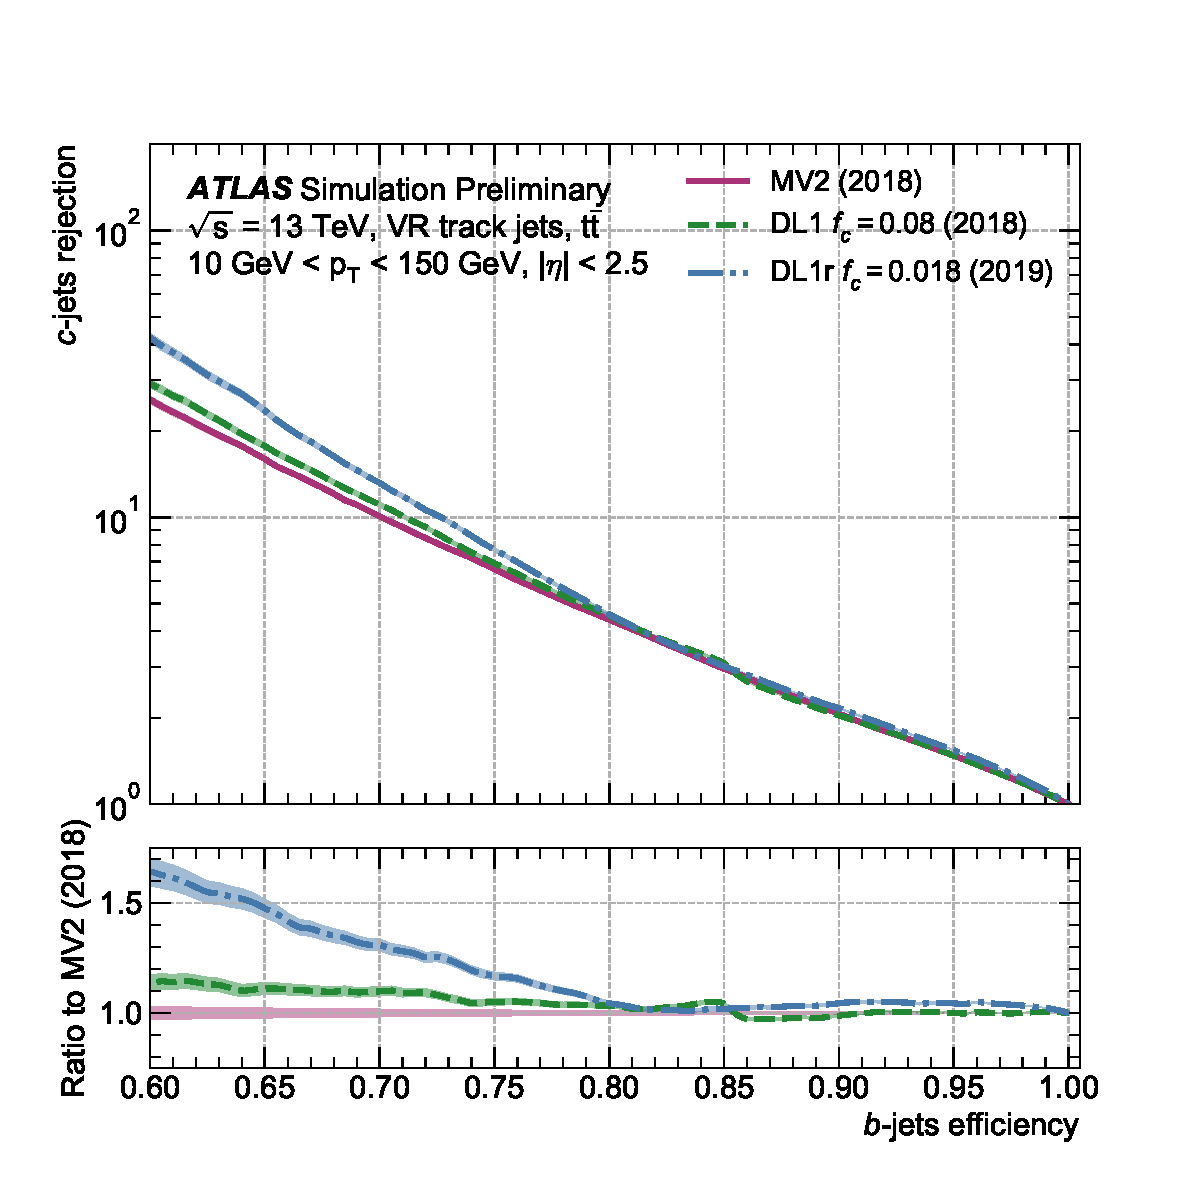
\includegraphics[width=0.45\textwidth]{figuresXbb/VRDL1r2.pdf}
    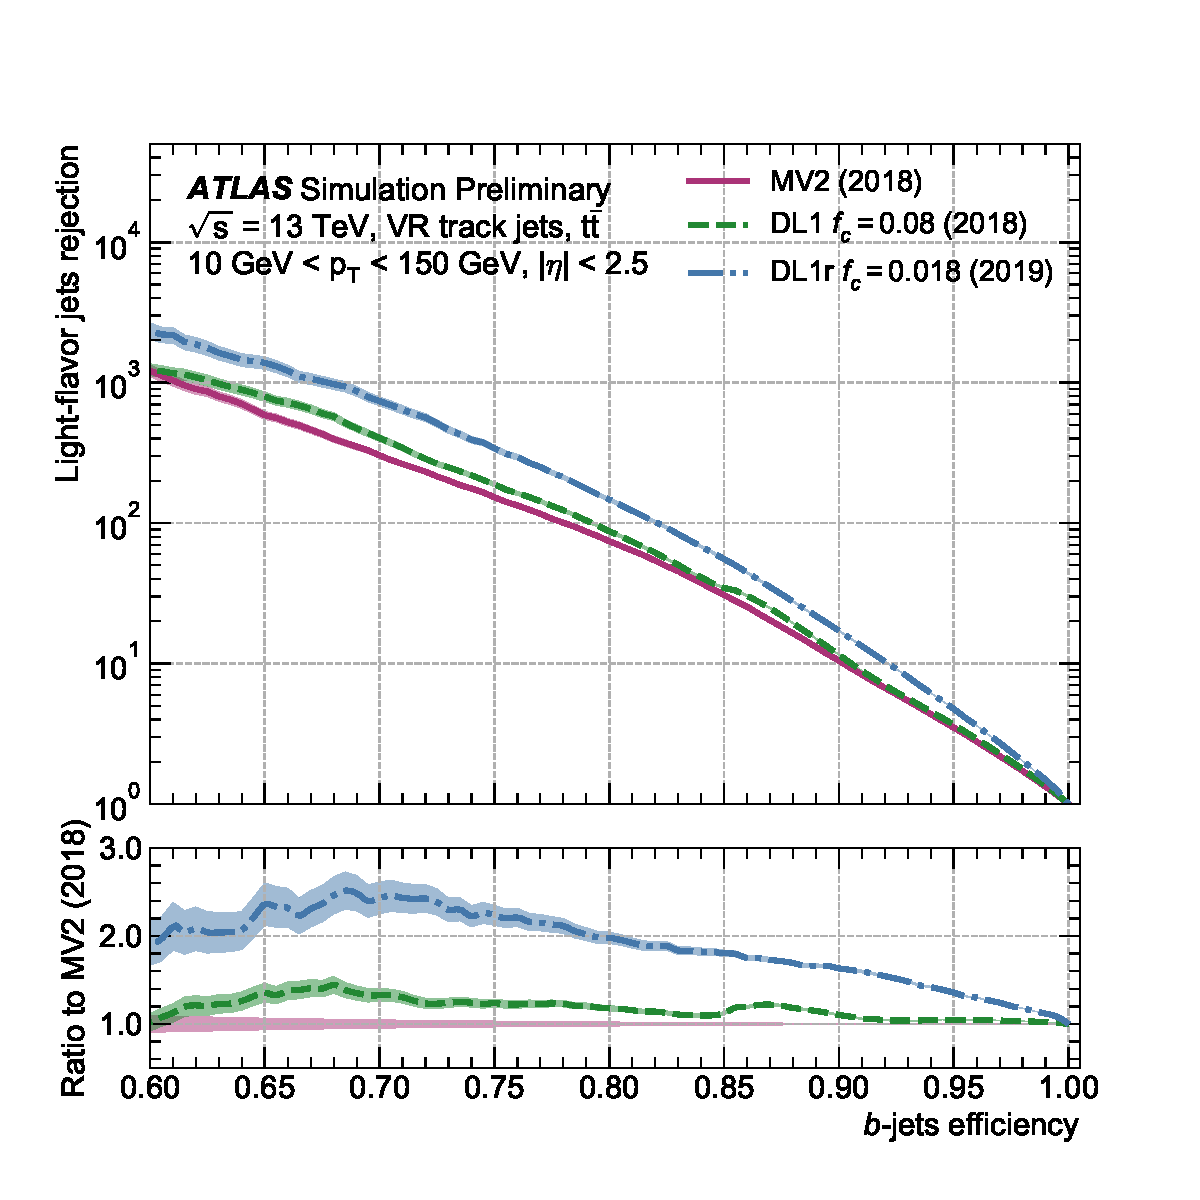
\includegraphics[width=0.45\textwidth]{figuresXbb/VRDL1r1.pdf}
  \end{center}
  \caption{
 对于MV2、DL1和DL1r三种算法,
利用VR-jet重建的subjet中
%VR-jet中
b-jet标定效率与c-jet
排除率和light-jet排除率的关系。
 % 对于MV2、DL1和DL1r三种b-jet算法,VR-jet中b-jet标定效率与c-jet排除率(左图)和light-jet排除率(右图)的关系。
   }
  \label{fig:VRDL1r}
\end{figure}

\subsection{LR-jet的结构变量}
\label{sec:XbbORJSS}


前面提到,
合作组引入了一部分用于高横动量
%的
W玻色子和t夸克标定的LR-jet的结构变量,
用来研究高横动量$H\rightarrow b\bar{b}$的标定算法。
如表~\ref{tab:JS}~所示,在新算法的研究和设计过程中,
我们
%利用
使用
了这14个典型的结构变量,
这里将做简要介绍。
%这里做简要介绍。

\begin{table}[ht]
\caption{用于高横动量$H\rightarrow b\bar{b}$标定算法的研究和设计的部分LR-jet结构变量。}
\begin{center}
\begin{adjustbox}{width=\columnwidth,center}
\begin{tabular}{c|c|c}
    \hline
    \hline
    Observable & Variable & Tagging and reference \\
    \hline  
    Energy correlation ratios & $C_2,D_2,e_3$ & t,W\cite{JSS1,JSS2} \\
    \hline  
    N-subjettiness & $\tau_{21},\tau_{32}$ & t,W\cite{JSS3,JSS4} \\
    \hline  
    KtDR & $KtDR$ & W\cite{JSS14} \\
    \hline  
    Qw & $Q_w$ & W\cite{JSS8} \\
    \hline  
    Splitting Measures & $Z_{CUT12},\sqrt{d_{12}},\sqrt{d_{23}}$ & t,w\cite{JSS8,JSS10} \\ 
    \hline  
    Center of mass observables & Fox Wolfram($R_2^{FW}$) & W\cite{JSS5}  \\
    \hline  
    Aplanarity & $A$ & W\cite{JSS6} \\
     \hline  
    Angularity & $a_3$ & W\cite{JSS13} \\
    \hline  
    Planar Flow & $\mathcal{P}$& W\cite{JSS11} \\
    \hline
    \hline
\end{tabular}
\end{adjustbox}
\end{center}
\label{tab:JS}
\end{table}

第一组变量是LR-jet的能量关联比,
为了表征LR-jet内部的辐射结构,
利用LR-jet组成成分的能量和相对角距,
研究~\cite{JSS1,JSS2}引入了一般性的能量关联函数:
\begin{equation} 
\label{eq:JSS1}
 \begin{split}
E_{CF1}&=\sum_{i\in J} p_{T}^i
\\
E_{CF2}(\beta)&=\sum_{i<j\in J} p_T^i p_T^j (R_{ij})^\beta
 \\
E_{CF3}(\beta)&=\sum_{i<j<k\in J} p_T^i p_T^j (R_{ij})^\beta
 \end{split}
\end{equation}
其中i、j、k是LR-jet的组份,$p_{T}^i$是第i个组份的横动量,
$R_{ij}$是第i个组份与第j个组份之间的角距,
$\beta$取正整数,用于给组份的角距加权。
接着可以定义两组比率:
\begin{equation} 
\label{eq:JSS2}
 \begin{split}
e_2^{(\beta)}&=\frac{E_{CF2}(\beta)}{E_{CF1}^2}
\\
e_3^{(\beta)}&=\frac{E_{CF3}(\beta)}{E_{CF1}^3}
 \end{split}
\end{equation}
然后可以更近一步的定义:
\begin{equation} 
\label{eq:JSS3}
 \begin{split}
C_2^{(\beta)}&=\frac{e_3^{(\beta)}}{(e_2^{(\beta)})^2}
\\
D_2^{(\beta)}&=\frac{e_3^{(\beta)}}{(e_2^{(\beta)})^3}
 \end{split}
\end{equation}
研究表明它们对于LR-jet内部结构的识别有一定
作用,
%用处,
其中$e_3=e_3^{(\beta=1)}$、$C_2=C_2^{(\beta=1)}$和$D_2=D_2^{(\beta=1)}$
在W玻色子标定和t夸克标定中都表现出一定的区分能力~\cite{JSCD2}。

第二组变量用于表征LR-jet中的subjet多样性~\cite{JSS3,JSS4},
基于$k_t$算法~\cite{JSS14,JSTAU},可以将LR-jet的组份会聚成N个subjet,
然后可以定义一个变量$\tau_N$,用于量化这N个subjet能够多么合适的描述LR-jet:
\begin{equation} 
\label{eq:JSS4}
\tau_N = \frac{ \sum_{i\in J} p_T^i min \{ \Delta R_{1i},R_{2i},\dots ,R_{Ni} \} }{R\sum_{i\in J} p_T^i}
\end{equation}
其中$p_T^i$是第i个组份的横动量,
$min \{ \Delta R_{1i},R_{2i},\dots ,R_{Ni}, \}$是第i个组份与距离这个组份最近的subjet轴线的角距,
R=1是LR-jet的距离参数。
当$\tau_N \approx 0$时,表明LR-jet中的每个组份都有与之共线的subjet相对应,
%而
当$\tau_N \approx 1$时,表明在
%除了
靠近subjet轴线外的其他方向仍有显著的能量辐射,
也就是这N个subjet不能合适的描述这个LR-jet。
为了区分两体衰变和三体衰变,
引入比率$\tau_{21}=\tau_2/\tau_1$和$\tau_{32}=\tau_3/\tau_2$,
它们在W玻色子标定和t夸克标定中也表现出一定的区分能力~\cite{JSS3}。

第三组变量KtDR也是基于对LR-jet组份
%进行
的
重新会聚,
在距离参数R=0.4的情况下可以通过$k_t$算法将LR-jet的组份会聚成两个subjet,
而变量KtDR便是这两个subjet轴线之间的角距~\cite{JSS14}。
对于%LR-jet
质量为m横动量为$p_T$的LR-jet的两体衰变,
这个变量有一个特征值$KtDR\approx 2m/p_T$。

第四组变量Qw同样是基于对LR-jet组份
%进行
的重新会聚,
%也可以
通过$k_t$算法将LR-jet的组份会聚成三个subjet,
变量$Q_w$表示其中两个subjet的不变质量最小的值~\cite{JSS8}。
它是针对三体衰变过程优化的变量,
在由t夸克衰变而来的W玻色子的标定中有一定的作用。

第五组变量是基于$k_t$算法在会聚LR-jet组份过程中所形成的中间
%过程
subjet,
定义两个与式~\ref{eq:TOPOSN}~类似的分离比例$\sqrt{d_{12}}$和$\sqrt{d_{23}}$~\cite{JSS10}:
\begin{equation} 
\label{eq:JSS45}
\sqrt{d_{ij}}=min(p_T^i,p_T^j)\Delta R_{ij}
\end{equation}
$\sqrt{d_{12}}$代表$k_t$算法在最后一步合并过程中从2个subjet到1个subjet的分离比例,
$\sqrt{d_{23}}$代表$k_t$算法在倒数第二步合并过程中从3个subjet到2个subjet的的分离比例。
其中$p_T^i$是利用$k_t$算法会聚过程中的第i个subjet的横动量,
是$\Delta R_{ij}$第i个subjet和第j个subjet的角距。
对于高横动量强子型衰变的t夸克,
$\sqrt{d_{12}}$的期望值约为t夸克质量的一半$m_t/2$,
对于高横动量强子型衰变的W玻色子,
$\sqrt{d_{23}}$的期望值约为W玻色子质量的一半$m_W/2$。
但是对于来自QCD过程的轻夸克或者胶子辐射,
分离比例$\sqrt{d_{12}}$和$\sqrt{d_{23}}$都较小~\cite{JSD12}。
在此基础上可以定义一个与分离比例相关的变量~\cite{JSS8}:
\begin{equation} 
\label{eq:JSS46}
Z_{cut12}=\frac{d_{12}}{d_{12}+m^2}
\end{equation}
其中$d_{12}$是式~\ref{eq:JSS45}~中定义的最后一步合并过程中的分离比例,
m是最后一步合并过程中由第1个和第2个subjet重新会聚而成的subjet的质量。
对于两体衰变,m代表LR-jet的质量,
$Z_{cut12}$也是和$d_{12}$类似的子结构变量,
但是通过对m进行归一化,可以减少它对LR-jet质量的依赖性。


第六组变量是二阶与零阶Fox-Wolfram矩的比率~\cite{JSS5},
最开始提出的Fox-Wolfram矩是用来表征正负电子碰撞事例的形状,
随后也用来研究LR-jet的形状,
它是在LR-jet的质心系下定义的,
首先将LR-jet的组份利用洛伦兹变换提升到质心系:
\begin{equation} 
\label{eq:JSS5}
 \begin{split}
 \tilde{E}&=\gamma(E+\vec{\beta}\cdot \vec{p})
\\
\tilde{\vec{p}}&=\vec{p}+\frac{\gamma-1}{|\vec{\beta}|^2} (\vec{\beta}\cdot \vec{p}) \vec{\beta}+\gamma E\vec{\beta}
 \end{split}
\end{equation}
其中$\vec{\beta}=\vec{p}_J/E_J$是LR-jet的速度矢量与真空光速的比值,
$\gamma$是洛伦兹变换因子。
接下来可以在质心系下定义l阶Fox-Wolfram矩:
\begin{equation} 
\label{eq:JSS6}
H_l=\sum_{1\le i<j\le n_J} \frac{|\tilde{\vec{p_i}}| |\tilde{\vec{p_j}}|}{s} P_l (\cos \theta_{ij})
\end{equation}
其中$\tilde{\vec{p_i}}$是LR-jet第i个组份的动量,
$s=(\sum_i E_i)^2$是组份的能量和的平方,
$P_l$是第l阶勒让德多项式,
$\theta_{ij}$是第i个组份与第j个组份之间的夹角,
上述与LR-jet组份相关的变量都是质心系下的变量。
随后可以定义归一化的二阶Fox-Wolfram矩,即二阶与零阶Fox-Wolfram矩的比率:
\begin{equation} 
\label{eq:JSS61}
R_2^{FW}=\frac{H_2}{H_0}=\frac{\sum_{1\le i<j\le n_J} |\tilde{\vec{p_i}}| |\tilde{\vec{p_j}}|  (3\cos^2 \theta_{ij}-1 )/2 }
{\sum_{1\le i<j\le n_J} |\tilde{\vec{p_i}}| |\tilde{\vec{p_j}}|}
\end{equation}
归一化的二阶Fox-Wolfram矩对在质心系下对称的结构即背对背的辐射结构比较敏感,
使得它可以用于区分两体衰变和三体衰变。

第七组变量平面度A也是一个形状变量,
它也是在LR-jet的质心系下定义的~\cite{JSS6},
将LR-jet的组份利用洛伦兹变换~\ref{eq:JSS5}~提升到质心系之后,
首先定义一个$3\times 3$的球形矩阵:
\begin{equation} 
\label{eq:JSS62}
S^{k,l}=\frac{ \sum_{1\le i<j\le n_J} \tilde{p}_i^k  \tilde{p}_j^l  }
{\sum_{i=1}^{n_J} |\tilde{\vec{p}}_i|^2}
,\quad k,l \in \{x,y,z\}
\end{equation}
其中$n_J$是LR-jet的组份数量,$\tilde{\vec{p}}_i$是第i个组份的动量,
$\tilde{p}_j^l$和$\tilde{p}_i^k$是第i个组份的动量分量,
上述与LR-jet组份相关的变量都是质心系下的变量。
这个球形矩阵$S^{k,l}$有三个本征值$\lambda_1\le \lambda_2\le \lambda_3$,它们的和为1,
利用本征值$\lambda_3$可以定义平面度:
\begin{equation} 
\label{eq:JSS63}
A=\frac{3\lambda_3}{2}
\end{equation}
它满足$0\le A \le 1/2$,
在质心系下,对于QCD过程中轻夸克或胶子各向同性的弥散辐射,$A\approx 1/2$,
对于背对背的两体衰变,%会使得
$A \approx 0$。


第八组变量倾斜度$a_3$由以下式子定义~\cite{JSS13,JSA3}:
\begin{equation} 
\label{eq:JSS7}
a_3=\frac{1}{m_J} \sum_{i=1}^{n_J} E_i \sin^{-2} \theta_i (1-\cos \theta_i)^3
\end{equation}
其中$m_J$为LR-jet的质量,$n_J$是其组份数量,
$E_i$是第i个组份的能量,$\theta_i$是第i个组份相对于LR-jet轴线的夹角。
$a_3$测量了广角辐射在LR-jet中所占的比重。
对于对称的两体衰变,$a_3$趋向于较小的值,
对于
QCD过程中
%非共振态的
轻夸克或者胶子辐射,$a_3$趋向于较大的值。

%\mathbf
第九组变量平面流$\mathcal{P}$用于衡量LR-jet中能量
在垂直于其轴线方向的平面上的分布,
以及沿平行于其轴线方向的分布情况~\cite{JSS11}。
%沿垂直于其轴线方向的平面和平行于其轴线方向的分布情况~\cite{JSS11}。
将LR-jet动量$\vec{P}$以及其组份的动量$\vec{p}_i$先绕z轴旋转$-\phi$:
\begin{equation} 
\label{eq:JSS8}
\mathbf{R}_{\phi}=
\begin{bmatrix}
\cos \phi & \sin\phi & 0\\
-\sin\phi & \cos\phi & 0\\
 0&0&1
\end{bmatrix}
\end{equation}
然后再绕y轴旋转$-\theta$:
\begin{equation} 
\label{eq:JSS9}
\mathbf{R}_{\eta}=
\begin{bmatrix}
\cos \theta & 0 & -\sin\theta\\
0 & 1 & 0\\
 \sin\theta&0& \cos\theta
\end{bmatrix}
=
\begin{bmatrix}
\tanh\eta & 0 & -\sech\eta\\
0 & 1 & 0\\
 \sech\eta&0& \tanh\eta
\end{bmatrix}
\end{equation}
其中$\phi$和$\eta$分别是LR-jet轴线的方位角和赝快度。
两次旋转操作之后,%使得
LR-jet的动量方向会指向z轴正向:
\begin{equation} 
\label{eq:JSS10}
\tilde{\vec{P}}=\mathbf{R}_{\eta}\mathbf{R}_{\phi}\vec{P}=
\begin{bmatrix}
\tanh\eta\cos \phi & \tanh\eta\sin\phi & -\sech\eta\\
-\sin\phi & \cos\phi & 0\\
  \sech\eta\cos\phi &\sech\eta\sin\phi & \tanh\eta
\end{bmatrix}
\begin{bmatrix}
P_x \\
P_y \\
P_z
\end{bmatrix}
=
\begin{bmatrix}
0 \\
0 \\
|\vec{P}|
\end{bmatrix}
\end{equation}
这样便于研究LR-jet组份的动量$\vec{p}_i$
%沿着
在垂直于LR-jet轴线方面的平面上的分布情况。
利用上述旋转矩阵将其组份i随着LR-jet轴线变换:
%之后:
\begin{equation} 
\label{eq:JSS11}
\tilde{\vec{p}}_i=\mathbf{R}_{\eta}\mathbf{R}_{\phi}\vec{p}_i
\end{equation}
其中$\vec{p}_i$是LR-jet第i个组份的动量,
接着可以定义一个$2\times 2$的动量矩阵$I_E$:
\begin{equation} 
\label{eq:JSS12}
I_E^{kl}=\frac{1}{m_J} \sum_{i=1}^{n_J} \frac{\tilde{p}_i^k\tilde{p}_i^l}{E_i}, \quad k,l \in \{x,y\}
\end{equation}
其中$m_J$是LR-jet的质量,$n_J$是其组份数量,
$E_i$是第i个组份的能量,$\tilde{p}_i^k$是第i个组份在旋转之后的动量分量。
随后平面流可以通过矩阵$I_E$的两个本征值$\lambda_1$和$\lambda_2$来定义:
\begin{equation} 
\label{eq:JSS13}
\mathcal{P}=\frac{3\det{I_E}}{tr(I_E)^2}=\frac{4\lambda_1\lambda_2}{(\lambda_1+\lambda_2)^2}
\end{equation}
如果能量在垂直于LR-jet轴线方向的平面上分布比较均匀,
会使$\lambda_1\approx\lambda_2\approx 1/2$,从而平面流$\mathcal{P}\approx 1$;
如果能量沿平行于LR-jet轴线的方向分布比较均匀,
则$\lambda_1\gg \lambda_2$,平面流$\mathcal{P}\approx 0$。
由于两体衰变趋向于产生沿着LR-jet轴线方面的线性能量分布,
而
%非共振态的
QCD过程中轻夸克或者胶子
%辐射
更趋向于产生
各向同性的弥散辐射,
%弥散的各向同性的能量辐射,
因此平面流$\mathcal{P}$
可以作为一个很好的区分变量。
%非常适合区分这两者。













































\section{高横动量$H\rightarrow b\bar{b}$标定算法}
\label{sec:XbbTagger}

%新算法设计是基于深度学习神经网络,其目的是为了在不引入质量关联性的同时,
%提高Higgs-jet与Top-jet或QCD-jet的区分能力。

新算法设计是基于%深度学习
神经网络,
%在第~\ref{cha:ML}~章有简要介绍神经网络。
%新算法
设计的目的是为了在不引入质量关联
%性
的同时,
提高来自高横动量$H\rightarrow b\bar{b}$事例与来自QCD过程的multijet事例和来自强子型衰变的t夸克事例的区分精度。
%其
神经网络的训练是在\textsc{Keras}~\cite{Chollet:2015}的框架下以\textsc{TensorFlow}~\cite{Tensorflow:2015}为平台完成的。
训练所用的结构参数如表~\ref{tab:Hyper}~所示,
%训练过程中,
为了防止过拟合(Overfitting),用于训练、验证和测试的样本是分开的,
其中用于训练的样本容量为$6\times 10^{6}$。
算法的输出有$p_{\text{Higgs}}$、$p_{\text{multijet}}$和$p_{\text{top}}$三个,
分别代表事例是来自Higgs-jet、QCD-jet和Top-jet事例的概率,
在这一小节的新算法开发过程所使用的区分因子
是$p_{\text{Higgs}}/p_{\text{multijet}}$和$p_{\text{Higgs}}/p_{\text{top}}$,
其中$p_{\text{Higgs}}/p_{\text{multijet}}$用来区分来自高横动量$H\rightarrow b\bar{b}$事例与来自QCD过程的multijet事例,
$p_{\text{Higgs}}/p_{\text{top}}$用来区分来自高横动量$H\rightarrow b\bar{b}$事例与来自强子型衰变的t夸克事例。


\subsection{输入变量控制}
\label{sec:XbbTagger1}

%新算法的设计过程中,
每个事例中用于训练的可选输入变量
可以分为三类,
%集主要有三种,
%它们代表事例中领头LR-jet的性质和其中subjet的性质,其中subjet是利用VR-jet算法重建出来的:
它们分别是:
\begin{itemize}
       \item JS:代表第~\ref{sec:XbbORJSS}~小节中介绍的LR-jet的结构变量,如表~\ref{tab:JS}~中所列举的;
       %表~\ref{tab:JS}~展示了用于高横动量的W玻色子和t夸克标定的部分LR-jet结构变量,在第~\ref{sec:XbbORJSS}~小节有简要介绍,
       %而JS表示这些变量的集合;
       \item JK:%它
       代表LR-jet的运动学变量,
       %集合,
       包括$p_{T}$和$\eta$;
       \item DLS:%它
       代表领头LR-jet中的横动量最高的三个subjet的味标定信息,由算法DL1r提供,
       %算法在第~\ref{sec:BJET}~小节有简要介绍,
       对于每个subjet,DL1r的输出值有三个
       %DL1r\_pb、DL1r\_pc和DL1r\_pl,
       $p_b$、$p_c$和$p_u$,
       分别代表该subjet被标定为b-jet、c-jet或者light-jet的概率,总共9个变量。
\end{itemize}
其中subjet是利用VR-jet算法重建出来的,
为了不引入质量关联,可选变量中没有包含LR-jet质量。
%为了实现去质量关系,显然可选输入变量中没有包含LR-jet的质量。
%其中subjet的味标定算法选择DL1r是因为DL1r比MV2性能更好~\cite{DLOR2},
%没有把MV2算法的信息也加进去是因为DL1r和MV2都是基于一部分相同的低级算法。

首先,基于变量控制的方法,
我们用这三类输入变量集自由组合,
%我用这些输入变量集自由组合,
在保持神经网络的结构参数相同的情况下,
训练出了七种不同的模型。
表~\ref{tab:MODELS}~展示
%的是用神经网络
了训练出来的不同模型和与之对应的输入变量集。
对于DLS变量集,如果事例中领头LR-jet中
包含的subjet个数小于三个,
%仅包含小于三个subjet,
那么缺失的subjet
%的
味标定信息将会由训练样本中这个变量的平均值来代替。

\begin{table}[ht]
\caption{基于控制变量,用神经网络训练出来的不同模型和与之对应的输入变量集。}
\begin{center}
\begin{adjustbox}{width=\columnwidth,center}
\begin{tabular}{c|c|c|c|c|c|c|c}
    \hline
    \hline
    Model & JS & JK & DLS & JSJK & JSDLS & JKDLS & JSJKDLS \\
    \hline  
    Set combination & JS & JK & DLS & JS+JK & JS+DLS & JK+DLS & JS+JK+DLS\\
    \hline
    \hline
\end{tabular}
\end{adjustbox}
\end{center}
\label{tab:MODELS}
\end{table}

然后用测试样本对这七个模型逐个
检验,
%检查,
观察它们是否与LR-jet质量表现出非线性相关性。
%如图~\ref{fig:XbbTagger1}~所示,
%展示的是
%图~\ref{fig:XbbTagger1}~展示了
%其中三个模型DLS、JKDLS和JSJKDLS对multijet样本中LR-jet的质量分布的影响,
%即multijet样本中LR-jet的质量分布被这三个模型标定之前和标定之后的分布对比,
%图中红线表示样本中LR-jet质量分布,
%橘色、绿色和蓝色分别表示被模型JSJKDLS、JKDLS和DLS标定之后的LR-jet质量分布,
%所有分布都已经归一化。
%从图中可以看出被模型JSJKDLS标定之后的LR-jet质量分布出现了明显的变形,
%其他两个模型DLS和JKDLS则对LR-jet的质量分布没有明显的影响。
%检查的
结果表明,
包含JS变量集的模型都会引入质量关联,
而其他模型JK、DLS和JKDLS则对样本中LR-jet的质量分布没有明显的影响。
%从图中可以看出仅被模型JSJKDLS标定之后的LR-jet质量分布出现了明显的变形。
%其中四个模型JS、JSJK、JSDLS和JSJKDLS与LR-jet质量表现出强烈的非线性相关性,
%而JK、DLS和JKDLS则对multijet样本中LR-jet的质量分布没有明显的影响,
图~\ref{fig:XbbTagger1}~展示了
其中三个模型DLS、JKDLS和JSJKDLS对multijet样本中LR-jet的质量分布的影响,
图中红线表示样本中LR-jet质量分布,
橘色、绿色和蓝色分别表示被模型JSJKDLS、JKDLS和DLS标定之后的LR-jet质量分布,
所有分布都已经归一化。
从图中可以看出被模型JSJKDLS标定之后的LR-jet质量分布出现了明显的变形,
其他两个模型DLS和JKDLS则对LR-jet的质量分布没有明显的影响。

%可以看出,
%质量关联主要是由于对JS变量集的训练引起的,因为JS依赖LR-jet的整体和内部性质,
%而LR-jet的质量又是一个很典型的特征量,很容易通过JS变量集中直接或者间接包含质量信息的变量被神经网络识别出来。

随后,对于JS中的变量,
我们也重新利用了上述变量控制的方法
进行逐个和组合检验,%逐个检查它们的质量关联性,
%结果
发现其中只有少数不会引入质量关联,
于是将
%这少数
这部分
变量和JK、DLS变量集结合在一起,
训练出一个新模型,并将这个新模型与JKDLS进行性能对比,
发现它们之间的性能非常接近,
%新模型相对于JKDLS来说性能没有显著的提升,
%发现性能几乎没有提升。
于是在后续分析中,我们将JK和DLS作为最终用于算法训练的输入变量集
,对应模型为JKDLS。

质量关联主要是由于对JS变量集的训练引起的,因为JS依赖LR-jet的整体和内部性质,
而LR-jet的质量又是一个很典型的特征量,
很容易通过JS
%变量集
中直接或者间接包含LR-jet质量信息的变量被神经网络识别出来。




\begin{figure}
  \begin{center}
    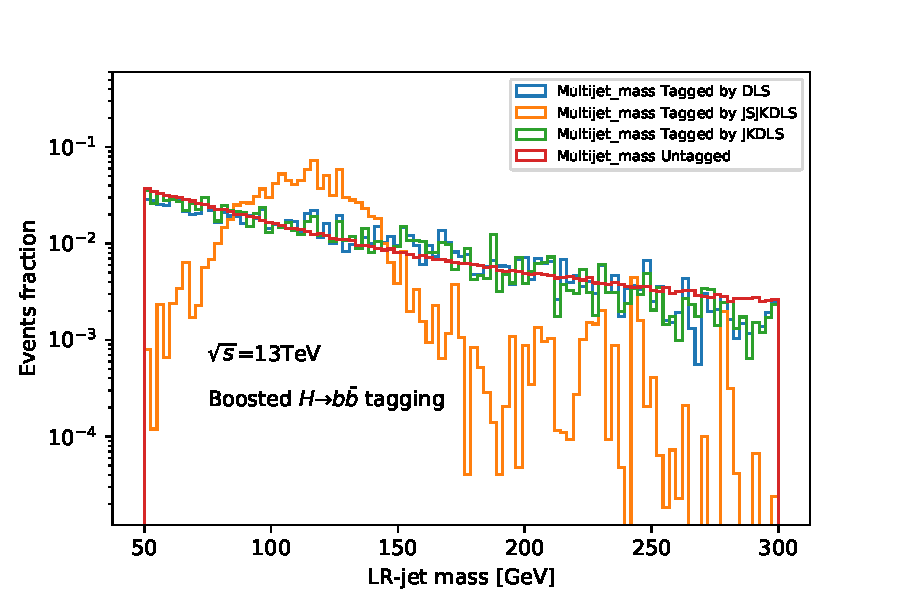
\includegraphics[width=0.75\textwidth]{figuresXbb/XbbTagger1.pdf}
  \end{center}
  \caption{
%基于变量控制的其中三个
模型DLS、JKDLS和JSJKDLS对multijet样本中LR-jet的质量分布的影响。
图中红线表示样本中LR-jet质量分布,
橘色、绿色和蓝色分别表示被模型JSJKDLS、JKDLS和DLS标定之后的LR-jet质量分布,
所有分布都已经归一化。
  }
    \label{fig:XbbTagger1}
\end{figure}


\subsection{优化器}
\label{sec:XbbTagger2}

%在
确定算法训练的输入变量
%集JK和DLS
之后,
接下来我们通过优化神经网络的结构参数来提高信号和本底的区分精度,
研究
%过程中
发现,
结构参数中优化器的选择对模型的性能有着比较显著的影响,这一小节将会介绍,
而其他结构参数对模型性能的影响非常小,将会在第~\ref{sec:XbbTagger4}~小节中介绍。

这里主要考虑了两种
%主流
常用的
的优化器\textsc{Adam}~\cite{Kingma:2014}和\textsc{SGD}~\cite{SGD}。
通过控制其他结构参数一致,对基于这两种优化器的模型进行了性能对比,
%通过仅控制神经网络中优化器不同,对训练出来的两个模型进行性能对比,
%如图~\ref{fig:XbbTagger2}~所示,
%展示的是以multijet作为本底时,两个模型的本底排除率随着信号效率的变化关系对比,
图~\ref{fig:XbbTagger2}~展示了两种模型的本底排除率随着信号效率的变化关系对比,
其中以multijet样本作为本底进行评估。
可以看到,使用优化器\textsc{Adam}可以显著提升模型的性能。
于是,我们将\textsc{Adam}作为最终用于算法训练的优化器。
%因此,我将\textsc{Adam}作为最终用于算法训练的优化器。

\begin{figure}
  \begin{center}
    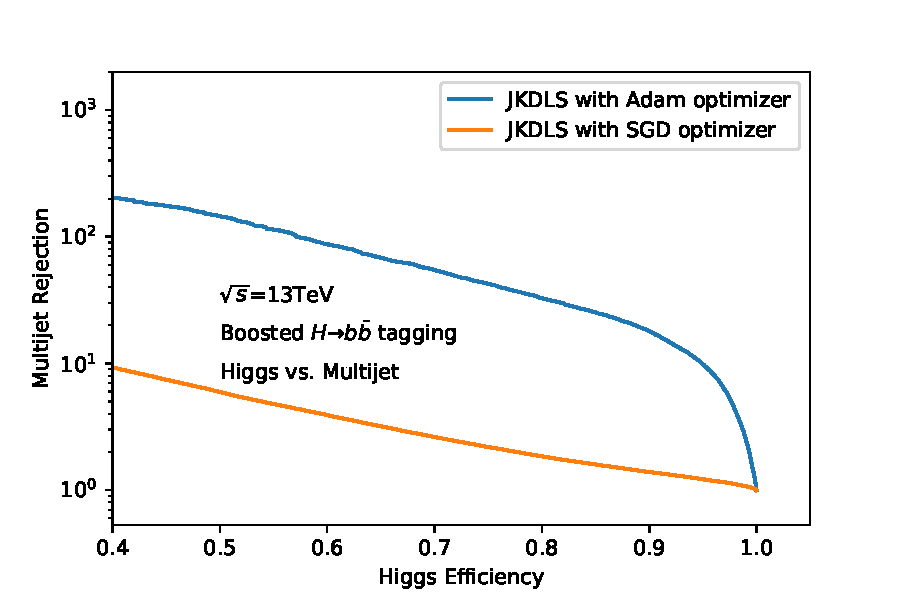
\includegraphics[width=0.75\textwidth]{figuresXbb/XbbTagger2a.pdf}
  \end{center}
  \caption{
  以multijet样本作为本底时,基于优化器\textsc{Adam}和\textsc{SGD}的两种模型的本底排除率随着信号效率的变化关系对比。
%选择不同的优化器\textsc{Adam}和\textsc{SGD}进行训练时,模型JKDLS的性能对比。
  }
    \label{fig:XbbTagger2}
\end{figure}


\subsection{输入subjet个数}
\label{sec:XbbTagger25}

为了说明算法训练的输入中包含领头LR-jet中的横动量最高的三个subjet的味标定信息相对于
仅包含两个subjet的信息,能为算法性能带来显著的提升,
%算法训练的输入中包含LR-jet中的横动量最高的两个subjet的味标定信息来说可以为算法性能带来显著的提升,
这里分别在这两种情况下进行训练,并对比了相应的模型性能,
并将这两个模型分别记为JKDLS(3-subjets)和JKDLS(2-subjets)。
%将使用LR-jet中的横动量最高的三个和两个subjet的味标定信息训练出来的模型分别记为JKDLS(3-subjets)和JKDLS(3-subjets)。

如图~\ref{fig:SUBLOSS}~所示,
在性能对比之前,
我们首先检查了两种模型中训练样本和验证样本的损失函数在训练过程中的变化趋势,
左图展示的是模型JKDLS(3-subjets)训练过程中损失函数随着训练时期(Epoch)的变化,
右图对应于模型JKDLS(2-subjets)。
%右图展示的是模型JKDLS(3-subjets)训练过程中损失函数随着训练时期的变化。
%图中训练在没到200个训练时期的时候就中断了是因为训练过程采用了EarlyStop~\cite{EarlyStop}的技术,
图中训练时期没有到达200是因为训练过程采用了EarlyStop~\cite{EarlyStop}的技术,
它是通过监督训练过程中验证样本的损失函数的变化来判断训练是否终止,
这种技术可以有效的防止过拟合,也可以节省时间。
%图中
可以看到两种模型中训练样本和验证样本的损失函数都是收敛的,
这表明训练过程都是可接受的,没有出现过拟合的现象。

\begin{figure}[htbp]
  \begin{subfigure}{.5\textwidth}
  \centering
   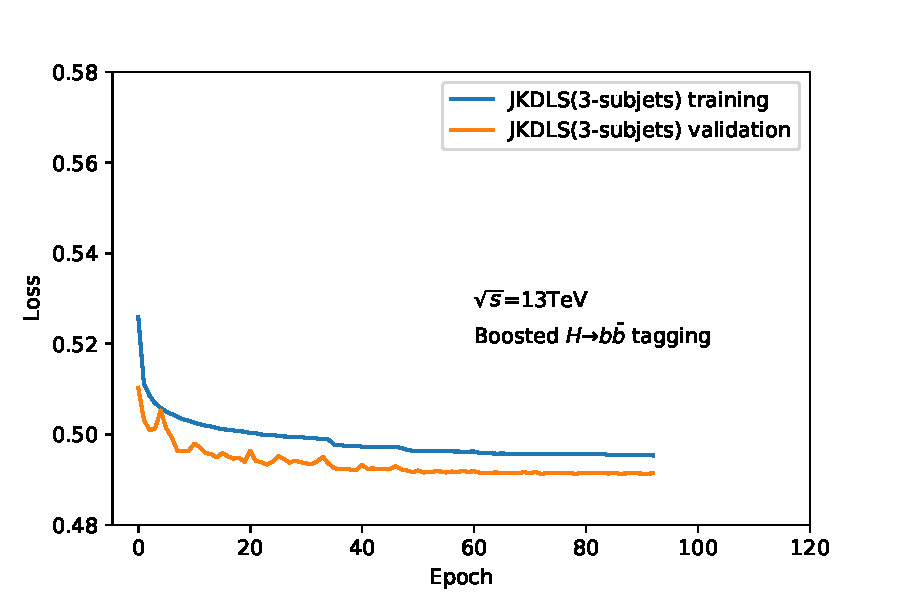
\includegraphics[width=0.99\textwidth]{figuresXbb/Subjet/SUB3Loss.pdf}
   \caption{JKDLS(3-subjets)}
   %\label{fig:}
  \end{subfigure}
  \begin{subfigure}{.5\textwidth}
  \centering
   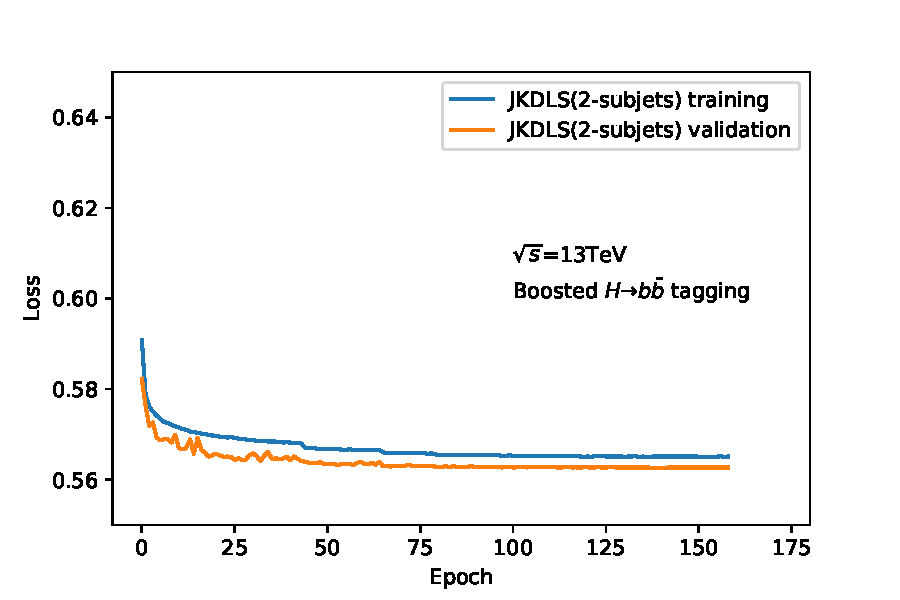
\includegraphics[width=0.99\textwidth]{figuresXbb/Subjet/SUB2Loss.pdf}
   \caption{JKDLS(2-subjets)}
   %\label{fig:}
  \end{subfigure}
  \caption{ 
模型JKDLS(3-subjets)和JKDLS(2-subjets)的训练样本和验证样本的损失函数在训练过程中
随着训练时期的变化。
左图对应于模型JKDLS(3-subjets),右图对应于模型JKDLS(2-subjets)。
%的变化趋势。
%左图展示的是模型JKDLS(3-subjets)训练过程中损失函数随着训练时期的变化,
%右图展示的是模型JKDLS(3-subjets)训练过程中损失函数随着训练时期的变化。
%图中训练在没到200个训练时期的时候就中断了是因为训练过程采用了EarlyStop~\cite{EarlyStop}的技术。
   }
  \label{fig:SUBLOSS}
\end{figure} 

接着对两种模型的性能进行了对比,
在multijet和t夸克两种本底的排除率与信号效率的变化关系的对比中,
选取了以下五个区间进行全方位的对比:
\begin{itemize}
       \item 仅包含第~\ref{sec:XbbOR}~小节中筛选条件的全包含区间,记为Inclusive。
       \item 除了第~\ref{sec:XbbOR}~小节描述的筛选条件之外,还要求事例中领头LR-jet的质量在76GeV和146GeV之间,即$m_{J}\in[76,146]GeV$, 
       在上一轮研究~\cite{TAGGING5}当中,在LR-jet横动量大于250GeV的情况下,这个质量区间所包含的Higgs-jet的数量占总数的90\%。
       \item 除了第~\ref{sec:XbbOR}~小节描述的筛选条件和$m_{J}\in [76,146]GeV$,还要求事例中领头LR-jet的横动量在250GeV和500GeV之间,
       即低横动量区间$p_{T}^{J}\in [250,500]GeV$。
       \item 除了第~\ref{sec:XbbOR}~小节描述的筛选条件和$m_{J}\in [76,146]GeV$,还要求事例中领头LR-jet的横动量在500GeV和1000GeV之间,
       即中横动量区间$p_{T}^{J}\in [500,1000]GeV$。
       \item 除了第~\ref{sec:XbbOR}~小节描述的筛选条件和$m_{J}\in [76,146]GeV$,还要求事例中领头LR-jet的横动量在1000GeV和3000GeV之间,
       即高横动量区间$p_{T}^{J}\in [1000,3000]GeV$。
\end{itemize}
如图~\ref{fig:SubjetROC}~所示,
对于
%两种
模型JKDLS(3-subjets)和JKDLS(2-subjets),
左排的图展示的是multijet本底排除率随着信号效率的变化关系的对比,
右排的图展示的是t夸克本底排除率随着信号效率的变化关系的对比,
从上到下依次对应于五个区间
Inclusive、$m_{J}\in [76,146]GeV$、
$m_{J}\in [76,146]GeV, p_{T}^{J}\in [250,500]GeV$、
$m_{J}\in [76,146]GeV, p_{T}^{J}\in [500,1000]GeV$、
$m_{J}\in [76,146]GeV, p_{T}^{J}\in [1000,3000]GeV$,
%的性能对比,
图中
还展示了
%下半部分是
在信号效率相同时,两种模型对应的本底排除率的比值。
可以看到模型JKDLS(3-subjets)相对于模型JKDLS(2-subjets)的性能提升非常明显,
尤其是在t夸克本底的排除率与信号效率的变化关系的对比中,
在高横动量区间更为显著,在信号效率为60\%的情况下,
模型JKDLS(3-subjets)的t夸克本底排除率大约为模型JKDLS(2-subjets)的1.8倍。
这主要
%是
依赖于t夸克的性质~\cite{PDG},
t夸克主要的衰变模式是$t\to b+W^+, \bar{t}\to \bar{b}+W^-$,
而强子型衰变的t夸克产生的W玻色子随后衰变成两个夸克,
即t夸克样本中,LR-jet包含三个subjet的事例占主导,
%即t夸克样本中事例以LR-jet中包含3个subjet为主导,
因此模型JKDLS(3-subjets)的性能更优。


\begin{figure}[htbp]
  \begin{subfigure}{.5\textwidth}
  \centering
   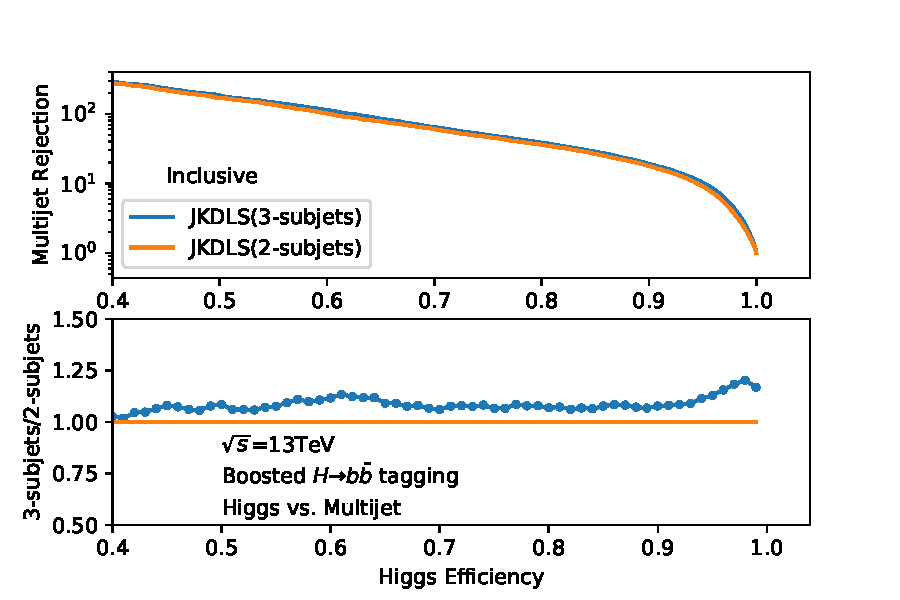
\includegraphics[width=0.75\textwidth]{figuresXbb/Subjet/SUBQCD.pdf}
   %\caption{Higgs vs. Multijet, inclusive}
   \caption{}
   %\label{fig:}
  \end{subfigure}
  \begin{subfigure}{.5\textwidth}
  \centering
   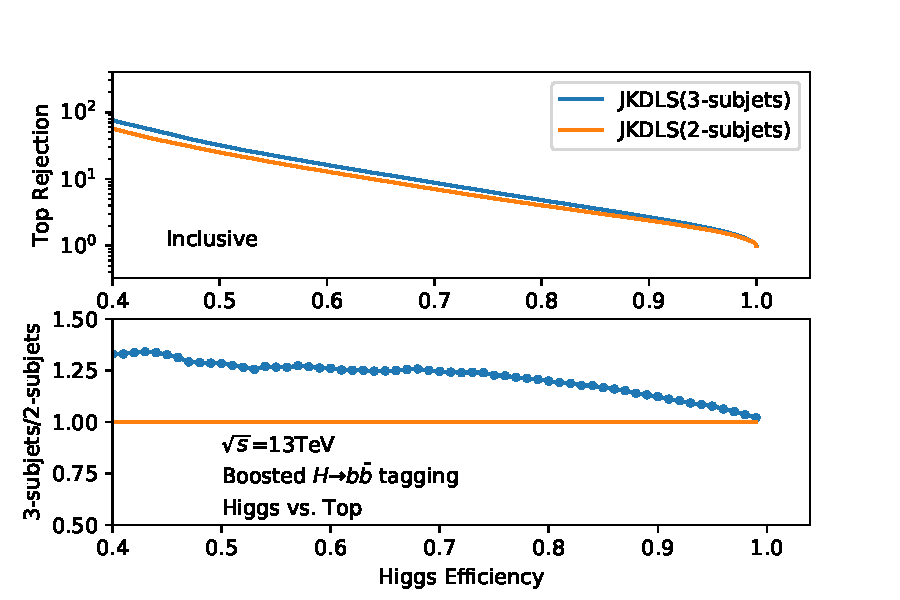
\includegraphics[width=0.75\textwidth]{figuresXbb/Subjet/SUBTop.pdf}
   %\caption{Higgs vs. Top, Inclusive}
     \caption{}
   %\label{fig:}
  \end{subfigure}
\newline 
   \begin{subfigure}{.5\textwidth}
  \centering
   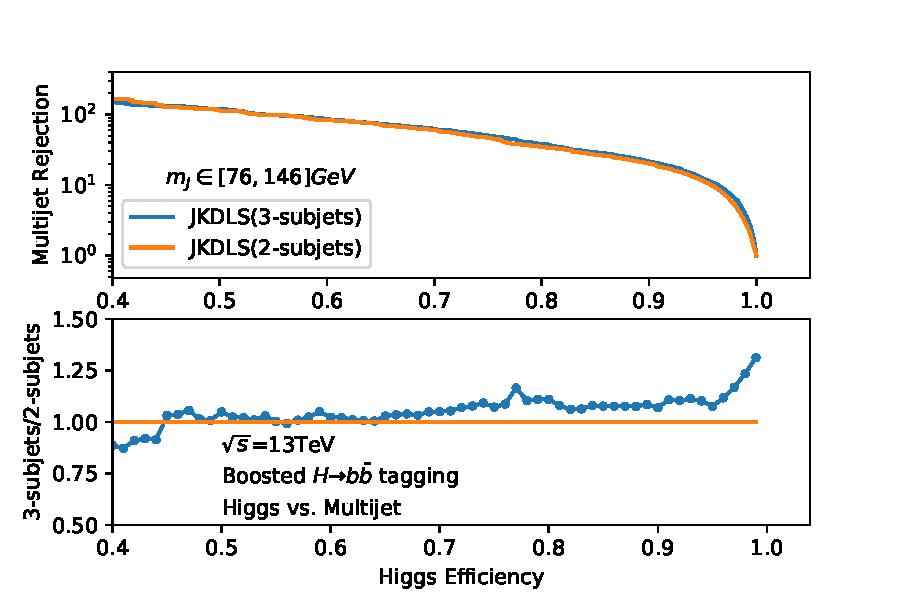
\includegraphics[width=0.75\textwidth]{figuresXbb/Subjet/SUBQCDMASS.pdf}
   %\caption{Higgs vs. Multijet, $m_{J}\in [76,146]GeV$}
     \caption{}
   %\label{fig:}
  \end{subfigure}
  \begin{subfigure}{.5\textwidth}
  \centering
   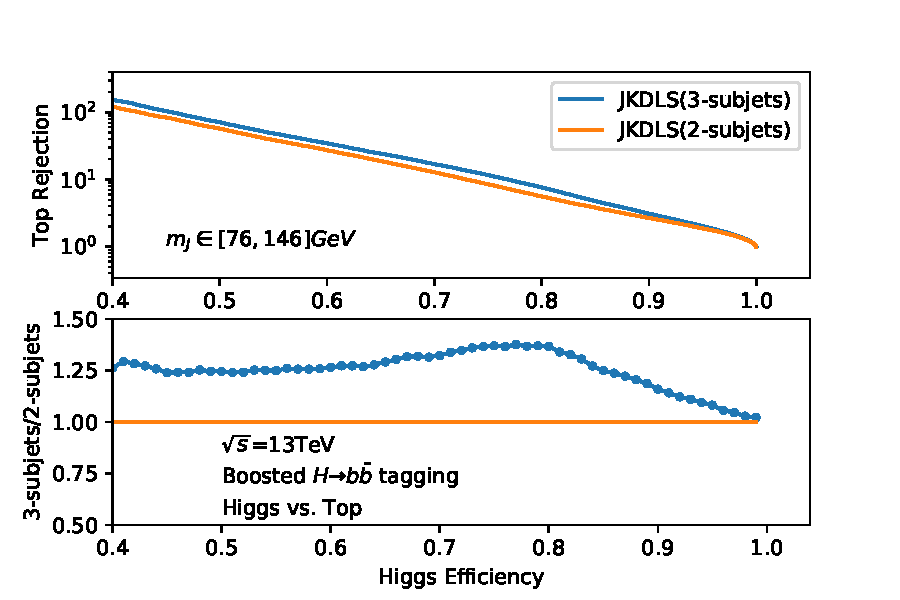
\includegraphics[width=0.75\textwidth]{figuresXbb/Subjet/SUBTopMASS.pdf}
   %\caption{Higgs vs. Top, $m_{J}\in [76,146]GeV$}
     \caption{}
   %\label{fig:}
  \end{subfigure}
 \newline 
   \begin{subfigure}{.5\textwidth}
  \centering
   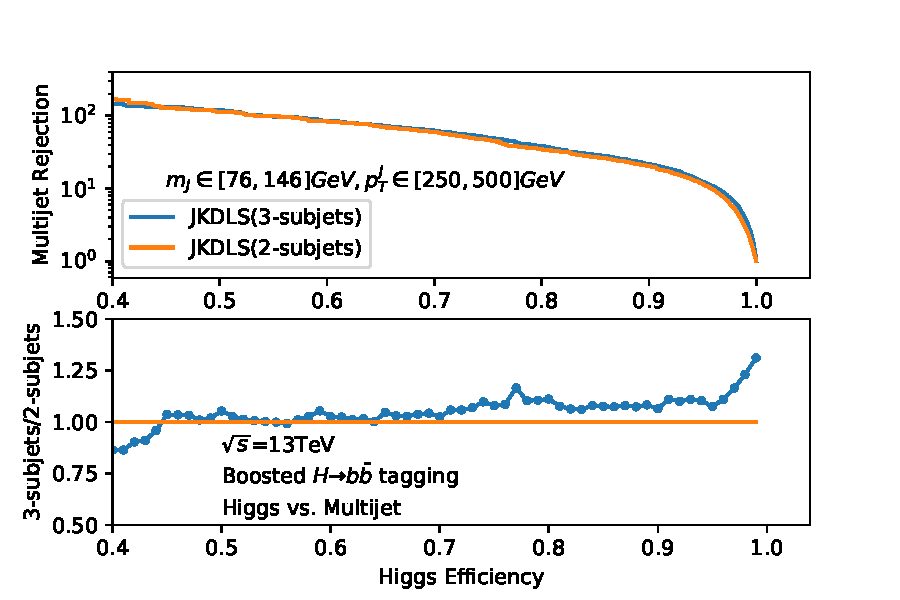
\includegraphics[width=0.75\textwidth]{figuresXbb/Subjet/SUBQCDMASSPT1.pdf}
   %\caption{Higgs vs. Multijet, $m_{J}\in [76,146]GeV, p_{T}^{J}\in [250,500]GeV$}
     \caption{}
   %\label{fig:}
  \end{subfigure}
  \begin{subfigure}{.5\textwidth}
  \centering
   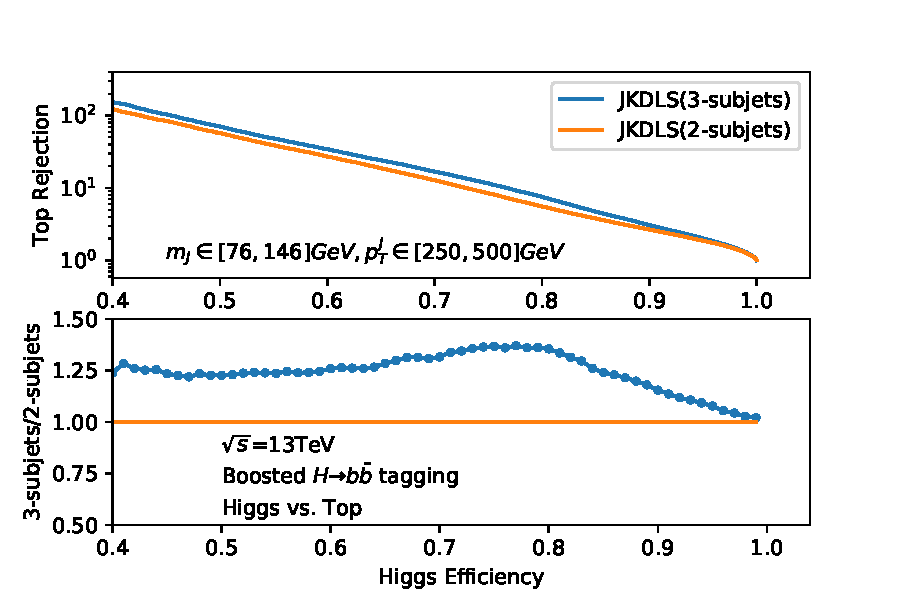
\includegraphics[width=0.75\textwidth]{figuresXbb/Subjet/SUBTopMASSPT1.pdf}
   %\caption{Higgs vs. Top, $m_{J}\in [76,146]GeV, p_{T}^{J}\in [250,500]GeV$}
     \caption{}
   %\label{fig:}
  \end{subfigure}
 \newline 
   \begin{subfigure}{.5\textwidth}
  \centering
   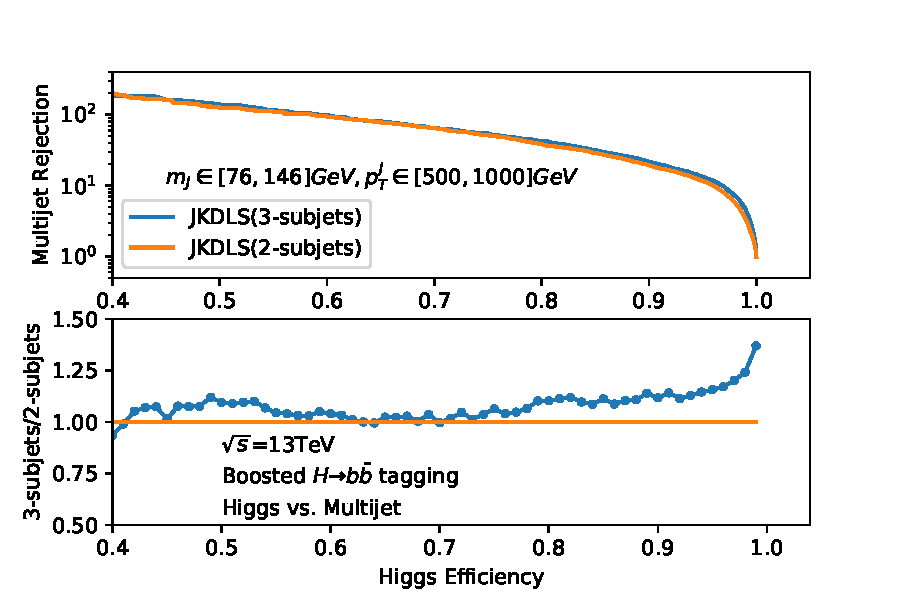
\includegraphics[width=0.75\textwidth]{figuresXbb/Subjet/SUBQCDMASSPT2.pdf}
   %\caption{Higgs vs. Multijet, $m_{J}\in [76,146]GeV, p_{T}^{J}\in [500,1000]GeV$}
     \caption{}
   %\label{fig:}
  \end{subfigure}
  \begin{subfigure}{.5\textwidth}
  \centering
   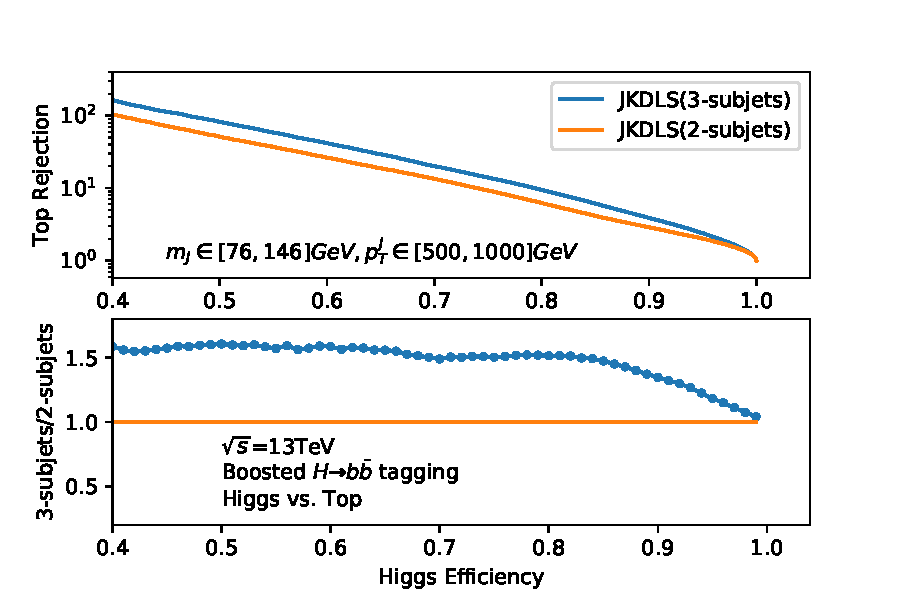
\includegraphics[width=0.75\textwidth]{figuresXbb/Subjet/SUBTopMASSPT2.pdf}
   %\caption{Higgs vs. Top, $m_{J}\in [76,146]GeV, p_{T}^{J}\in [500,1000]GeV$}
     \caption{}
   %\label{fig:}
  \end{subfigure}
 \newline 
   \begin{subfigure}{.5\textwidth}
  \centering
   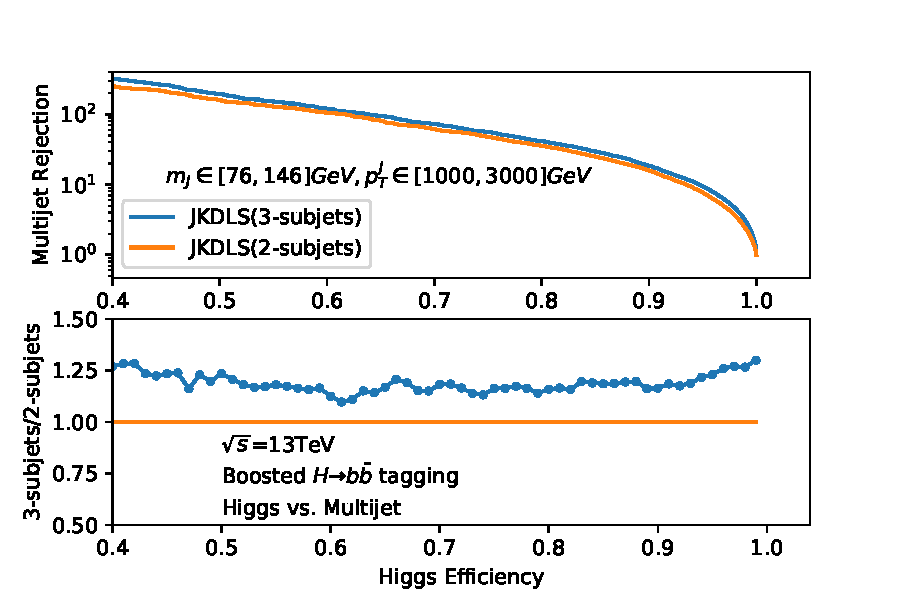
\includegraphics[width=0.75\textwidth]{figuresXbb/Subjet/SUBQCDMASSPT3.pdf}
   %\caption{Higgs vs. Multijet, $m_{J}\in [76,146]GeV, p_{T}^{J}\in [1000,3000]GeV$}
     \caption{}
   %\label{fig:}
  \end{subfigure}
  \begin{subfigure}{.5\textwidth}
  \centering
   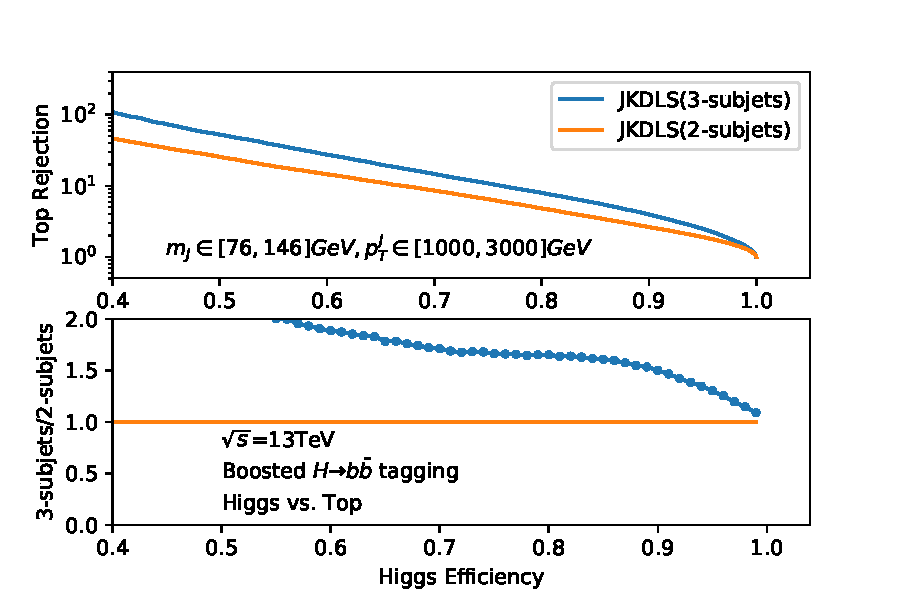
\includegraphics[width=0.75\textwidth]{figuresXbb/Subjet/SUBTopMASSPT3.pdf}
   %\caption{Higgs vs. Top, $m_{J}\in [76,146]GeV, p_{T}^{J}\in [1000,3000]GeV$}
     \caption{}
   %\label{fig:}
  \end{subfigure}
  \caption{
 模型JKDLS(3-subjets)和JKDLS(2-subjets)的性能对比。
左排的图展示的是multijet本底排除率随着信号效率的变化关系的对比,
右排的图展示的是t夸克本底排除率随着信号效率的变化关系的对比,
从上到下依次对应于第~\ref{sec:XbbTagger25}~小节中定义的五个区间。
%的性能对比。
  }
  \label{fig:SubjetROC}
\end{figure} 


\subsection{加权策略}
\label{sec:XbbTagger3}

接下来,通过在训练时引入不同的加权策略,
我们比较了两种加权方式对
模型性能的影响。
%训练出来的模型的影响。
第一种称为分布采样(Resampling),
在不给样本中事例赋予权重的情况下,
同时对
%信号和本底共
三个样本进行采样,
使得领头LR-jet的横动量分布中每个bin的事例数等于三个样本中最小的事例数,
如图~\ref{fig:ReweightPt}~中左图所示,
分布采样的结果是三个样本中领头LR-jet的横动量分布都是相同的,
随后,同样在不赋予权重的情况下
%对算法
进行训练。
第二种称为分布加权(Reweighting),给信号样本和t夸克样本中每个事例重新赋予权重,
如图~\ref{fig:ReweightPt}~中右图所示,
在包含事例权重的情况下,
分布加权的结果是信号样本和t夸克样本中领头LR-jet的横动量分布与multijet样本中领头LR-jet的横动量分布是一致的。
随后,在包含事例权重的情况下
%对算法
进行训练。
这两种加权方式都能防止
%训练出来的
模型在训练时学会识别
%三个
样本中LR-jet
%不同
的运动学特性。

\begin{figure}[htbp]
  \begin{subfigure}{.5\textwidth}
  \centering
   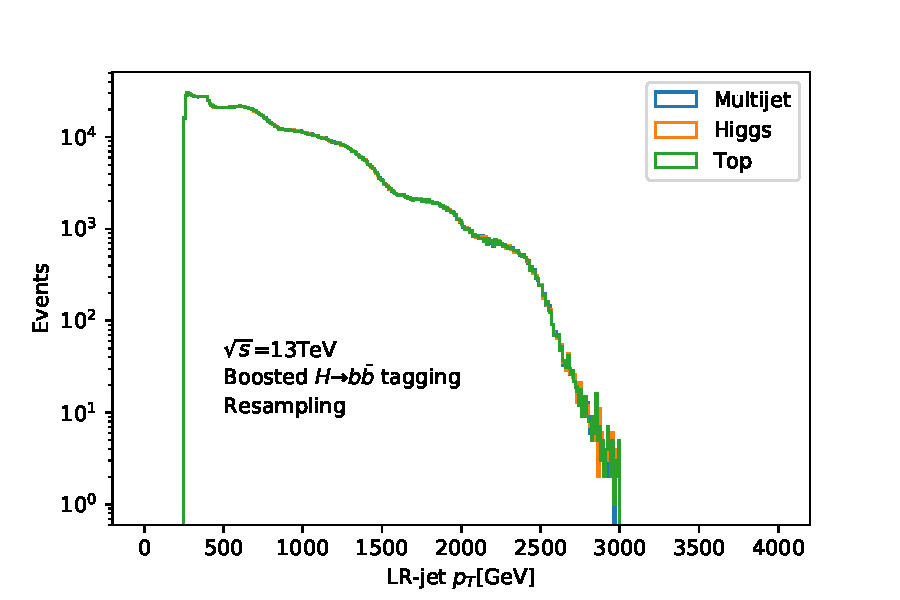
\includegraphics[width=0.99\textwidth]{figuresXbb/resample.pdf}
   \caption{Resampling}
   \label{fig:resample}
  \end{subfigure}
  \begin{subfigure}{.5\textwidth}
  \centering
   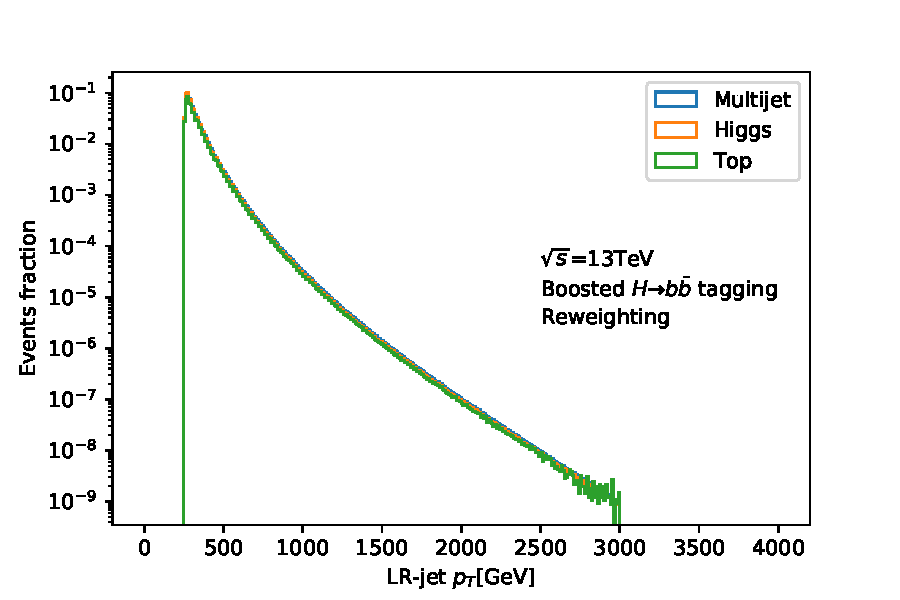
\includegraphics[width=0.99\textwidth]{figuresXbb/reweight.pdf}
   \caption{Reweighting}
   \label{fig:reweight}
  \end{subfigure}
  \caption{
  %算法训练过程中,
  两种不同的加权策略。左图表示分布采样,右图表示分布加权。
  }
  \label{fig:ReweightPt}
\end{figure} 

如图~\ref{fig:WEILOSS}~所示,
同样,
我们先检查了上述两种模型中训练样本和验证样本的损失函数在训练过程中随着训练时期的变化。
左图对应于基于分布采样的模型,
右图对应于基于分布加权的模型。
%的变化趋势,
%左图展示的是基于分布采样训练出来的模型在训练过程中损失函数随着训练时期的变化,
%右图展示的是基于分布加权训练出来的模型在训练过程中损失函数随着训练时期的变化。
%图中训练在没到200个训练时期的时候就中断了是因为训练过程采用了EarlyStop的技术。
图中训练时期没有到达200是因为训练过程采用了EarlyStop的技术。
%图中
可以看到训练样本和验证样本的损失函数都是收敛的,
这表明
%训练过程都是可接受的,
没有出现过拟合的现象。

\begin{figure}[htbp]
  \begin{subfigure}{.5\textwidth}
  \centering
   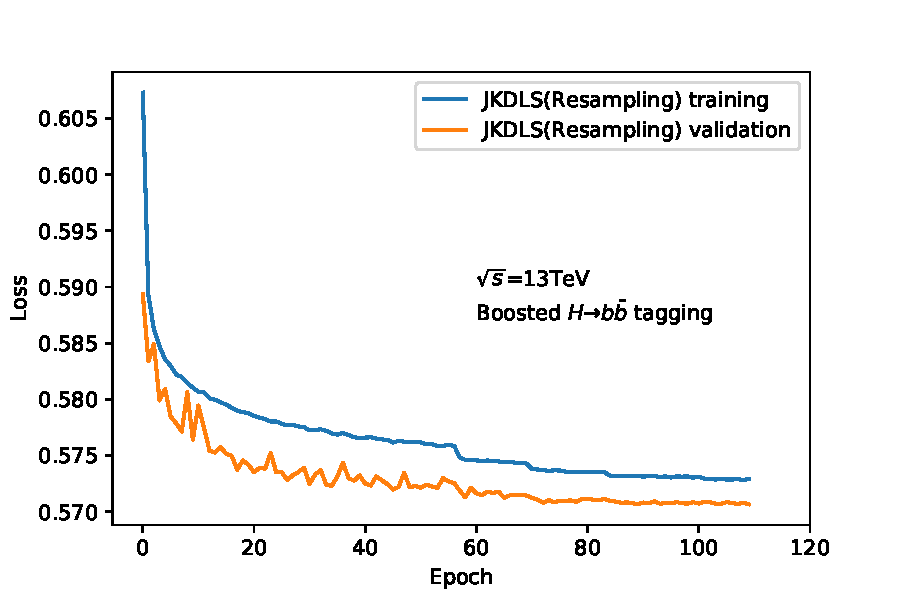
\includegraphics[width=0.99\textwidth]{figuresXbb/Reweight/LOSSResample.pdf}
   \caption{JKDLS using resampling strategy}
   %\label{fig:}
  \end{subfigure}
  \begin{subfigure}{.5\textwidth}
  \centering
   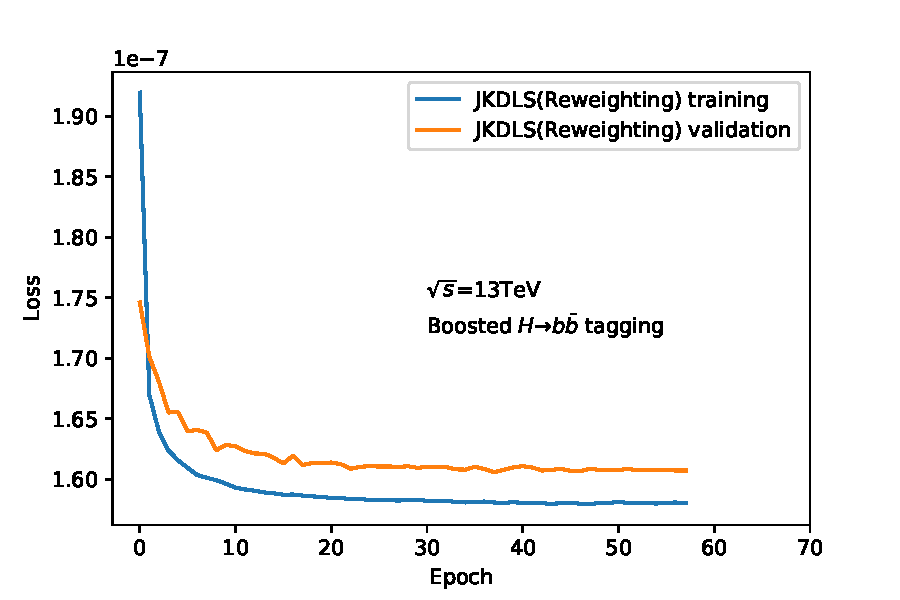
\includegraphics[width=0.99\textwidth]{figuresXbb/Reweight/LOSSReweight.pdf}
   \caption{JKDLS using reweighting strategy}
   %\label{fig:}
  \end{subfigure}
  \caption{ 
 基于分布采样(左图)和分布加权(右图)的模型中训练样本和验证样本的损失函数在训练过程中随着训练时期的变化。
%左图对应于基于分布采样的模型,
%右图对应于基于分布加权的模型。
 % 基于两种加权方式训练出来的模型的训练样本和验证样本的损失函数在训练过程中的变化趋势。
%左图展示的是基于分布采样训练出来的模型在训练过程中损失函数随着训练时期的变化,
%右图展示的是基于分布加权训练出来的模型在训练过程中损失函数随着训练时期的变化。
%图中训练在没到200个训练时期的时候就中断了是因为训练过程采用了EarlyStop的技术。
   }
  \label{fig:WEILOSS}
\end{figure} 



接着对比了上述
两种模型的性能,
%两个加权方式训练出来的模型性能,
如图~\ref{fig:ReweightROC}~所示,
左排的图展示的是
%模型的
multijet本底排除率随着信号效率的变化关系对比,
右排的图展示的是
%模型的
t夸克本底排除率随着信号效率的变化关系对比,
从上到下依次对应于第~\ref{sec:XbbTagger25}~小节中定义的五个区间。
%的性能对比,
%图中下半部分是在信号效率相同时,两种模型对应的本底排除率的比值。
从图中可以看出基于分布采样
%训练出来
的模型的性能更优,
尤其是在高横动量区间,
在信号效率为60\%的情况下,基于分布采样
%训练出来
的模型的本底排除率大约为基于分布加权的模型的2倍。
于是,
在最终训练中,我们采用的分布采样的加权策略。
%我将分布采样作为最终用于算法训练的加权方式。

\begin{figure}[htbp]
  \begin{subfigure}{.5\textwidth}
  \centering
   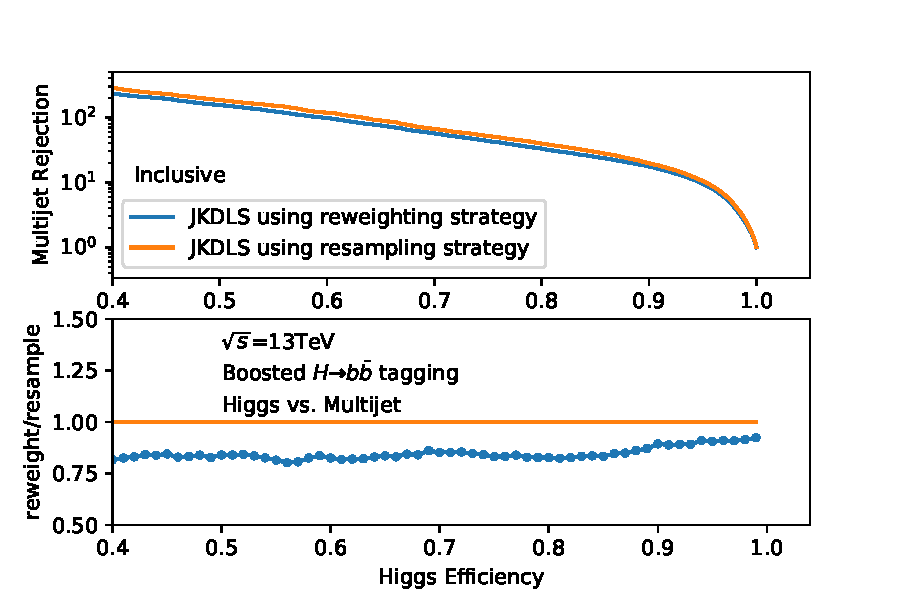
\includegraphics[width=0.75\textwidth]{figuresXbb/Reweight/QCDIN.pdf}
   \caption{}
   %\label{fig:}
  \end{subfigure}
  \begin{subfigure}{.5\textwidth}
  \centering
   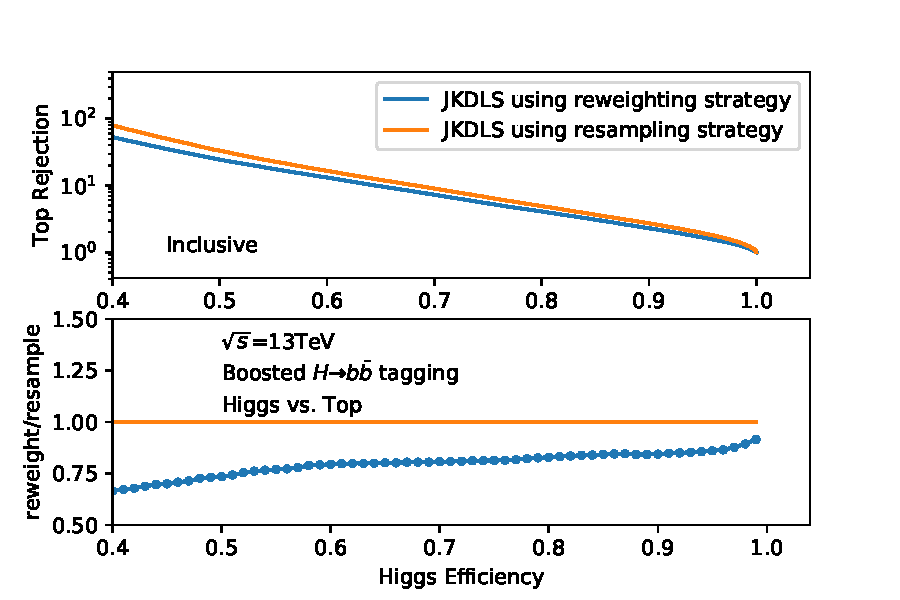
\includegraphics[width=0.75\textwidth]{figuresXbb/Reweight/TOPIN.pdf}
   \caption{}
   %\label{fig:}
  \end{subfigure}
\newline 
   \begin{subfigure}{.5\textwidth}
  \centering
   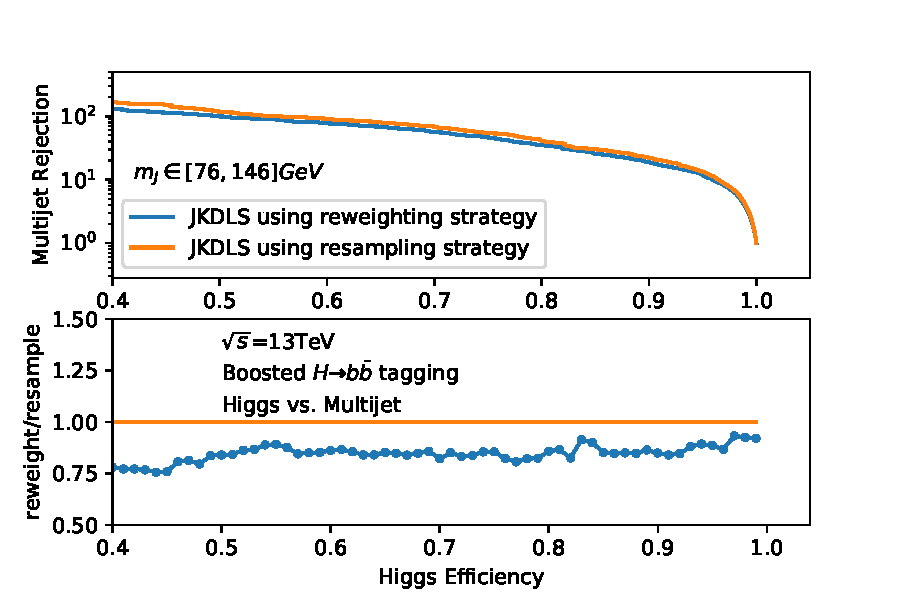
\includegraphics[width=0.75\textwidth]{figuresXbb/Reweight/QCDMASS.pdf}
   \caption{}
   %\label{fig:}
  \end{subfigure}
  \begin{subfigure}{.5\textwidth}
  \centering
   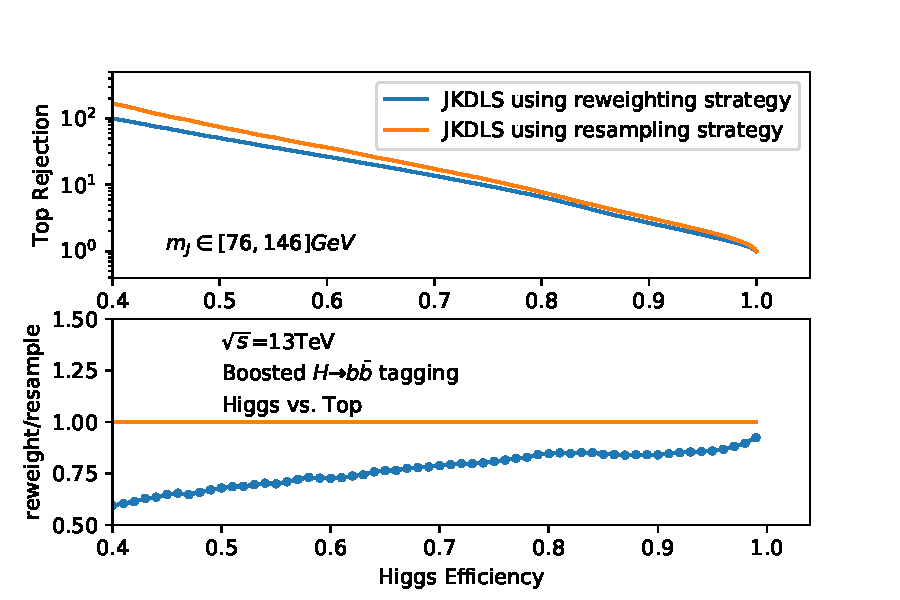
\includegraphics[width=0.75\textwidth]{figuresXbb/Reweight/TOPMASS.pdf}
   \caption{}
   %\label{fig:}
  \end{subfigure}
 \newline 
   \begin{subfigure}{.5\textwidth}
  \centering
   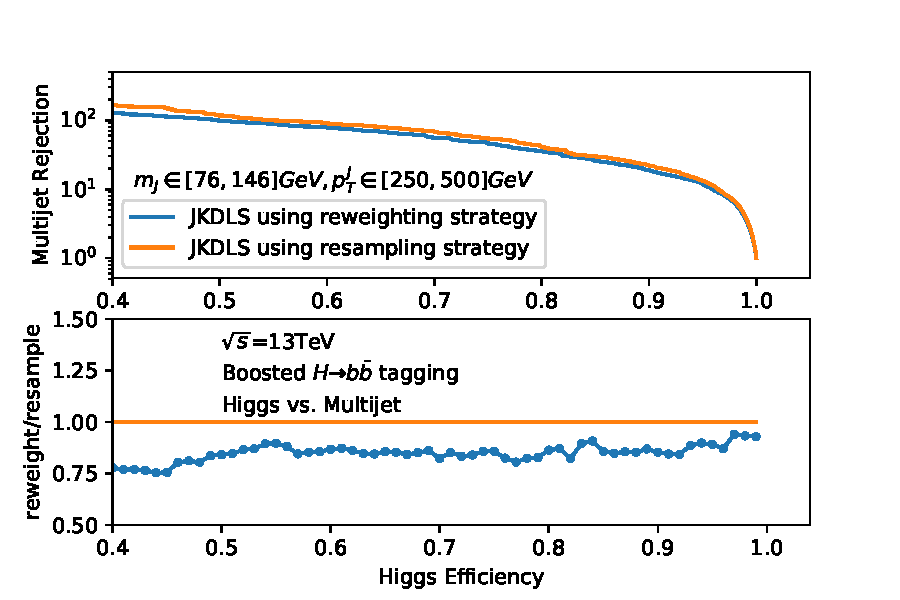
\includegraphics[width=0.75\textwidth]{figuresXbb/Reweight/QCDMASSPT1.pdf}
   \caption{}
   %\label{fig:}
  \end{subfigure}
  \begin{subfigure}{.5\textwidth}
  \centering
   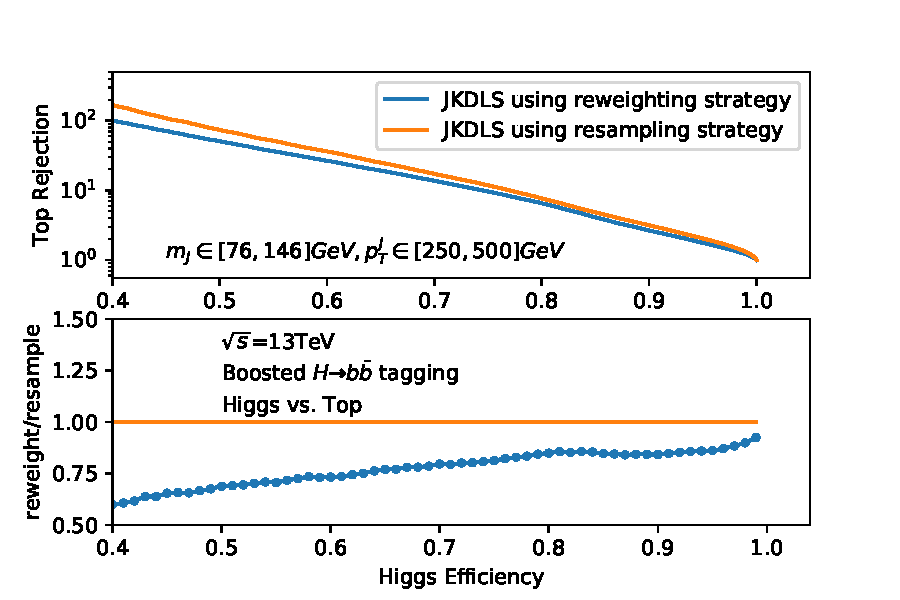
\includegraphics[width=0.75\textwidth]{figuresXbb/Reweight/TOPMASSPT1.pdf}
   \caption{}
   %\label{fig:}
  \end{subfigure}
 \newline 
   \begin{subfigure}{.5\textwidth}
  \centering
   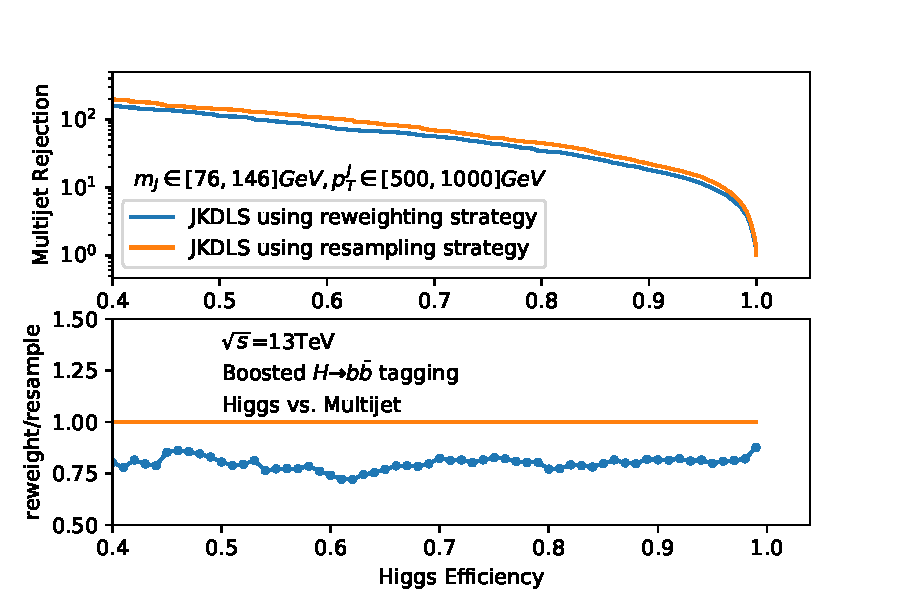
\includegraphics[width=0.75\textwidth]{figuresXbb/Reweight/QCDMASSPT2.pdf}
   \caption{}
   %\label{fig:}
  \end{subfigure}
  \begin{subfigure}{.5\textwidth}
  \centering
   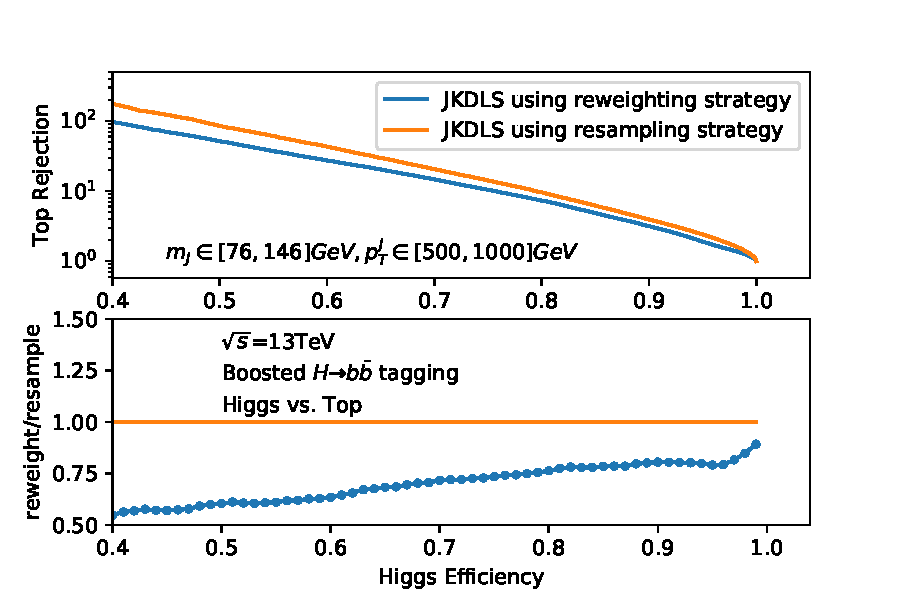
\includegraphics[width=0.75\textwidth]{figuresXbb/Reweight/TOPMASSPT2.pdf}
   \caption{}
   %\label{fig:}
  \end{subfigure}
 \newline 
   \begin{subfigure}{.5\textwidth}
  \centering
   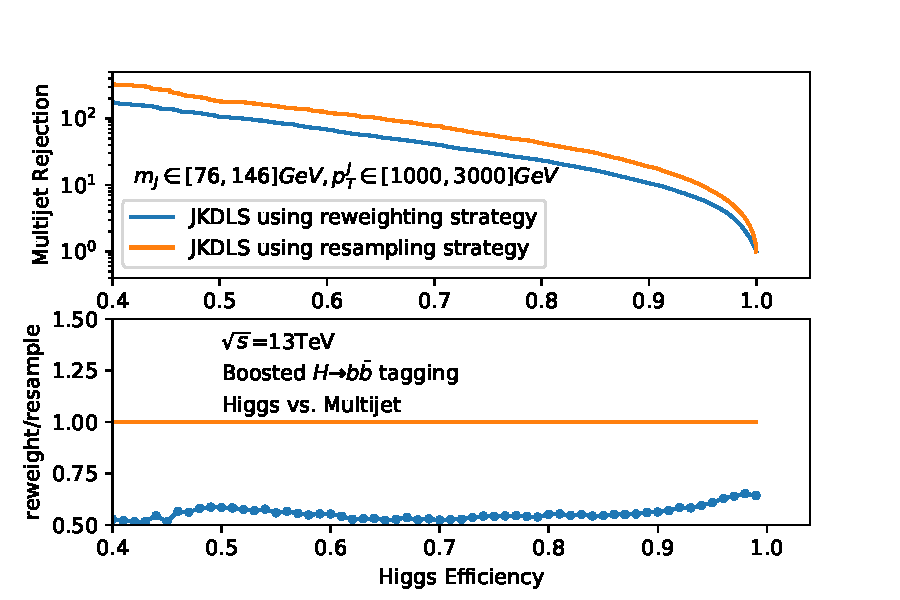
\includegraphics[width=0.75\textwidth]{figuresXbb/Reweight/QCDMASSPT3.pdf}
   \caption{}
   %\label{fig:}
  \end{subfigure}
  \begin{subfigure}{.5\textwidth}
  \centering
   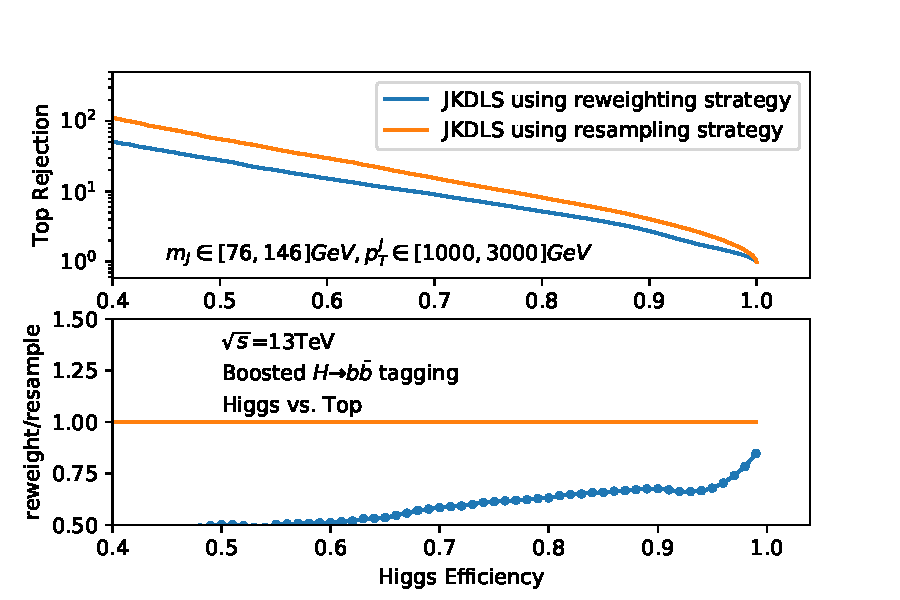
\includegraphics[width=0.75\textwidth]{figuresXbb/Reweight/TOPMASSPT3.pdf}
   \caption{}
   %\label{fig:}
  \end{subfigure}
  \caption{
  基于分布采样和分布加权的模型的性能对比。
  左排的图展示的是multijet本底排除率随着信号效率的变化关系对比,
右排的图展示的是t夸克本底排除率随着信号效率的变化关系对比,
从上到下依次对应于第~\ref{sec:XbbTagger25}~小节中定义的五个区间。
  %选择不同的加权方式进行训练时,模型JKDLS的性能对比。
 % 左边的图展示的是模型的multijet本底排除率与信号效率的变化关系的对比,
%右边的图展示的是模型的t夸克本底排除率与信号效率的变化关系的对比,
%从上到下依次对应于五个区间的性能对比。
  }
  \label{fig:ReweightROC}
\end{figure} 




\subsection{结构参数优化}
\label{sec:XbbTagger4}

在输入变量、优化器和加权策略得到优化
%并选定
之后,
我们
%随后
利用\textsc{Talos}~\cite{TALOS}对神经网络的其他结构参数进行了优化。
首先,
将表~\ref{tab:Hyper}~中的结构参数
%的神经网络
作为对照组(Monitored),
%选取了具有表~\ref{tab:Hyper}~中结构的神经网络作为对照组(Monitored),
这也是前四个小节的研究所使用的结构参数。
%算法的输出有$p_{\text{Higgs}}$、$p_{\text{multijet}}$和$p_{\text{top}}$三个,
%分别代表LR-jet被标定为Higgs-jet、QCD-jet和Top-jet的概率。
%用于训练、验证和测试的样本是分开的,其中用于训练的样本容量有$6\times 10^{6}$。

\begin{table}[ht]
\caption{用于对照组算法训练的神经网络的结构参数。}
\begin{center}
%\begin{adjustbox}{width=\columnwidth,center}
\begin{tabular}{c|c}
    \hline
    \hline
    Parameter & Value or type  \\
    \hline  
    Loss & Categorical crossentropy \\
    \hline  
    Hidden layers & 6 \\
    \hline  
    Nodes per hidden layers & 250 \\
    \hline  
    Learning rate & $10^{-2}$\\
    \hline  
    Learning rate decay & $10^{-5}$ \\
    \hline  
    Activation of inner layers & \textsc{ReLU}~\cite{Glorot:2011} \\
    \hline  
    Activation of outer layers & \textsc{SoftMax}~\cite{MLMIT} \\
    \hline  
    Batch normalization~\cite{Ioffe:2015} & $10^{4}$ \\
    \hline  
    Epoch & 200 \\
    \hline
    \hline
\end{tabular}
%\end{adjustbox}
\end{center}
\label{tab:Hyper}
\end{table}

在
%结构参数的
优化过程中,
我们扫描了
%如
表~\ref{tab:Space}~
中
%所示的
分立的参数空间,
总共有108个实验。
%然后比较这108个实验的训练结果,
在训练的过程中,验证样本的损失函数的变化对于训练好坏的判定来说更具有参考价值,
因此我们选取了验证样本的损失函数最小的那组结构作为优化后的结构参数,称为优化组(Optimized),
并对比了对照组模型和优化组模型的性能。

\begin{table}[ht]
\caption{用于算法训练的神经网络结构参数优化的参数空间。}
\begin{center}
%\begin{adjustbox}{width=\columnwidth,center}
\begin{tabular}{c|c}
    \hline
    \hline
    Parameter & Search space  \\
    \hline  
    Hidden layers & [4,6,8] \\
    \hline  
    Nodes per hidden layers & [50,120,250,500] \\
    \hline  
    Learning rate & [$10^{-1}$,$10^{-2}$,$10^{-3}$]\\
    \hline  
    Learning rate decay & [$10^{-3}$,$10^{-4}$,$10^{-5}$] \\
    \hline
    \hline
\end{tabular}
%\end{adjustbox}
\end{center}
\label{tab:Space}
\end{table}

结果表明,
优化组与对照组的结构参数相比,仅隐层
%(Hidden layers)
数目和学习速率
%(Learning rate)
不同,
对于优化组,它们分别为4层和$10^{-1}$。

在性能对比前,如图~\ref{fig:LOSS}~所示,
首先检查了对照组和优化组中训练样本和验证样本的损失函数在训练过程中随着训练时期的变化。
左图对应于对照组,右图对应于优化组。
%的变化趋势,
%左图展示的是基于分布采样训练出来的模型在训练过程中损失函数随着训练时期的变化,
%右图展示的是基于分布加权训练出来的模型在训练过程中损失函数随着训练时期的变化。
%图中训练在没到200个训练时期的时候就中断了是因为训练过程采用了EarlyStop的技术。
%图中训练时期没有到达200是因为训练过程采用了EarlyStop的技术。
可以看到训练样本和验证样本的损失函数都是收敛的,
这表明没有出现过拟合的现象。
%首先检查了对照组和优化组中训练样本和验证样本的损失函数在训练过程中的变化,
%左图展示的是对照组中损失函数随着训练时期的变化,
%右图展示的是优化组中损失函数随着训练时期的变化,
%可以在看到两组模型的训练中,用于训练和验证的损失函数都是收敛的,
%这表明训练过程都是可接受的,没有出现过拟合的现象。

\begin{figure}[htbp]
  \begin{subfigure}{.5\textwidth}
  \centering
   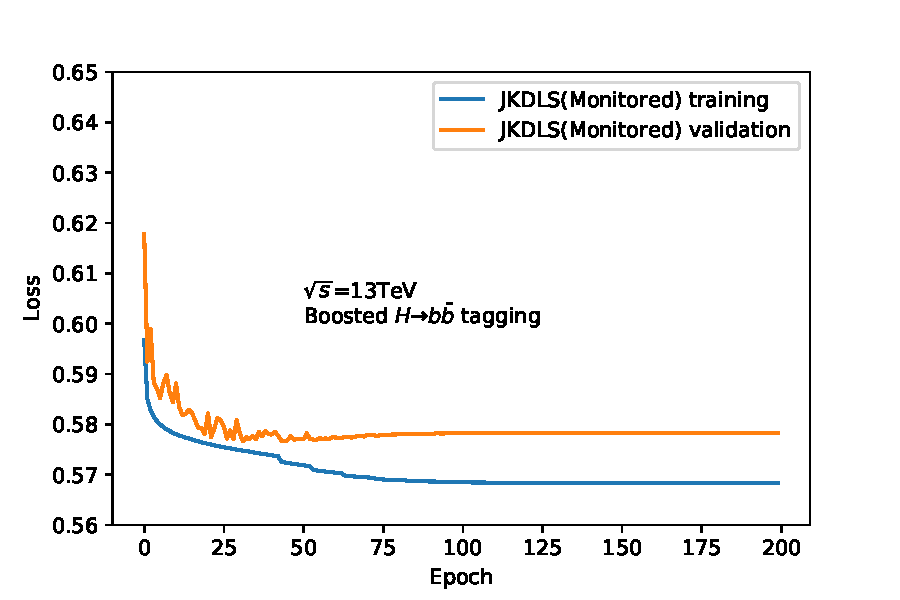
\includegraphics[width=0.99\textwidth]{figuresXbb/LossMON.pdf}
   \caption{Monitored}
   %\label{fig:}
  \end{subfigure}
  \begin{subfigure}{.5\textwidth}
  \centering
   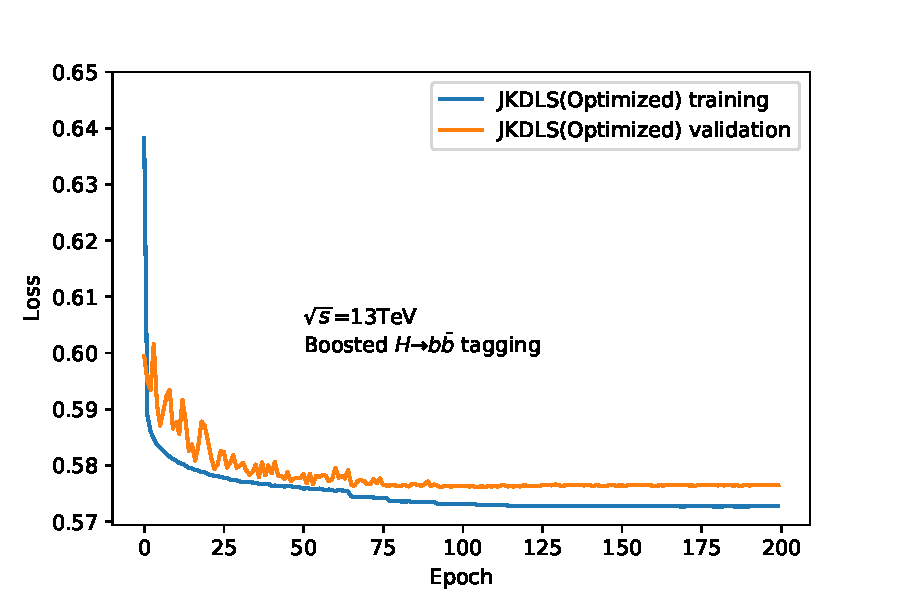
\includegraphics[width=0.99\textwidth]{figuresXbb/LossOPT.pdf}
   \caption{Optimized}
   %\label{fig:}
  \end{subfigure}
  \caption{
 对照组(左图)和优化组(右图)中训练样本和验证样本的损失函数在训练过程中随着训练时期的变化。
 左图对应于对照组,右图对应于优化组。
  }
  \label{fig:LOSS}
\end{figure} 

如图~\ref{fig:LOSSC}~所示,
随后我们对比了对照组和优化组中验证样本的损失函数在训练过程中的变化,
可以看到两组模型中
%用于验证
验证样本
的损失函数非常的接近,
这表明对照组的训练已经接近饱和,结构参数的优化对模型性能可能没有显著的提升。

\begin{figure}
  \begin{center}
    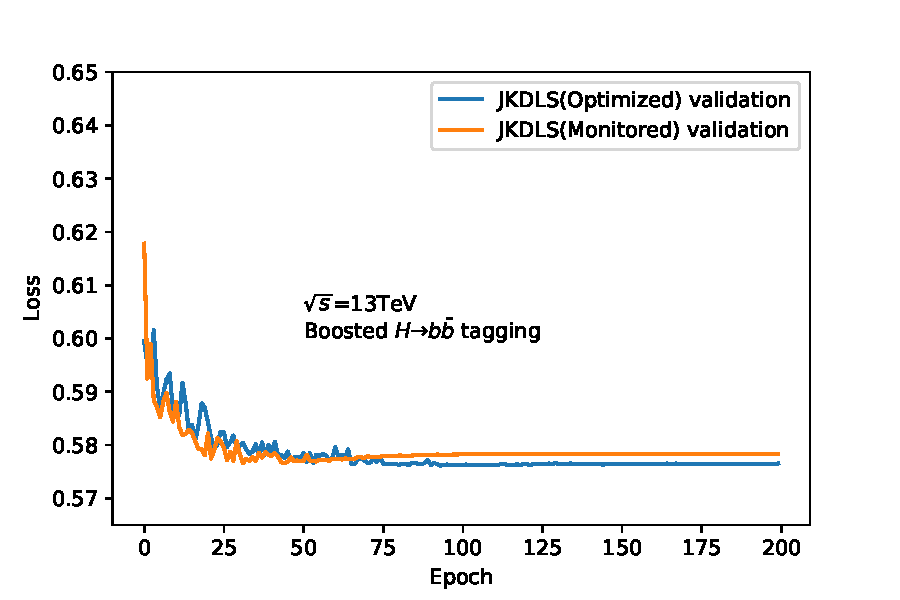
\includegraphics[width=0.75\textwidth]{figuresXbb/LossCOM.pdf}
  \end{center}
  \caption{
对照组和优化组中验证样本的损失函数在训练过程中随着训练时期的变化关系对比。
  }
    \label{fig:LOSSC}
\end{figure}

接下来,为了证实这一推断,
我们比较了两组模型的性能,
如图~\ref{fig:OPTROC}~所示,
对于对照组和优化组的模型,
左排的图展示的是multijet本底排除率随着信号效率的变化关系对比,
右排的图展示的是t夸克本底排除率随着信号效率的变化关系对比,
从上到下依次对应于第~\ref{sec:XbbTagger25}~小节中定义的五个区间。
%图中下半部分是在信号效率相同时,两种模型对应的本底排除率的比值。
可以看到,优化组和对照组的模型性能非常接近,
尤其是在信号效率比较高的区域,这也是算法工作点所在的区域,
这个结果证实了前面所提到的,对照组的训练已经接近饱和,
结构参数的优化对模型性能没有显著的提升。
于是我们保留了对照组的模型用于后续性能研究。

\begin{figure}[htbp]
  \begin{subfigure}{.5\textwidth}
  \centering
   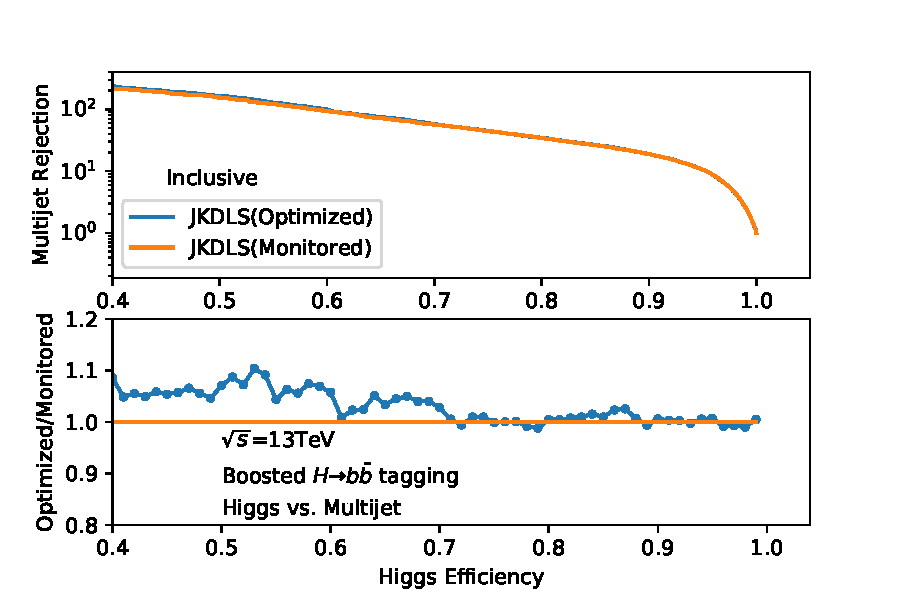
\includegraphics[width=0.75\textwidth]{figuresXbb/OPT/OPTQCD.pdf}
  % \caption{Higgs vs. Multijet, inclusive}
   \caption{}
   %\label{fig:}
  \end{subfigure}
  \begin{subfigure}{.5\textwidth}
  \centering
   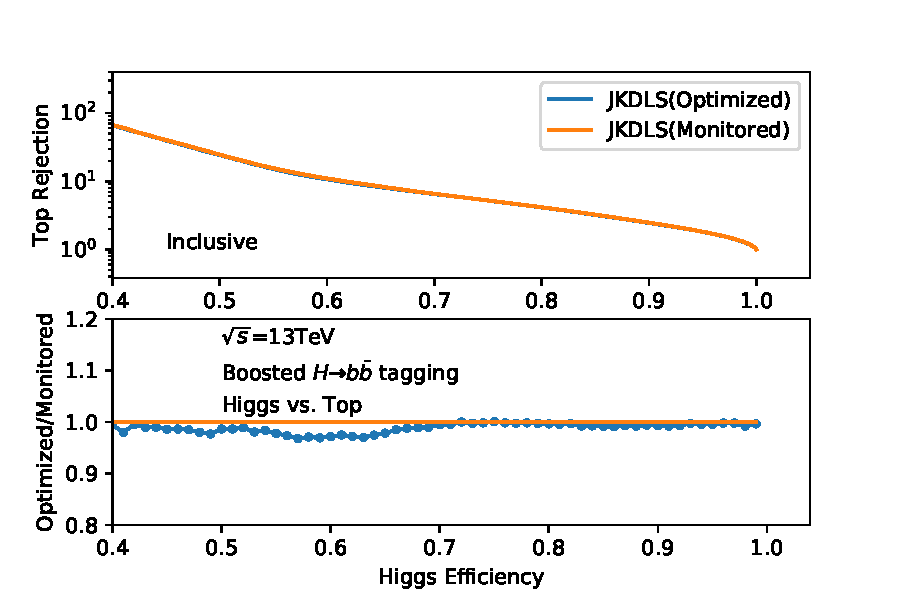
\includegraphics[width=0.75\textwidth]{figuresXbb/OPT/OPTop.pdf}
   %\caption{Higgs vs. Top, Inclusive}
    \caption{}
   %\label{fig:}
  \end{subfigure}
\newline 
   \begin{subfigure}{.5\textwidth}
  \centering
   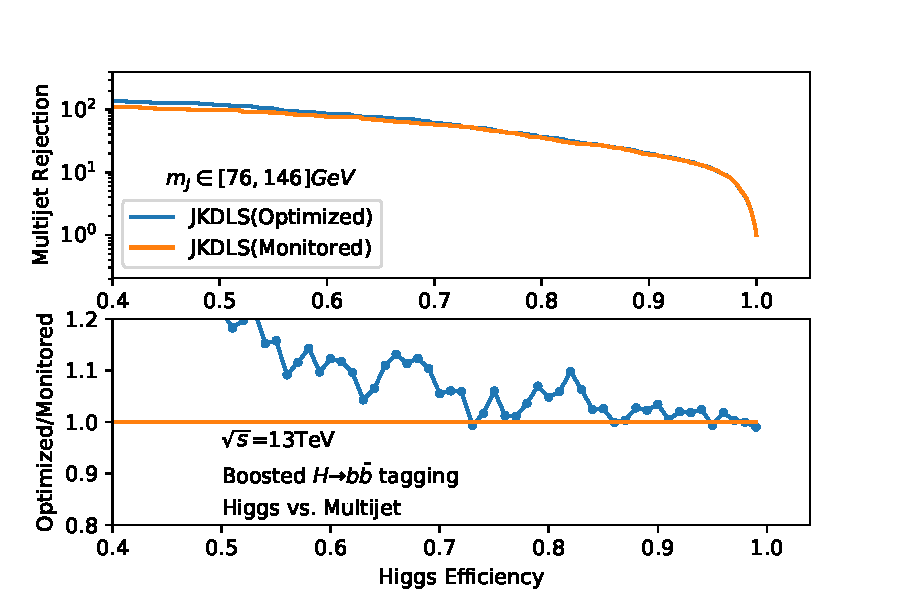
\includegraphics[width=0.75\textwidth]{figuresXbb/OPT/OPTQCDMASS.pdf}
  % \caption{Higgs vs. Multijet, $m_{J}\in [76,146]GeV$}
    \caption{}
   %\label{fig:}
  \end{subfigure}
  \begin{subfigure}{.5\textwidth}
  \centering
   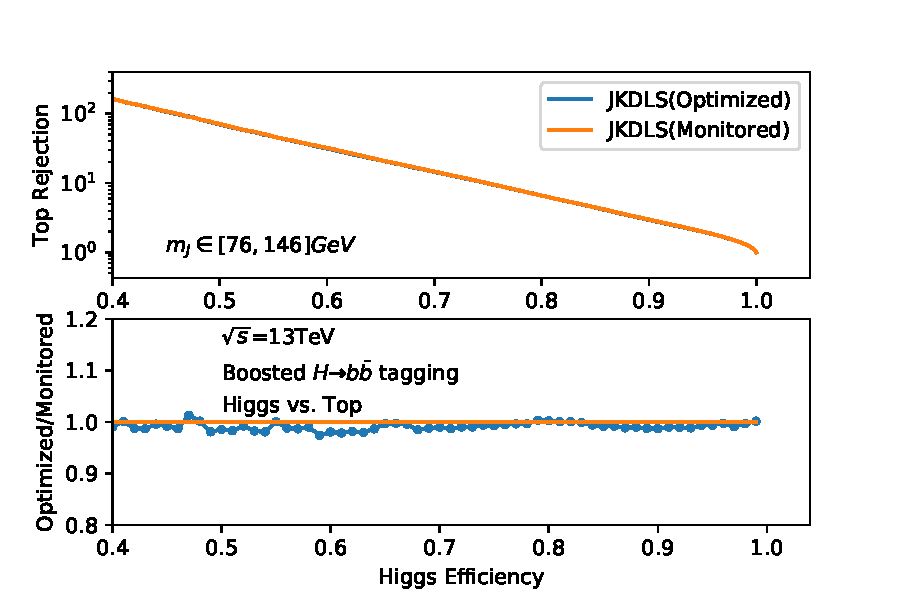
\includegraphics[width=0.75\textwidth]{figuresXbb/OPT/OPTopMASS.pdf}
  % \caption{Higgs vs. Top, $m_{J}\in [76,146]GeV$}
    \caption{}
   %\label{fig:}
  \end{subfigure}
 \newline 
   \begin{subfigure}{.5\textwidth}
  \centering
   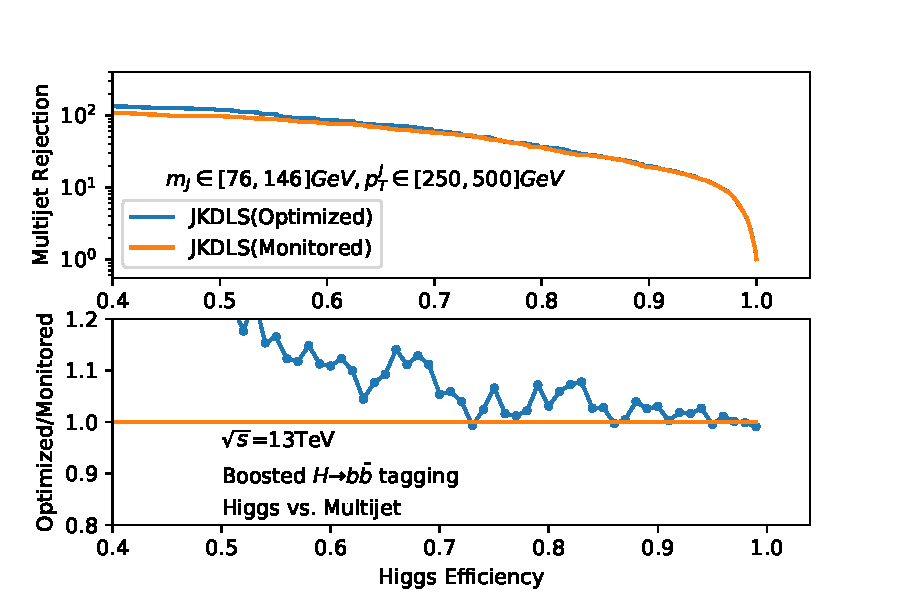
\includegraphics[width=0.75\textwidth]{figuresXbb/OPT/OPTQCDMASSPT1.pdf}
  % \caption{Higgs vs. Multijet, $m_{J}\in [76,146]GeV, p_{T}^{J}\in [250,500]GeV$}
    \caption{}
   %\label{fig:}
  \end{subfigure}
  \begin{subfigure}{.5\textwidth}
  \centering
   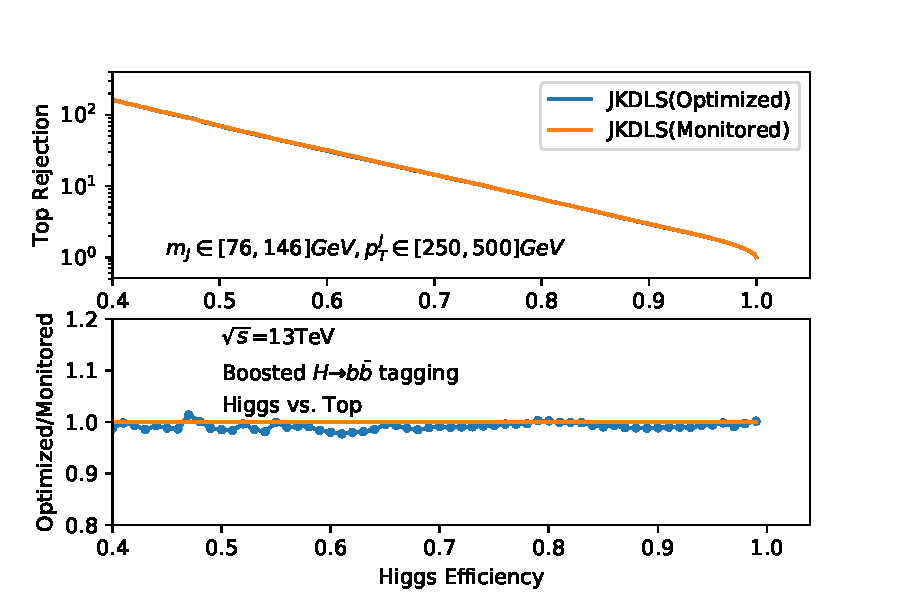
\includegraphics[width=0.75\textwidth]{figuresXbb/OPT/OPTopMASSPT1.pdf}
   %\caption{Higgs vs. Top, $m_{J}\in [76,146]GeV, p_{T}^{J}\in [250,500]GeV$}
    \caption{}
   %\label{fig:}
  \end{subfigure}
 \newline 
   \begin{subfigure}{.5\textwidth}
  \centering
   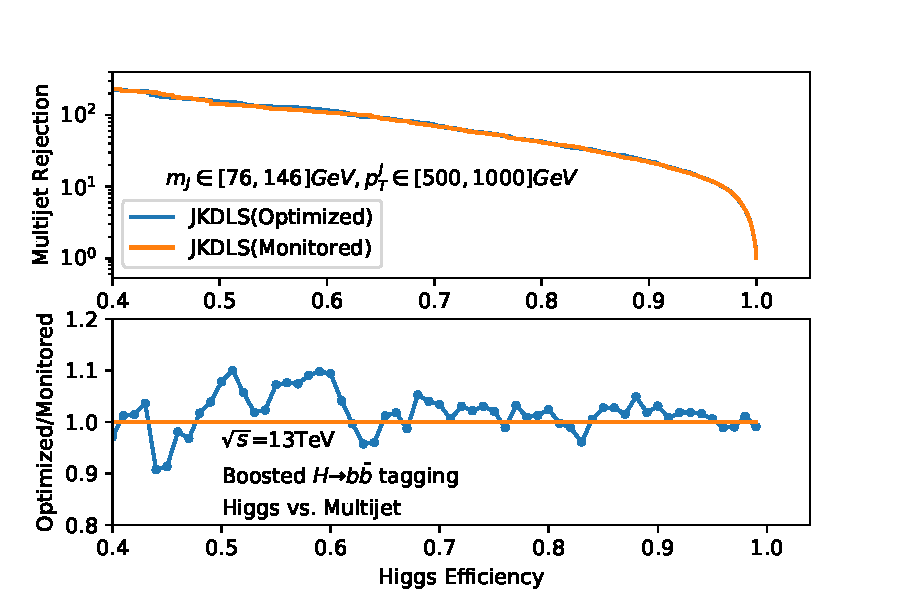
\includegraphics[width=0.75\textwidth]{figuresXbb/OPT/OPTQCDMASSPT2.pdf}
  % \caption{Higgs vs. Multijet, $m_{J}\in [76,146]GeV, p_{T}^{J}\in [500,1000]GeV$}
    \caption{}
   %\label{fig:}
  \end{subfigure}
  \begin{subfigure}{.5\textwidth}
  \centering
   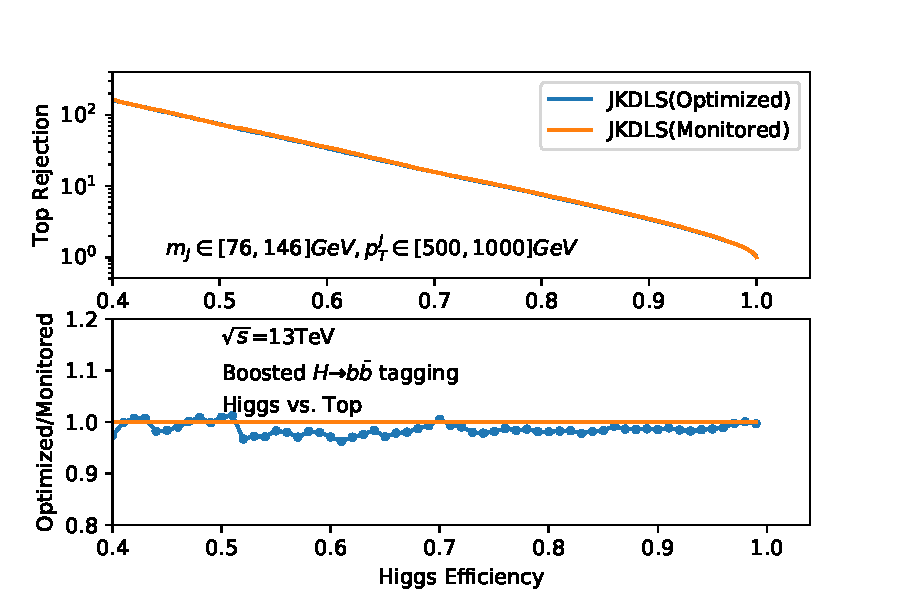
\includegraphics[width=0.75\textwidth]{figuresXbb/OPT/OPTopMASSPT2.pdf}
   %\caption{Higgs vs. Top, $m_{J}\in [76,146]GeV, p_{T}^{J}\in [500,1000]GeV$}
    \caption{}
   %\label{fig:}
  \end{subfigure}
 \newline 
   \begin{subfigure}{.5\textwidth}
  \centering
   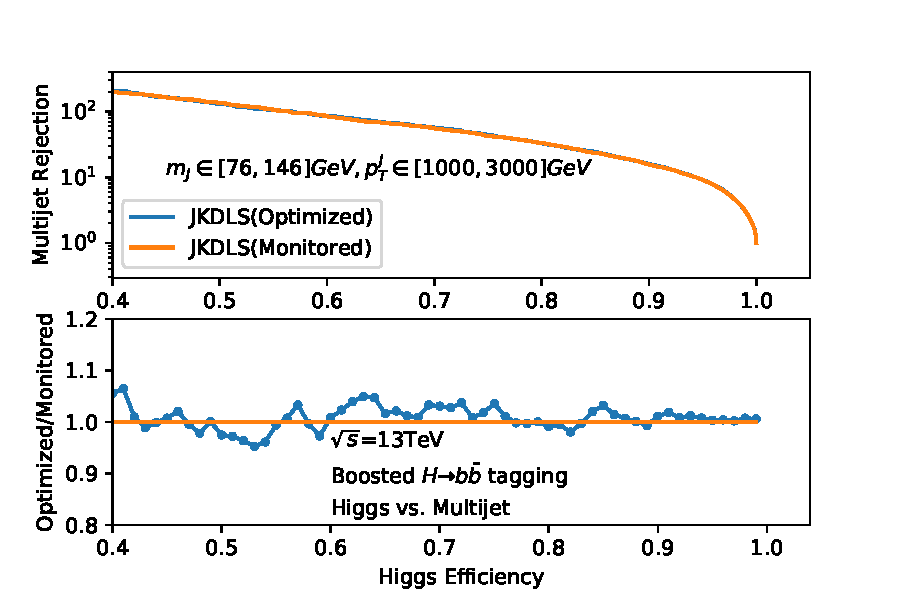
\includegraphics[width=0.75\textwidth]{figuresXbb/OPT/OPTQCDMASSPT3.pdf}
  % \caption{Higgs vs. Multijet, $m_{J}\in [76,146]GeV, p_{T}^{J}\in [1000,3000]GeV$}
    \caption{}
   %\label{fig:}
  \end{subfigure}
  \begin{subfigure}{.5\textwidth}
  \centering
   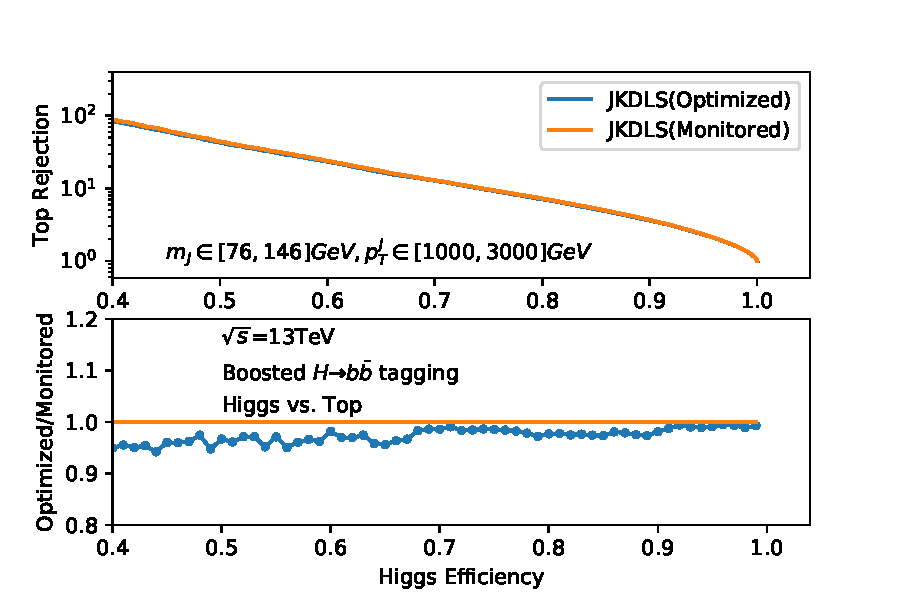
\includegraphics[width=0.75\textwidth]{figuresXbb/OPT/OPTopMASSPT3.pdf}
  % \caption{Higgs vs. Top, $m_{J}\in [76,146]GeV, p_{T}^{J}\in [1000,3000]GeV$}
    \caption{}
   %\label{fig:}
  \end{subfigure}
  \caption{
对照组和优化组的模型的性能对比。
左排的图展示的是multijet本底排除率随着信号效率的变化关系对比,
右排的图展示的是t夸克本底排除率随着信号效率的变化关系对比,
从上到下依次对应于第~\ref{sec:XbbTagger25}~小节中定义的五个区间。
%左边的图展示的是multijet本底排除率与信号效率的变化关系的对比,
%右边的图展示的是t夸克本底排除率与信号效率的变化关系的对比,
%从上到下依次对应于五个区间的性能对比。
  }
  \label{fig:OPTROC}
\end{figure} 


综上所述,
基于神经网络,
我们用变量控制的方法成功实现了新算法的去质量关联,
而且新算法的性能在一定程度上得到了提升,
表~\ref{tab:Final}~是
用于新算法训练的结构参数以及输入变量和加权策略。
%算法训练最终的结构参数以及输入变量和加权策略。
下一小节将会看到,
%对比
与ATLAS合作组目前所使用的基线算法相比,
%设计出来的
新算法显著提高了来自高横动量$H\rightarrow b\bar{b}$事例与来自QCD过程的multijet事例和来自强子型衰变的t夸克事例的
区分精度。
%区分度。

\begin{table}[ht]
\caption{
%算法训练最终的结构参数以及输入变量和加权策略。
新算法训练的结构参数以及输入变量和加权策略。
}
\begin{center}
%\begin{adjustbox}{width=\columnwidth,center}
\begin{tabular}{c|c}
    \hline
    \hline
    Parameter & Value or type  \\
    \hline  
    Loss & Categorical crossentropy \\
     \hline  
    Optimizer & \textsc{Adam}~\cite{Kingma:2014} \\
    \hline  
    Hidden layers & 6 \\
    \hline  
    Nodes per hidden layers & 250 \\
    \hline  
    Learning rate & $10^{-2}$\\
    \hline  
    Learning rate decay & $10^{-5}$ \\
    \hline  
    Activation of inner layers & \textsc{ReLU}~\cite{Glorot:2011} \\
    \hline  
    Activation of outer layers & \textsc{SoftMax}~\cite{MLMIT} \\
    \hline  
    Batch normalization~\cite{Ioffe:2015} & $10^{4}$ \\
    \hline  
    Epoch & 200 \\
    \hline  
    Inputs & JK from LR-jet + DLS from VR-jet \\
    \hline  
    Weighting strategy & resampling \\
    \hline
    \hline
\end{tabular}
%\end{adjustbox}
\end{center}
\label{tab:Final}
\end{table}


\section{算法性能}
\label{sec:XbbPerf}


通过\textsc{Lwtnn}~\cite{lwtnn}将上一小节
%设计出来
的高横动量$H\rightarrow b\bar{b}$标定算法
%应用
合并到ATLAS合作组内部的软件系统中之后,
我们将其性能与ATLAS合作组
%内部现在
目前所使用的基线算法的性能做了详细对比。
%LR-jet来自
新算法$D_{Xbb}$的区分因子是通过
%模型
它的三个输出变量$p_{\text{Higgs}}$、$p_{\text{multijet}}$和$p_{\text{top}}$
来定义的:
%用以下式子来定义:
\begin{equation} 
\label{eq:discr}
D_{Xbb} = \ln\frac{p_{\text{Higgs}}}{f_{Top}\cdot p_{\text{top}} + (1-f_{Top})\cdot p_{\text{multijet}}} %prob need a better name for this variable
\end{equation}
其中$f_{Top}$决定了t夸克本底的比例,
%在本章的性能研究当中,我们将它固定为
在这一小节的研究当中,取$f_{Top}=0.25$。
%可以通过调整上式中区分因子的定义方式在比例不同的样本中筛选三种样本中任意一种,
%而
新算法的工作点是通过在区分因子$D_{Xbb}$上的一个截断值来定义的,
所选择的截断值对应于
它在信号样本中对Higgs-jet事例的一个特定的标定效率,
%在信号样本中它对Higgs-jet事例的一个特定的标定效率,
其中信号样本是
满足第~\ref{sec:XbbOR}~小节中筛选条件的样本。
%应用第~\ref{sec:XbbOR}~小节筛选条件后的样本。
而ATLAS合作组的基线算法由DL1r和MV2提供,
定义方式与上一轮研究~\cite{TAGGING5}类似,
%基线算法
DL1r或MV2要求LR-jet中包含至少两个subjet,
对于
%前
其中两个横动量最高的subjet,
由DL1r或MV2提供的区分因子都要高于某个给定的阈值,
%由DL1r或MV2算法输出的用于b-jet标定的区分因子都要高于某个给定的阈值,
也就是对应于这两个subjet的区分因子中最小的那个要高于某一阈值,
满足上述条件的LR-jet才会被
%基线算法
DL1r或MV2标定为Higgs-jet。
%另外,为了更好的测试算法性能,除了第~\ref{sec:XbbOR}~小节描述的筛选条件之外,
%我们还要求事例中领头LR-jet的质量在76GeV和146GeV之间,
%因为在上一轮研究~\cite{TAGGING5}当中,
%在LR-jet横动量大于250GeV的情况下,
%这个质量区间所包含的Higgs-jet的数量占总数的90\%。

\subsection{去质量关联}
\label{sec:XbbPerf1}
首先,我们对$D_{Xbb}$算法与事例中领头LR-jet质量的关联性进行了研究,
在这一小节的研究当中,对于t夸克样本中,没有要求事例中至少包含一个Top-jet,
其他要求没有改变。
在$D_{Xbb}$算法的标定效率为60\%的工作点下,
如图~\ref{fig:MASS1}~所示,我们对比了事例中领头LR-jet质量分布在$D_{Xbb}$标定之前和之后的分布,
左图是信号样本和multijet样本中领头LR-jet质量分布在$D_{Xbb}$标定之前和之后的对比,
而右图是信号样本和t夸克样本中领头LR-jet质量分布在$D_{Xbb}$标定之前和之后的对比,
可以看到$D_{Xbb}$算法对LR-jet的质量分布影响非常小。

\begin{figure}[h]
  \begin{center}
    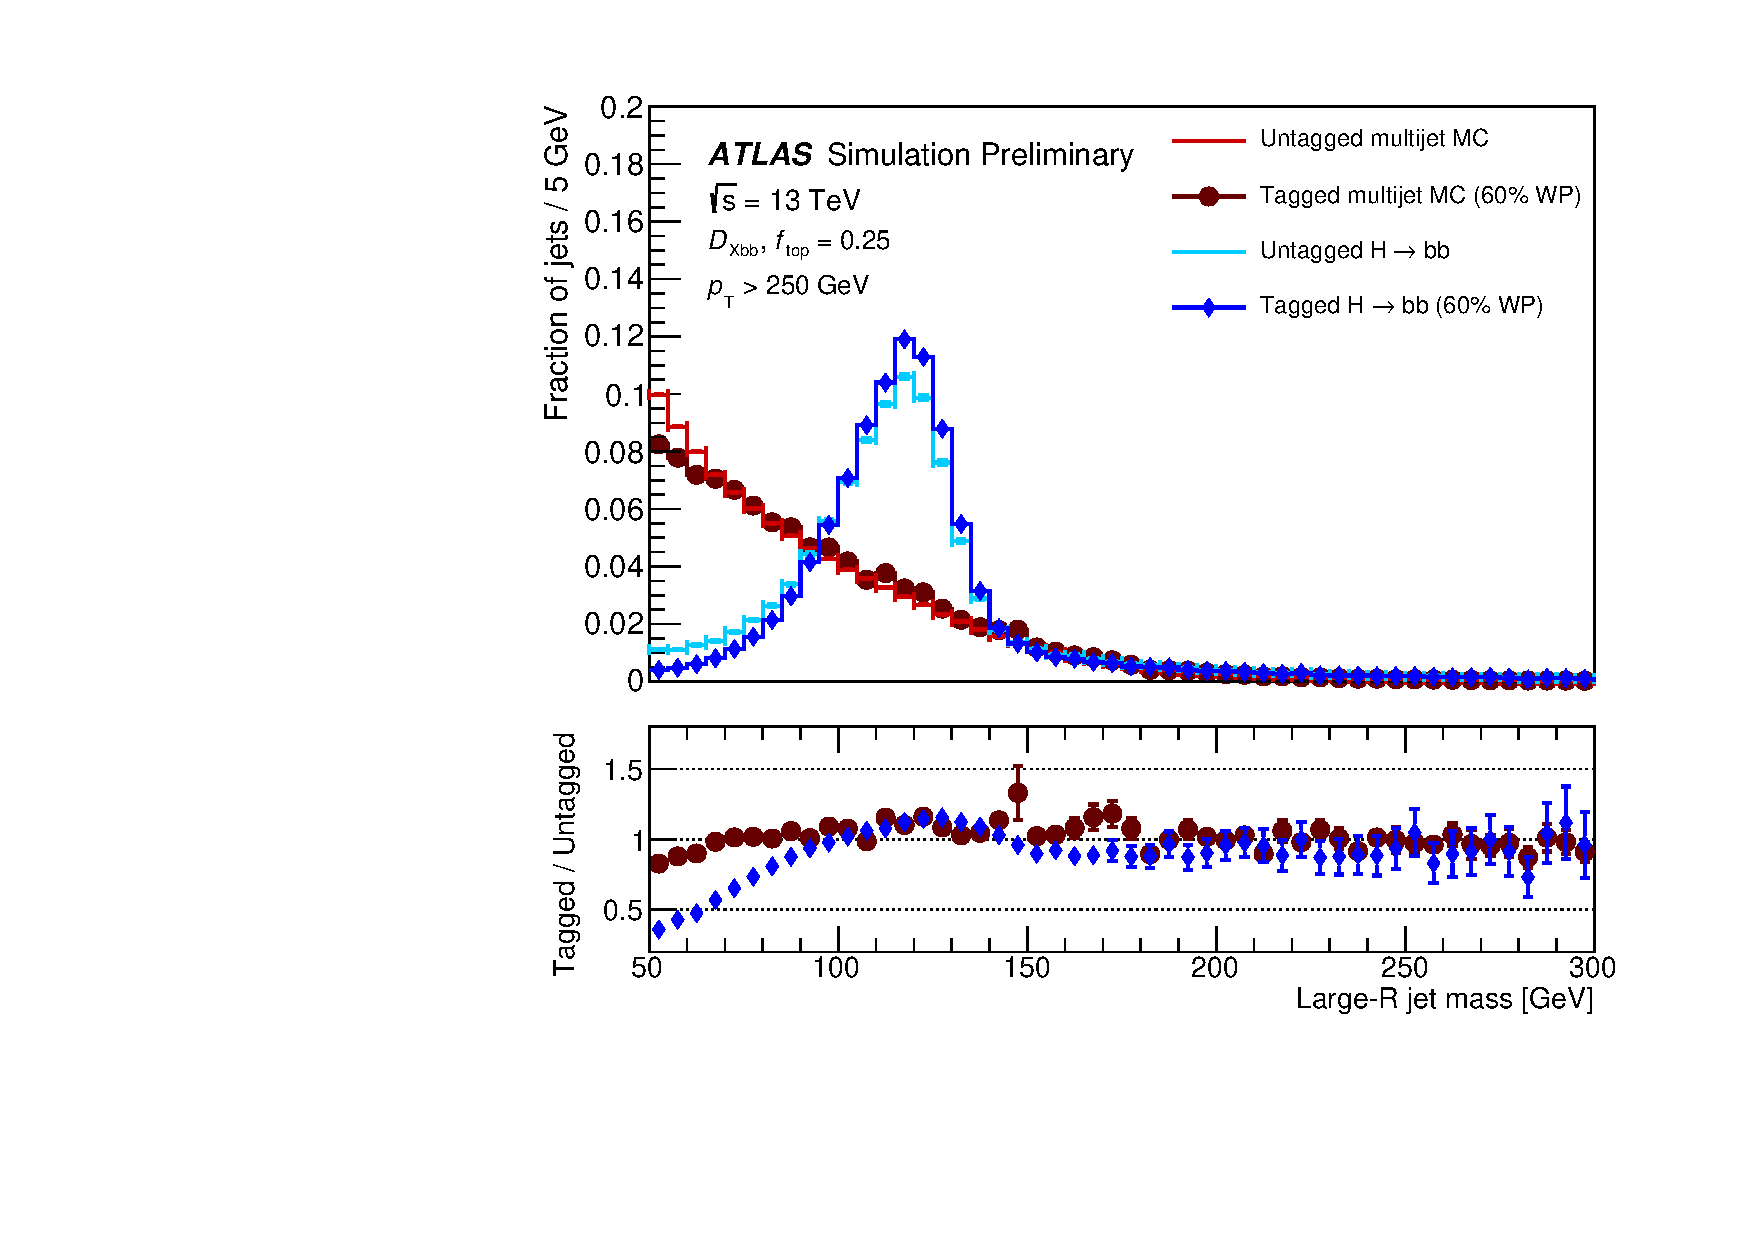
\includegraphics[width=0.49\textwidth]{figuresXbb/efficiencies/dijetcomp_all_largeRjet_jetjet_JZ_mass_inclusive_discf025zoom.pdf}
    \includegraphics[width=0.49\textwidth]{figuresXbb/efficiencies/ttcomp_all_largeRjet_tt_mass_inclusive_discf025zoom.pdf}
  \end{center}
  \caption{
 在$D_{Xbb}$算法的标定效率为60\%的工作点下,事例中领头LR-jet质量分布在$D_{Xbb}$标定之前和之后的分布对比。
 左图是信号样本和multijet样本中领头LR-jet质量分布在$D_{Xbb}$标定之前和之后的对比,
右图是信号样本和t夸克样本中领头LR-jet质量分布在$D_{Xbb}$标定之前和之后的对比。
}
  \label{fig:MASS1}
\end{figure}


同样在基线算法DL1r的标定效率为60\%的工作点下,
如图~\ref{fig:MASS2}~所示,我们还研究了基线算法DL1r对事例中领头LR-jet质量分布的影响,
左图是对于multijet样本,右图是对于t夸克样本,
可以看到基线算法DL1r对LR-jet的质量分布影响也非常小,这是我们所预期的。

\begin{figure}[h]
  \begin{center}
    \includegraphics[width=0.49\textwidth]{figuresXbb/efficiencies/dijetcomp_all_largeRjet_jetjet_JZ_mass_inclusive_discDL1rBaselinezoom.pdf}
    \includegraphics[width=0.49\textwidth]{figuresXbb/efficiencies/ttcomp_all_largeRjet_tt_mass_inclusive_discDL1rBaselinezoom.pdf}
  \end{center}
  \caption{事例中领头LR-jet质量分布在基线算法DL1r标定之前和之后的分布对比。
 左图是信号样本和multijet样本中领头LR-jet质量分布被基线算法DL1r标定之前和之后的对比,
 右图是信号样本和t夸克样本中领头LR-jet质量分布被基线算法DL1r标定之前和之后的对比。}
  \label{fig:MASS2}
\end{figure}

为了进一步说明$D_{Xbb}$算法对LR-jet质量分布的影响足够小,
如图~\ref{fig:MASS3}~所示,
我们还对比了事例中领头LR-jet质量分布在$D_{Xbb}$和基线算法DL1r标定之后的分布,
图~\ref{fig:MASS3QCD}~是对于multijet样本,图~\ref{fig:MASS3Top}~是对于t夸克样本,图~\ref{fig:MASS3Higgs}~是对于信号样本,
可以看到两者的差异都非常小,这是我们所能接受的。


\begin{figure}[!thbp]
  \begin{subfigure}{.5\textwidth}
  \centering
  \includegraphics[width=0.9\textwidth]{figuresXbb/efficiencies/jetjet_JZsculpt_all_largeRjet_mass_inclusive_discf025zoom.pdf}
  \caption{}
  \label{fig:MASS3QCD}
  \end{subfigure}
  \begin{subfigure}{.5\textwidth}
  \centering
  \includegraphics[width=0.9\textwidth]{figuresXbb/efficiencies/ttsculpt_all_largeRjet_mass_inclusive_discf025zoom.pdf}
  \caption{}
  \label{fig:MASS3Top}
  \end{subfigure}
\newline 
  \begin{subfigure}{.99\textwidth}
  \centering
  \includegraphics[width=0.5\textwidth]{figuresXbb/efficiencies/RS_G_hh_bbbbsculpt_all_largeRjet_mass_inclusive_discf025zoom.pdf}
  \caption{}
  \label{fig:MASS3Higgs}
  \end{subfigure}
  \caption{
 事例中领头LR-jet质量分布在$D_{Xbb}$和基线算法DL1r标定之后的分布对比。
 (a) 对于multijet样本;(b) 对于t夸克样本;(c) 对于信号样本。
 }
\label{fig:MASS3}
\end{figure}



\subsection{味标签}
\label{sec:XbbPerf2}

%由于信号样本是由KK $G\to hh$产生,
%由大质量的引力子衰变而来的两个希格斯玻色子在探测器模拟中产生的两个LR-jet可能发生重叠,
%这使得信号样本中领头LR-jet包含三个subjet的事例比例比较高。

为了更好的测试算法性能,除了第~\ref{sec:XbbOR}~小节描述的筛选条件之外,
我们还要求事例中领头LR-jet的质量在76GeV和146GeV之间,
这个质量区间所包含的Higgs-jet的数量占总数的90\%~\cite{TAGGING5}。
应用了全部筛选条件之后,我们对样本的多样性和其中真实味标签的分布进行了研究,
表~\ref{tab:XbbPerf1}~展示了三个样本中事例领头LR-jet的VR-jet个数多样性,
信号样本和t夸克样本中有超过99\%的事例中领头LR-jet包含至少两个VR-jet,
而multijet样本中约有97.5\%的事例中领头LR-jet包含至少两个VR-jet。

\begin{table}
\begin{center}
  \begin{tabular}{ c|c c c }
    \hline
    \hline
    Category & Multijet & Top & Higgs \\
    \hline
    = 1 VR-jet  & 0.025  & 0.009  & 0.005 \\ 
    \hline
    = 2 VR-jet & 0.469  & 0.463  & 0.585 \\ 
    \hline
    $\geq$ 3 VR-jet & 0.505  & 0.528  & 0.410 \\ 
    \hline
    \hline
  \end{tabular}
  \caption{
  应用事例筛选条件之后,三个样本中事例领头LR-jet的VR-jet个数多样性。
      }
\label{tab:XbbPerf1}
\end{center}
\end{table}

表~\ref{tab:XbbPerf2}~展示了三个样本中事例领头LR-jet的VR-jet真实味标签的分布,
可以看到,信号样本中约有92\%的事例有如下特点,其中领头LR-jet包含至少两个真实味标签为b-jet的VR-jet,
在multijet样本中,大约有80\%的事例中领头LR-jet既不包含真实味标签为b-jet的VR-jet也不包含真实味标签为c-jet的VR-jet,
而t夸克样本主要由领头LR-jet中包含单个真实味标签为b-jet的VR-jet的事例主导,
这是由t夸克的性质决定的~\cite{PDG}。


\begin{table}
\begin{center}
  \begin{tabular}{ c|c c c }
    \hline
    \hline
    Category & Multijet & Top & Higgs \\
    \hline
    $\geq2b$ & 0.022 & 0.019 & 0.922 \\
    \hline
    $1b \ + \geq1c$ & 0.005 & 0.221 & 0.007 \\
    \hline
    $1b \ + \ 0c $ & 0.039 & 0.481 & 0.070 \\
    \hline
    $0b \ + \geq2c$ & 0.036 & 0.007 & - \\
    \hline
    $0b \ + \ 1c$ & 0.098 & 0.109 & - \\
    \hline
    $0b \ + \ 0c$ & 0.801 & 0.162 & 0.001 \\
    \hline
    \hline
  \end{tabular}
  \caption{
 应用事例筛选条件之后,三个样本中事例领头LR-jet的VR-jet真实味标签的分布。
  }
\label{tab:XbbPerf2}
\end{center}
\end{table}


为了测试$D_{Xbb}$的作用效果,在$D_{Xbb}$算法的标定效率为60\%的工作点下,
我们研究了被$D_{Xbb}$标定之后的样本中事例领头LR-jet的VR-jet真实味标签的分布,
如表~\ref{tab:XbbPerf3}~所示,对比标定之前表~\ref{tab:XbbPerf2}~的情形,
multijet样本和t夸克样本中具有以下特点的事例比例得到了显著的提升,
领头LR-jet包含至少一个真实味标签为b-jet的VR-jet,
分别达到了约95\%和99\%,
也就是$D_{Xbb}$可以有效的排除领头LR-jet中VR-jet真实味标签为light-jet的事例。

\begin{table}
\begin{center}
  \begin{tabular}{ c|c c c }
    \hline
    \hline
    Category & Multijet & Top & Higgs \\
    \hline
$\geq2b$ & 0.871 & 0.229 & 0.997 \\
 \hline
$1b + \geq1c$ & 0.041 & 0.551 & 0.001 \\
 \hline
$1b + 0c $ & 0.046 & 0.216 & 0.002 \\
 \hline
$\geq2c + 0b$ & 0.033 & 0.001 & - \\
 \hline
$1c + 0b$ & 0.008 & 0.003 & - \\
 \hline
$0b + 0c$ & 0.002 & - & - \\
    \hline
    \hline
  \end{tabular}
  \caption{
  在$D_{Xbb}$算法的标定效率为60\%的工作点下,
被$D_{Xbb}$标定之后的样本中事例领头LR-jet的VR-jet真实味标签的分布。
  }
  \label{tab:XbbPerf3}
  \end{center}
\end{table}

\subsection{区分因子}
\label{sec:XbbPerf3}

在区分因子对比之前,
我们先研究了
%基线算法
DL1r的三个输出值$p_b$、$p_c$和$p_u$在样本中的分布,
%它们分别代表jet被判定为b-jet、c-jet或者除前两者之外的light-jet的概率,
以及$D_{Xbb}$的三个输出值$p_{\text{Higgs}}$、$p_{\text{multijet}}$和$p_{\text{top}}$在样本中的分布:
%它们分别代表事例是来自Higgs-jet、QCD-jet和Top-jet事例的概率:
\begin{itemize}
\item 图~\ref{fig:DL1RLD}~分别展示了在信号样本、multijet样本和t夸克样本中,
DL1r的三个输出在领头LR-jet中领头VR-jet中的分布。
%领头LR-jet中领头VR-jet的
%DL1r算法
%三个输出值$p_b$、$p_c$和$p_u$的分布。
其中左图代表$p_b$的分布,中间的图代表$p_c$的分布,右图代表$p_u$的分布,橙色线代表信号样本,蓝色线代表multijet样本,绿色线代表t夸克样本。
所有分布都已经归一化。
\item 图~\ref{fig:DL1RLLD}~分别展示了在信号样本、multijet样本和t夸克样本中,
DL1r的三个输出在领头LR-jet中次领头也就是横动量第二高的VR-jet中的分布。
%领头LR-jet中次领头也就是横动量第二高的VR-jet的
%DL1r算法
%三个输出值$p_b$、$p_c$和$p_u$的分布。

%\item 图~\ref{fig:DL1RLLLD}~分别展示了在信号样本、multijet样本和t夸克样本中,
%DL1r的三个输出在领头LR-jet中次领头也就是横动量第三高的VR-jet中的分布。

%领头LR-jet中次次领头也就是横动量第三高的VR-jet的
%DL1r算法
%三个输出值$p_b$、$p_c$和$p_u$的分布。

\item 图~\ref{fig:DXBBPP}~分别展示了在信号样本、multijet样本和t夸克样本中,
$D_{Xbb}$的三个输出在领头LR-jet中的分布。
%领头LR-jet的三个输出值$p_{\text{Higgs}}$、$p_{\text{multijet}}$和$p_{\text{top}}$的分布。
其中左图代表$p_{\text{Higgs}}$的分布,中间的图代表$p_{\text{multijet}}$的分布,右图代表$p_{\text{top}}$的分布,橙色线代表信号样本,蓝色线代表multijet样本,绿色线代表t夸克样本。
%所有分布都已经归一化。
\end{itemize}

%从图中对比可以看到,新算法的输出值在三个样本中的分布差异比较显著。

\begin{figure}[h]
    \includegraphics[width=0.33\textwidth]{figuresXbb/samples/inputs_aux/dl1r_pb_1_norm.pdf}
    \includegraphics[width=0.33\textwidth]{figuresXbb/samples/inputs_aux/dl1r_pc_1_norm.pdf}
    \includegraphics[width=0.33\textwidth]{figuresXbb/samples/inputs_aux/dl1r_pu_1_norm.pdf}
  \caption{
  在信号样本、multijet样本和t夸克样本中,DL1r的三个输出值$p_b$、$p_c$和$p_u$在领头LR-jet中领头VR-jet中的分布。
  %在信号样本、multijet样本和t夸克样本中,领头LR-jet中的领头VR-jet的DL1r算法输出值$p_b$、$p_c$和$p_u$的分布。
其中左图代表$p_b$的分布,中间的图代表$p_c$的分布,右图代表$p_u$的分布,橙色线代表信号样本,蓝色线代表multijet样本,绿色线代表t夸克样本。
}
  \label{fig:DL1RLD}
\end{figure}

\begin{figure}[h]
    \includegraphics[width=0.33\textwidth]{figuresXbb/samples/inputs_aux/dl1r_pb_2_norm.pdf}
    \includegraphics[width=0.33\textwidth]{figuresXbb/samples/inputs_aux/dl1r_pc_2_norm.pdf}
    \includegraphics[width=0.33\textwidth]{figuresXbb/samples/inputs_aux/dl1r_pu_2_norm.pdf}
  \caption{
  在信号样本、multijet样本和t夸克样本中,
DL1r的三个输出值$p_b$、$p_c$和$p_u$在领头LR-jet中次领头也就是横动量第二高的VR-jet中的分布。
  %在信号样本、multijet样本和t夸克样本中,领头LR-jet中的次领头也就是横动量第二高的VR-jet的DL1r算法输出值$p_b$、$p_c$和$p_u$的分布。
其中左图代表$p_b$的分布,中间的图代表$p_c$的分布,右图代表$p_u$的分布,橙色线代表信号样本,蓝色线代表multijet样本,绿色线代表t夸克样本。
}
\label{fig:DL1RLLD}
\end{figure}

\begin{comment}
\begin{figure}[h]
    \includegraphics[width=0.33\textwidth]{figuresXbb/samples/inputs_aux/dl1r_pb_3_norm.pdf}
    \includegraphics[width=0.33\textwidth]{figuresXbb/samples/inputs_aux/dl1r_pc_3_norm.pdf}
    \includegraphics[width=0.33\textwidth]{figuresXbb/samples/inputs_aux/dl1r_pu_3_norm.pdf}
  \caption{
  在信号样本、multijet样本和t夸克样本中,
DL1r的三个输出值$p_b$、$p_c$和$p_u$在领头LR-jet中次领头也就是横动量第三高的VR-jet中的分布。
  %在信号样本、multijet样本和t夸克样本中,领头LR-jet中的次次领头也就是横动量第三高的VR-jet的DL1r算法输出值$p_b$、$p_c$和$p_u$的分布。
其中左图代表$p_b$的分布,中间的图代表$p_c$的分布,右图代表$p_u$的分布,橙色线代表信号样本,蓝色线代表multijet样本,绿色线代表t夸克样本。
}
\label{fig:DL1RLLLD}
\end{figure}
\end{comment}


\begin{figure}[h]
    \includegraphics[width=0.33\textwidth]{figuresXbb/samples/probs_aux/Xbb_Higgs_norm.pdf}
    \includegraphics[width=0.33\textwidth]{figuresXbb/samples/probs_aux/Xbb_QCD_norm.pdf}
    \includegraphics[width=0.33\textwidth]{figuresXbb/samples/probs_aux/Xbb_Top_norm.pdf}
  \caption{
  在信号样本、multijet样本和t夸克样本中,$D_{Xbb}$的三个输出值$p_{\text{Higgs}}$、$p_{\text{multijet}}$和$p_{\text{top}}$在领头LR-jet中的分布。
 % 在信号样本、multijet样本和t夸克样本中,领头LR-jet中的新算法输出值$p_{\text{Higgs}}$、$p_{\text{multijet}}$和$p_{\text{top}}$的分布。
其中左图代表$p_{\text{Higgs}}$的分布,中间的图代表$p_{\text{multijet}}$的分布,右图代表$p_{\text{top}}$的分布,橙色线代表信号样本,蓝色线代表multijet样本,绿色线代表t夸克样本。
}
  \label{fig:DXBBPP}
\end{figure}



接下来我们对比了$D_{Xbb}$算法和DL1r基线算法在样本中的区分因子的分布。
如图~\ref{fig:XbbPerf3}~所示,左图~\ref{fig:XbbPerf3DXBB}展示的是,
在信号样本、multijet样本和t夸克样本中,
由$D_{Xbb}$算法输出的的LR-jet的区分因子的分布,
分别以橙色、蓝色和绿色线表示;
而右图~\ref{fig:XbbPerf3DL1r}~展示的是,
在信号样本、multijet样本和t夸克样本中,
由基线算法DL1r输出的LR-jet的区分因子的分布,
也是分别以橙色、蓝色和绿色线表示。
可以看出,相比之下,
$D_{Xbb}$算法能将信号和两种本底比较明显的区分开。

\begin{figure}[!thbp]
  \begin{subfigure}{.5\textwidth}
  \centering
  \includegraphics[width=0.9\textwidth]{figuresXbb/samples/Hbb_025_norm.pdf}
  \caption{}
  \label{fig:XbbPerf3DXBB}
  \end{subfigure}
  \begin{subfigure}{.5\textwidth}
  \centering
  \includegraphics[width=0.9\textwidth]{figuresXbb/samples/dl1r_norm.pdf}
  \caption{}
  \label{fig:XbbPerf3DL1r}
  \end{subfigure}
  \caption{
  在信号样本、multijet样本和t夸克样本中,由$D_{Xbb}$算法(左图)和基线算法DL1r(右图)输出的LR-jet的区分因子的分布,分别以橙色、蓝色和绿色线表示。
  其中分布都已经归一化。
 }
\label{fig:XbbPerf3}
\end{figure}


\subsection{本底排除率与信号效率}
\label{sec:XbbPerf4}

%在对$D_{Xbb}$算法性能进行评估的时候,~\ref{sec:XbbOR}小节所提到的筛选条件和~\ref{sec:XbbTagger}小节定义的希格斯玻色子质量区间都应用了,而且信号样本和t夸克样本都被重新加权,使得这两种样本中的大半径jet的横动量分布和图~\ref{fig:bkg-pt}中multijet样本中大半径jet的横动量分布是一样的。

然后我们对比了在区分因子取不同截断值的情况下,$D_{Xbb}$算法与基线算法DL1r和MV2的本底排除率随着信号效率的变化关系。
如图~\ref{fig:roc250}~所示,分别对multijet本底和t夸克本底进行了评估,
蓝色线代表$D_{Xbb}$的性能,绿色线和灰色线分别代表基线算法DL1r和MV2基于领头LR-jet中两个横动量最高的VR-jet的性能表现,
而灰色虚线代表基线算法MV2基于领头LR-jet中两个横动量最高的FR-jet的性能表现,
图中底部展示的是信号效率相同时,各算法的本底排除率与基于VR-jet的基线算法MV2的本底排除率的比值,
可以看出在信号效率相同的情况下,$D_{Xbb}$算法能实现相同或相对更高的本底排除率,尤其是在高信号效率区间。

\begin{figure}[!thbp]
  \begin{subfigure}{.5\textwidth}
  \centering
  \includegraphics[width=0.9\textwidth]{figuresXbb/pulled/roc/250_inf/zoom/dijet.pdf}
  \caption{Higgs vs. Multijet}
  \end{subfigure}
  \begin{subfigure}{.5\textwidth}
  \centering
  \includegraphics[width=0.9\textwidth]{figuresXbb/pulled/roc/250_inf/top.pdf}
  \caption{Higgs vs. Top}
  \end{subfigure}
  \caption{
在领头LR-jet满足$p_{T}$>250GeV时,$D_{Xbb}$算法与基线算法DL1r和MV2的本底排除率随着信号效率的变化关系。
分别对multijet本底(左图)和t夸克本底(右图)进行了评估。
蓝色线代表$D_{Xbb}$的性能,绿色线和灰色线分别代表基线算法DL1r和MV2基于领头LR-jet中两个横动量最高的VR-jet的性能表现,
而灰色虚线代表基线算法MV2基于领头LR-jet中两个横动量最高的FR-jet的性能表现。
图中底部展示的是信号效率相同时,各算法的本底排除率与基于VR-jet的基线算法MV2的本底排除率的比值。
 }
\label{fig:roc250}
\end{figure}

为了凸显$D_{Xbb}$算法在高横动量区间的性能优势,
在增加样本中领头LR-jet横动量大于500GeV的筛选条件之后,
我们重新评估了$D_{Xbb}$算法与基线算法DL1r和MV2的本底排除率随着信号效率的变化。
如图~\ref{fig:roc500}~所示,同样分别对multijet本底和t夸克本底进行了评估,
可以看到,在信号效率为$60\%$的情况下,
对于multijet本底,$D_{Xbb}$的本底排除率达到了92,是基于VR-jet的基线算法MV2的本底排除率的1.4倍,
与基于VR-jet的基线算法DL1r的本底排除率大致相等;
对于t夸克本底,$D_{Xbb}$的本底排除率达到了31,是基于VR-jet的基线算法MV2的本底排除率的2倍,
是基于VR-jet的基线算法DL1r的本底排除率的1.6倍。


\begin{figure}[!thbp]
  \begin{subfigure}{.5\textwidth}
  \centering
  \includegraphics[width=0.9\textwidth]{figuresXbb/pulled/roc/500_inf/zoom/dijet.pdf}
  \caption{Higgs vs. Multijet}
  \end{subfigure}
  \begin{subfigure}{.5\textwidth}
  \centering
  \includegraphics[width=0.9\textwidth]{figuresXbb/pulled/roc/500_inf/top.pdf}
  \caption{Higgs vs. Top}
  \end{subfigure}
  \caption{
在领头LR-jet满足$p_{T}$>500GeV时,
$D_{Xbb}$算法与基线算法DL1r和MV2的本底排除率随着信号效率的变化关系。
分别对multijet本底(左图)和t夸克本底(右图)进行了评估。
蓝色线代表$D_{Xbb}$的性能,绿色线和灰色线分别代表基线算法DL1r和MV2基于领头LR-jet中两个横动量最高的VR-jet的性能表现,
而灰色虚线代表基线算法MV2基于领头LR-jet中两个横动量最高的FR-jet的性能表现。
图中底部展示的是信号效率相同时,各算法的本底排除率与基于VR-jet的基线算法MV2的本底排除率的比值。
 }
\label{fig:roc500}
\end{figure}

\subsection{本底排除率与LR-jet横动量}
\label{sec:XbbPerf5}

随后,我们还研究了在各个算法的信号标定效率都为$60\%$的工作点下,
相应的本底排除率随着领头LR-jet横动量的变化关系。
如图~\ref{fig:PT60}~所示,分别对multijet本底排除率和t夸克本底排除率进行了评估,
蓝色点代表$D_{Xbb}$的性能,绿色点和灰色实心点分别代表基线算法DL1r和MV2基于领头LR-jet中两个横动量最高的VR-jet的性能表现,
而灰色空心点代表基线算法MV2基于领头LR-jet中两个横动量最高的FR-jet的性能表现。
在大部分LR-jet横动量区间,$D_{Xbb}$算法的本底排除率要高于基线算法DL1r的本底排除率,
随着LR-jet横动量的增加,希格斯玻色子和t夸克的衰变产物更有可能被完全包含在对应的LR-jet当中,
此时$D_{Xbb}$算法带来的性能提升就变得更加显著。
而基线算法DL1r的本底排除率又要比基线算法MV2的高,这是由于基于神经网络的DL1r相对于基于提升决策树的MV2来说更强大。
在高横动量区间,基于FR-jet的基线算法MV2的本底排除率明显降低,
是因为FR-jet算法对来自高横动量$H\rightarrow b\bar{b}$衰变的两个重叠的b-jet分辨能力不足。

\begin{figure}[!thbp]
  \begin{subfigure}{.5\textwidth}
  \centering
  \includegraphics[width=0.9\textwidth]{figuresXbb/pulled/eff_vs_pt/const_eff_60/dijet.pdf}
  \caption{}
  \end{subfigure}
  \begin{subfigure}{.5\textwidth}
  \centering
  \includegraphics[width=0.9\textwidth]{figuresXbb/pulled/eff_vs_pt/const_eff_60/top.pdf}
  \caption{}
  \end{subfigure}
  \caption{
  在各个算法的信号标定效率都为$60\%$的工作点下,相应的本底排除率随着领头LR-jet横动量的变化关系。
  分别对multijet本底排除率(左图)和t夸克本底排除率(右图)进行了评估。
  蓝色点代表$D_{Xbb}$的性能,绿色点和灰色实心点分别代表基线算法DL1r和MV2基于领头LR-jet中两个横动量最高的VR-jet的性能表现,
而灰色空心点代表基线算法MV2基于领头LR-jet中两个横动量最高的FR-jet的性能表现,误差棒对应于统计误差。
  }
\label{fig:PT60}
\end{figure}

同样,为了凸显$D_{Xbb}$算法在高信号效率的工作点下的性能优势,
我们也研究了在各个算法的信号标定效率都为$80\%$的工作点下,
相应的本底排除率随着领头LR-jet横动量的变化关系。
如图~\ref{fig:PT80}~所示,也分别对multijet本底排除率和t夸克本底排除率进行了评估,
可以看到,在图中整个LR-jet横动量大于250GeV的区间,
$D_{Xbb}$算法的本底排除率要显著高于基线算法DL1r和MV2的本底排除率。

\begin{figure}[!thbp]
  \begin{subfigure}{.5\textwidth}
  \centering
  \includegraphics[width=0.9\textwidth]{figuresXbb/pulled/eff_vs_pt/const_eff_80/dijet.pdf}
  \caption{}
  \end{subfigure}
  \begin{subfigure}{.5\textwidth}
  \centering
  \includegraphics[width=0.9\textwidth]{figuresXbb/pulled/eff_vs_pt/const_eff_80/top.pdf}
  \caption{}
  \end{subfigure}
  \caption{ 在各个算法的信号标定效率都为$80\%$的工作点下,相应的本底排除率随着领头LR-jet横动量的变化关系。
  分别对multijet本底排除率(左图)和t夸克本底排除率(右图)进行了评估。
  蓝色点代表$D_{Xbb}$的性能,绿色点和灰色实心点分别代表基线算法DL1r和MV2基于领头LR-jet中两个横动量最高的VR-jet的性能表现,
而灰色空心点代表基线算法MV2基于领头LR-jet中两个横动量最高的FR-jet的性能表现,误差棒对应于统计误差。}
\label{fig:PT80}
\end{figure}

\subsection{本底排除率与信号效率和LR-jet横动量}
\label{sec:XbbPerf6}

为了研究算法的整体性质,这里我们研究了$D_{Xbb}$算法的本底排除率相对提升随着领头LR-jet横动量下限和信号标定效率的变化关系。
如图~\ref{fig:PTDL1r}~所示,
展示的是$D_{Xbb}$算法相对于基线算法DL1r的提升随着领头LR-jet横动量下限和信号标定效率的变化关系,
图中每个点表示:当要求样本中事例领头LR-jet的横动量大于某一阈值,且在信号效率固定的情况下,
$D_{Xbb}$算法的本底排除率与基线算法DL1r的本底排除率的比值。
分别对multijet本底和t夸克本底进行了评估,
此处基线算法DL1r是基于领头LR-jet中两个横动量最高的VR-jet,
其中$\epsilon$表示效率,它是排除率的倒数。
从图中可以看出$D_{Xbb}$算法相对于基线算法DL1r有着显著的提升,
第~\ref{sec:XbbSim}~小节中提到,用于性能评估的样本,在加权之后其领头LR-jet的横动量如图~\ref{fig:bkg-pt}~中由低到高平滑下降分布,
这使得$D_{Xbb}$算法的性能主要受低横动量区的LR-jet的表现影响。


\begin{figure}[!thbp]
  \begin{subfigure}{.5\textwidth}
  \centering
  \includegraphics[width=0.9\textwidth]{figuresXbb/pulled/roc2d/ratio/dl1r/dijet.pdf}
  \caption{}
  \end{subfigure}
  \begin{subfigure}{.5\textwidth}
  \centering
  \includegraphics[width=0.9\textwidth]{figuresXbb/pulled/roc2d/ratio/dl1r/top.pdf}
  \caption{}
  \end{subfigure}
  \caption{
  $D_{Xbb}$算法的本底排除率相对于基线算法DL1r的提升随着领头LR-jet横动量下限和信号标定效率的变化关系。
  分别对multijet本底(左图)和t夸克本底(右图)进行了评估。
  此处基线算法DL1r是基于领头LR-jet中两个横动量最高的VR-jet,
  其中$\epsilon$表示效率,它是排除率的倒数。
  }
\label{fig:PTDL1r}
\end{figure}

图~\ref{fig:PTMV2}~中展示了$D_{Xbb}$算法的本底排除率相对于基线算法MV2的提升随着领头LR-jet横动量下限和信号标定效率的变化关系,
此处基线算法MV2也是基于领头LR-jet中两个横动量最高的VR-jet。
可以看出$D_{Xbb}$算法相对于基线算法MV2的提升也是很显著的。

\begin{figure}[!thbp]
  \begin{subfigure}{.5\textwidth}
  \centering
  \includegraphics[width=0.9\textwidth]{figuresXbb/pulled/roc2d/ratio/mv2/dijet.pdf}
  \caption{}
  \end{subfigure}
  \begin{subfigure}{.5\textwidth}
  \centering
  \includegraphics[width=0.9\textwidth]{figuresXbb/pulled/roc2d/ratio/mv2/top.pdf}
  \caption{}
  \end{subfigure}
  \caption{
  $D_{Xbb}$算法的本底排除率相对于基线算法MV2的提升随着领头LR-jet横动量下限和信号标定效率的变化关系。
  分别对multijet本底(左图)和t夸克本底(右图)进行了评估。
  此处基线算法MV2是基于领头LR-jet中两个横动量最高的VR-jet,
  其中$\epsilon$表示效率,它是排除率的倒数。
  }
\label{fig:PTMV2}
\end{figure}

综合上述性能研究,新算法$D_{Xbb}$在成功实现了去质量关联性的同时,
也显著提高了高横动量$H\rightarrow b\bar{b}$的标定性能。


\section{本章小结}
\label{sec:XbbCon}

这部分研究当中,
我们提出了一种用于标定高横动量$H\rightarrow b\bar{b}$事例的新算法。
新算法$D_{Xbb}$是基于神经网络以事例中领头LR-jet的$p_{T}$、$\eta$和其中横动量最高的三个VR-jet的DL1r区分因子为输入进行训练,
用以区分高横动量$H\rightarrow b\bar{b}$信号事例和两种本底,
这两种本底分别是来自QCD过程的multijet事例和来自强子型衰变的t夸克事例。
其中对于VR-jet,基于神经网络的b-jet标定算法DL1r的性能更优于基于提升决策树的MV2,
并能提供三个输出,分别代表该VR-jet被标定为b-jet、c-jet和light-jet的概率。
$D_{Xbb}$算法不仅对LR-jet的质量分布没有明显的影响,
而且与ATLAS实验在$Run\_2$期间使用基线算法DL1r和MV2相比,
它对信号和本底的区分度有着显著的提升。
当样本中领头LR-jet横动量大于500GeV时,在信号标定效率为$60\%$的工作点下,
对于multijet本底,$D_{Xbb}$的本底排除率达到了92,是基于VR-jet的基线算法MV2的本底排除率的1.4倍,
与基于VR-jet的基线算法DL1r的本底排除率大致相等;
对于t夸克本底,$D_{Xbb}$的本底排除率达到了31,是基于VR-jet的基线算法MV2的本底排除率的2倍,
是基于VR-jet的基线算法DL1r的本底排除率的1.6倍。

















